\documentclass{report}
\usepackage{fontspec}
\usepackage{fancyhdr}
\usepackage{graphicx} % Required for inserting images\
\usepackage[utf8]{inputenc}
\usepackage{lscape}
\usepackage[margin=3cm]{geometry}
\usepackage{listings}
\usepackage[usenames,dvipsnames]{xcolor}
\usepackage{booktabs}
\usepackage{setspace}
\usepackage{comment}
\usepackage{caption}
\usepackage{hyperref}
\usepackage{amsmath}
\usepackage{enumitem}
\usepackage{multicol}
\usepackage{longtable}
\usepackage{pgfplots}
\pgfplotsset{compat=1.18} % Adjust to your version if necessary
\usepackage{titlesec}
\usepackage{makecell}
\usepackage{tabularx}



% for fonts ---------------------------------------------
\setmainfont{Times New Roman}
\setmonofont{JetBrainsMono}[
  Extension=.ttf,
  UprightFont=*-Regular,
  ItalicFont=*-Italic,
  BoldFont=*-Bold,
  BoldItalicFont=*-BoldItalic,
]

%for code styling ---------------------------------------
\definecolor{mBlue}{rgb}{0,0.4,0.7}
\definecolor{mGray}{rgb}{0.5,0.5,0.5}
\definecolor{mPurple}{rgb}{0.58,0,0.82}
% \definecolor{backgroundColour}{HTML}{e6f0ee}
\definecolor{backgroundColour}{HTML}{ffffff}
\definecolor{mAdib}{rgb}{0,0.8,0}
\DeclareCaptionType{code}[Code Snippet][List of Code Listings]

\lstdefinestyle{code}{
    backgroundcolor=\color{backgroundColour},   
    commentstyle=\color{mGray},
    keywordstyle=\color{mBlue}\bfseries,
    numberstyle=\color{mGray},
    stringstyle=\color{mPurple},
    basicstyle=\ttfamily\footnotesize,
    breakatwhitespace=false,         
    breaklines=true,                 
    captionpos=b,
    keepspaces=true,                                            
    morekeywords={Input, Output,},
    showspaces=false,                
    showstringspaces=false,
    xleftmargin=5pt,
    numbers=left,
    numbersep=12pt,
    showtabs=false,                  
    tabsize=4,
    % frame=single,
    language=c
}

%Fancy page ---------------------------------------------------
\pagestyle{fancy}
\fancyhf{}

% Variables
\newcommand{\mainTopic}{\huge{Experiment Report}}
\newcommand{\mainTopicSmall}{\large Experiment Report}
\newcommand{\coursename}{\Large Machine Learning}
\newcommand{\coursenameSmall}{\large Machine Learning}
\newcommand{\coursecode}{\Large CSE 4500}
\newcommand{\reporttype}{\Large{Comparative Study on Performance of Pretrained ImageNET Models for Character Level Static Hand Gesture Recognition}}

%Fixed Value Variables ----------------------------------------
\newcommand{\Name}{\huge{Team Asterisk}}
\newcommand{\studentID}{210042106}
\newcommand{\bscProgram}{BSc in Software Engineering}
\newcommand{\dept}{Department of Computer Science and Engineering}
\newcommand{\university}{\textsc{\Huge{Islamic University of Technology}}}
\newcommand{\univAddress}{Board Bazar, Gazipur, Dhaka, 1704, Bangladesh}



% Header and Footer --------------------------------------------
\fancyhead[L]{\mainTopicSmall}
\fancyhead[R]{\coursenameSmall}
\fancyfoot[L]{\large Adib Sakhawat (210042106) , BSc in SWE, Dept of CSE, IUT}
% \fancyfoot[L]{\large Adib Sakhawat (106), Khalid Hasan (102), Ekramul Alam(164)}
\fancyfoot[R]{\large \thepage}

% Header and Footer lines --------------------------------------
\renewcommand{\headrulewidth}{0.4pt} 
\renewcommand{\footrulewidth}{0.4pt}

% Hyperlinks
\hypersetup{
    colorlinks=false,
    linkcolor=black,
    filecolor=magenta,      
    urlcolor=blue,
}

% Title Page
\title{
	\begin{figure}[!htb]
		
\includegraphics[scale=0.2]{rsx/iut_logo.png}
		\centering
	\end{figure}

        \Large{\textbf{\university}}\\	
	\large{\textbf{\univAddress}}\\	
	\vspace{1.1in}
        \Large{\textbf{\huge{\mainTopic}}}\\
	\line(1,0){450}\\
	\vspace{0.15in}
	\Large{\textbf{\huge{\reporttype}}}\\
        \vspace{.5in}
	\LARGE{\textbf{\coursecode \ - \coursename}}\\
        \vspace{.2in}
}

\author{
        \Large{\textbf{\Name}}\\\\
        \vspace{0.1in}
        % \Large{\textbf{ID : \studentID}}\\\\
        % \Large{\textbf{\studentID}}\\\\
        \Large{\textbf{\bscProgram}}\\\\
        \Large{\textbf{\dept}}
        % \vspace{.2in}
}

% % Redefine \chapter to use "Problem" instead of "Chapter"
% \titleformat{\chapter}[block]
%   {\normalfont\Huge\bfseries}{Problem \thechapter}{1em}{}

\begin{document}
\maketitle
\large


\begin{abstract}
This report shows a comparative analysis of several pre-trained models, fine-tuned on the Sign Language Gesture Images Dataset. The objective of this study is to evaluate the performance of popular pre-trained models, including ResNet, VGG16, and InceptionV3, in a sign language gesture recognition task. By leveraging the power of ImageNet-trained weights, we fine-tune these models to classify sign-language gestures, a critical application for enhancing communication accessibility. Performance is measured using metrics such as accuracy, precision, recall and the F1 score, and further analyzed using visualizations such as t-SNE, confusion matrices, Grad-CAM heatmaps and Lime visualizations to gain insight into the behavior of the model. The findings aim to contribute to the comparative analysis and model selection guide for specific types of Hand Gesture Recognition Problem.
\end{abstract}


\tableofcontents


% Chapters

\chapter{Introduction}

\section{Background}
In recent years, the field of hand gesture recognition has gained significant attention due to its applications in areas such as human-computer interaction (HCI), virtual reality (VR), augmented reality (AR), and sign language recognition. One of the primary challenges in this domain is the accurate recognition of hand gestures, particularly when the gestures are static and performed at the character level, which is common in sign languages. \cite{oyedotun2017deep} Traditional methods often struggle to recognize fine-grained distinctions between hand gestures, which makes it essential to explore more advanced and efficient approaches.\\

With the advent of deep learning, pre-trained models trained on large datasets such as ImageNet have proven to be highly effective for various image classification tasks. These models, including architectures like Convolutional Neural Networks (CNNs), Vision Transformers (ViTs), and EfficientNets, have shown significant improvements in image recognition accuracy. Their transfer learning capabilities allow them to perform well in new tasks, such as character-level static hand gesture recognition, with minimal additional training.\\

This research aims to conduct a comparative study of several state-of-the-art pre-trained ImageNet models for character-level static hand gesture recognition. The study will evaluate models such as VITL32, EfficientNetV2L, VGG16, and others based on multiple performance metrics, including precision, precision, recall, sensitivity, and F1 score of Top-1, Top-2 and Top-3. Furthermore, the research will incorporate advanced visualization techniques, such as t-SNE, GradCAM heat maps, and lime visualization, to interpret the model decision-making processes and identify potential areas for improvement.



% Appendix
% \chapter*{Appendix-I: Training vs. Validation Accuracy Graphs}
\addcontentsline{toc}{chapter}{Appendix-I: Training vs Validation Accuracy Graphs}

\noindent This appendix contains the training vs. validation accuracy graphs for all models.

\begin{multicols}{2}
\centering

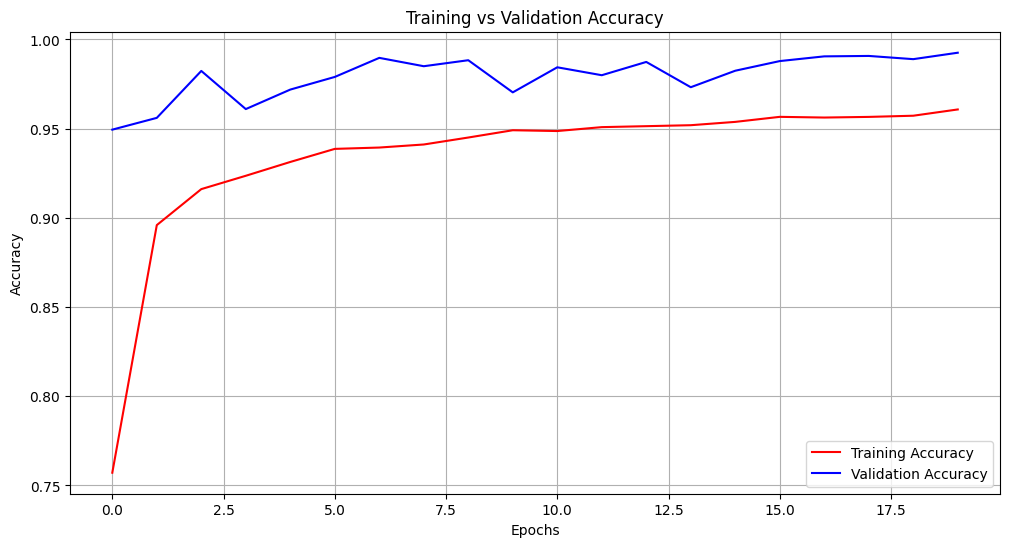
\includegraphics[width=0.45\textwidth]{Assets/validation_accuracy/vgg19.png}
\captionof{figure}{VGG19}

\vspace{0.5cm}

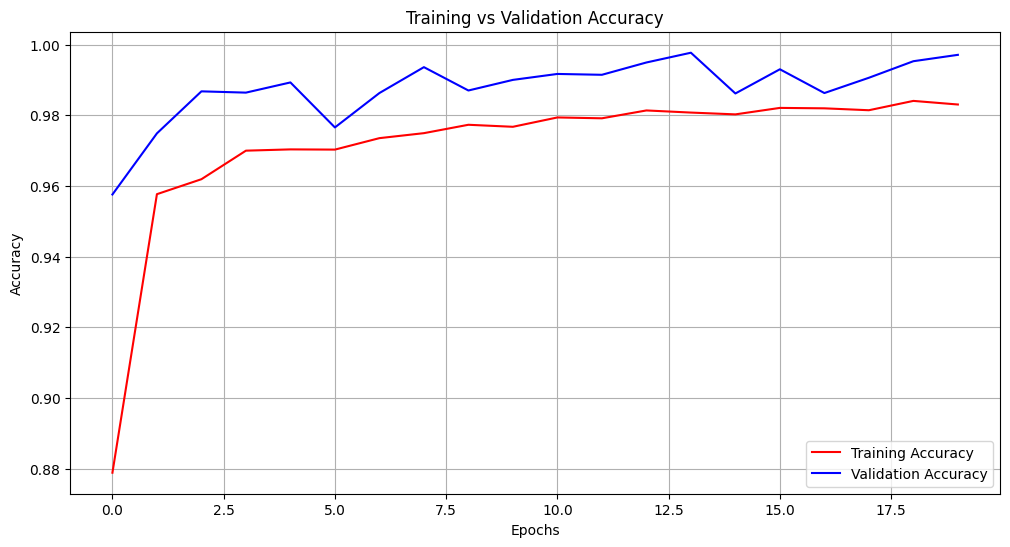
\includegraphics[width=0.45\textwidth]{Assets/validation_accuracy/CONVNEXTBASE.png}
\captionof{figure}{CONVNEXTBASE}

\vspace{0.5cm}

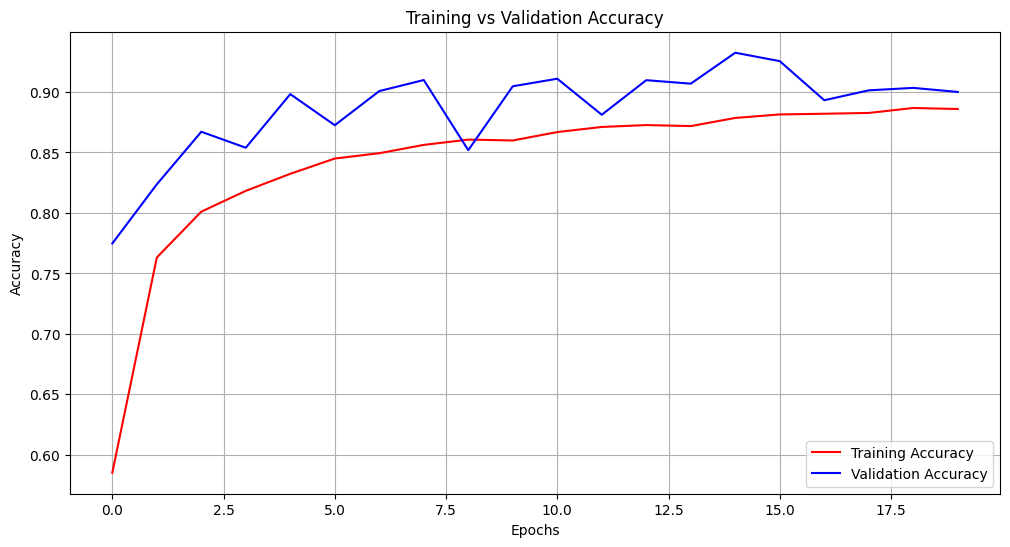
\includegraphics[width=0.45\textwidth]{Assets/validation_accuracy/DENSENET121.png}
\captionof{figure}{DENSENET121}

\vspace{0.5cm}

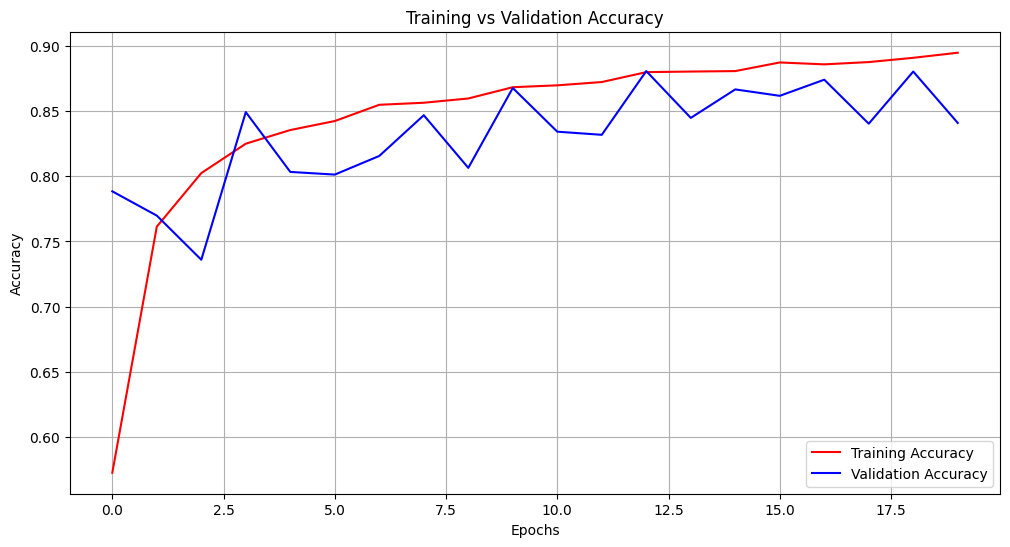
\includegraphics[width=0.45\textwidth]{Assets/validation_accuracy/DenseNet169.png}
\captionof{figure}{DenseNet169}

\vspace{0.5cm}

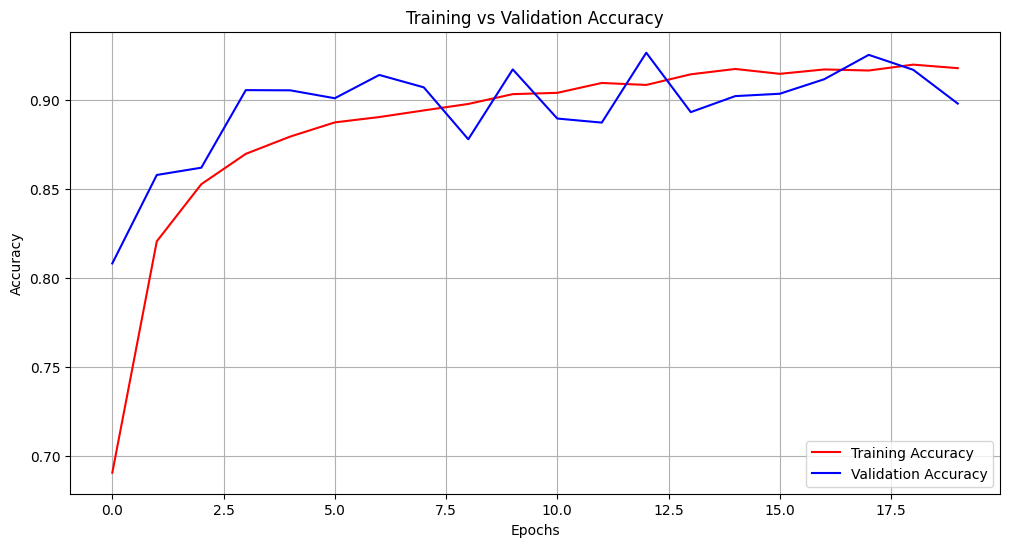
\includegraphics[width=0.45\textwidth]{Assets/validation_accuracy/DENSENET201.png}
\captionof{figure}{DENSENET201}

\vspace{0.5cm}

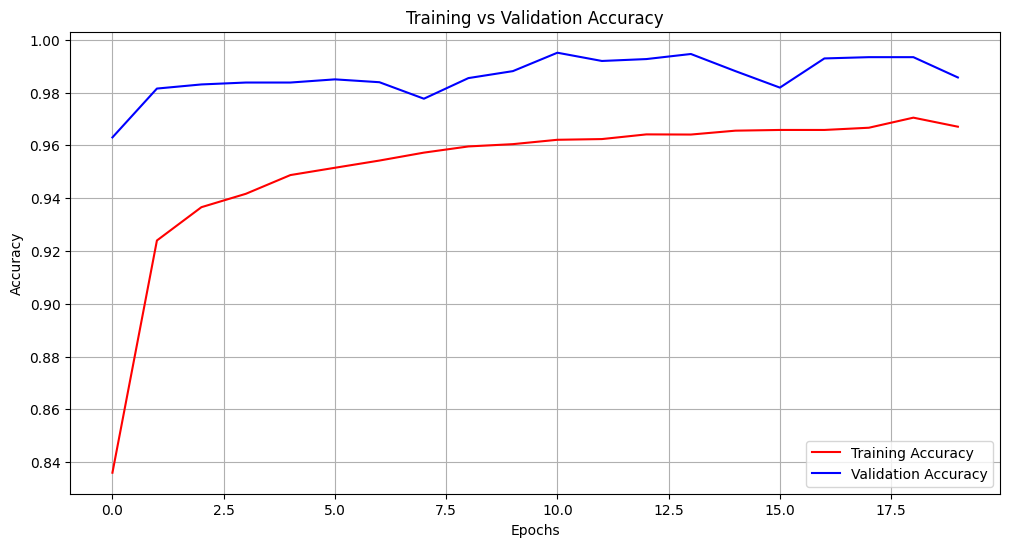
\includegraphics[width=0.45\textwidth]{Assets/validation_accuracy/EfficientNetB0.png}
\captionof{figure}{EfficientNetB0}

\vspace{0.5cm}




\newpage

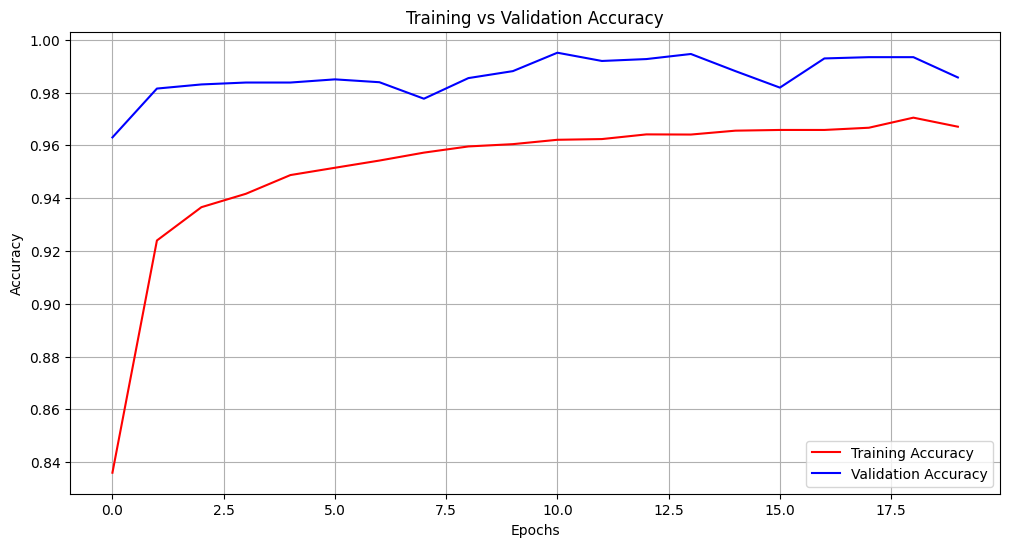
\includegraphics[width=0.45\textwidth]{Assets/validation_accuracy/EfficientNetB0.png}
\captionof{figure}{EfficientNetB1}

\vspace{0.8cm}

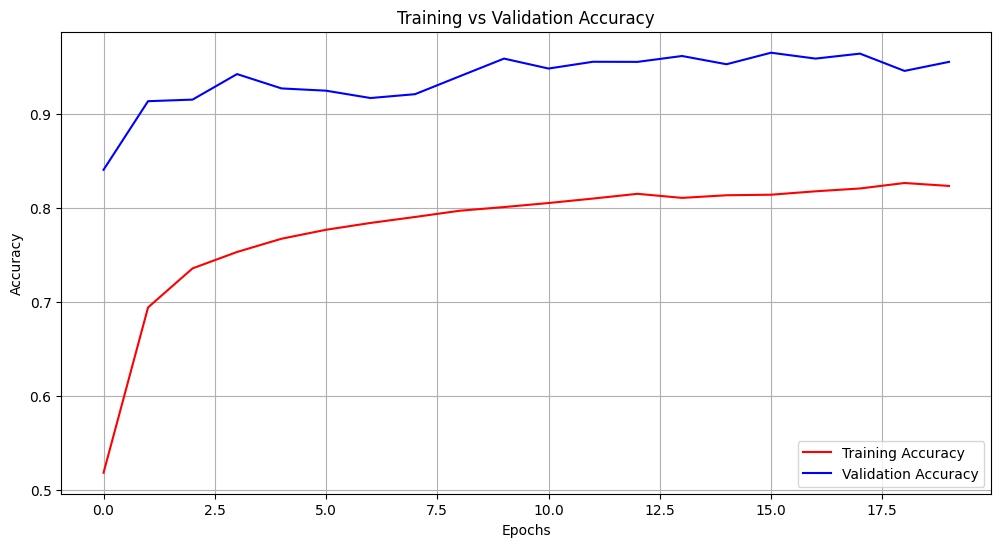
\includegraphics[width=0.45\textwidth]{Assets/validation_accuracy/EfficientNetV2L.png}
\captionof{figure}{EfficientNetV2L}

\vspace{0.8cm}

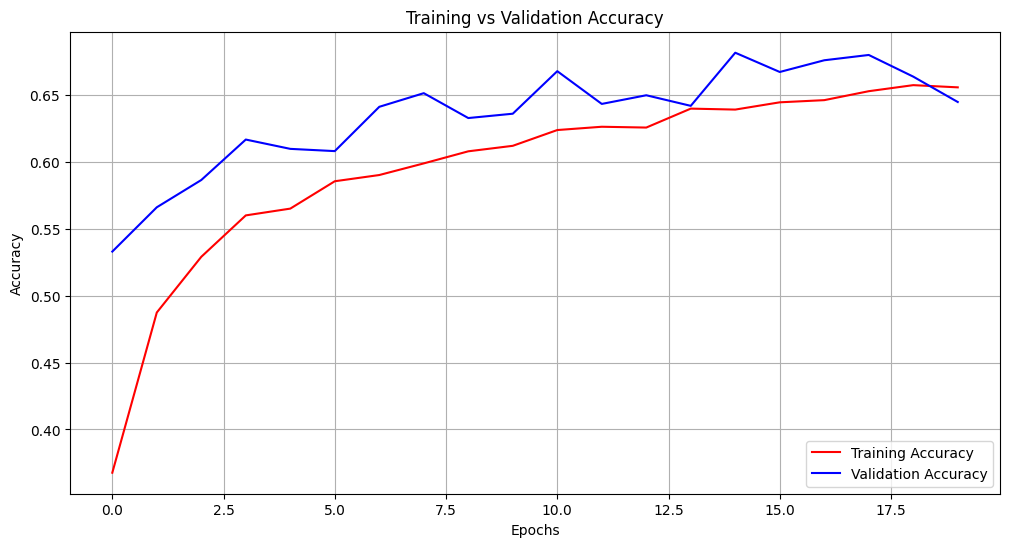
\includegraphics[width=0.45\textwidth]{Assets/validation_accuracy/MOBILENETV2.png}
\captionof{figure}{MOBILENETV2}

\vspace{0.8cm}

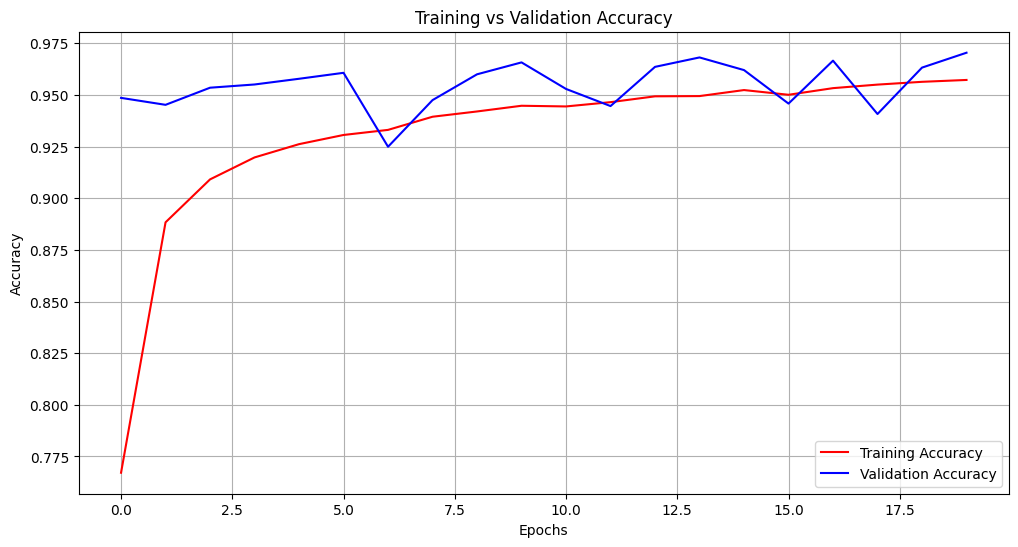
\includegraphics[width=0.45\textwidth]{Assets/validation_accuracy/MobileNetV3Large.png}
\captionof{figure}{MobileNetV3Large}

\vspace{0.8cm}

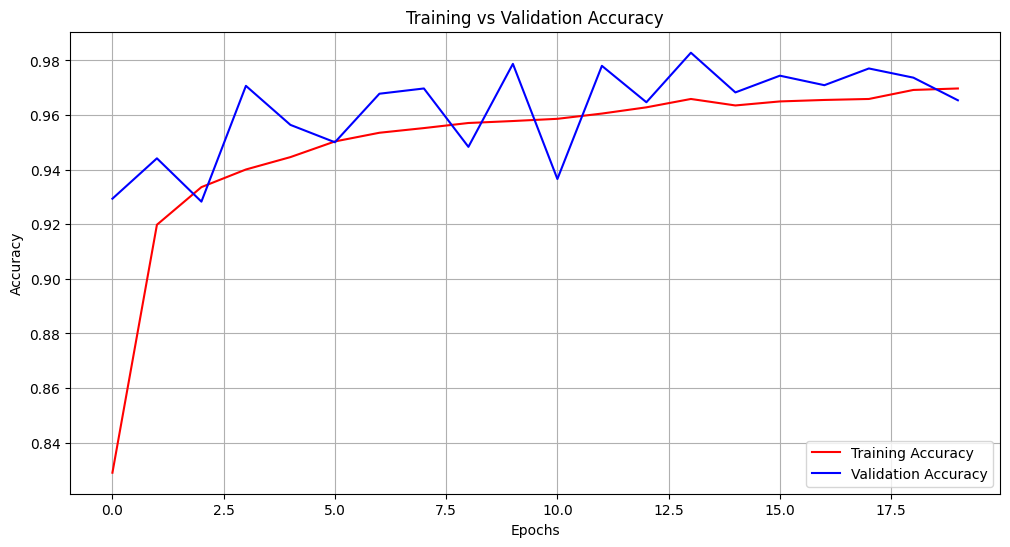
\includegraphics[width=0.45\textwidth]{Assets/validation_accuracy/ResNet50.png}
\captionof{figure}{ResNet50}

\vspace{0.8cm}

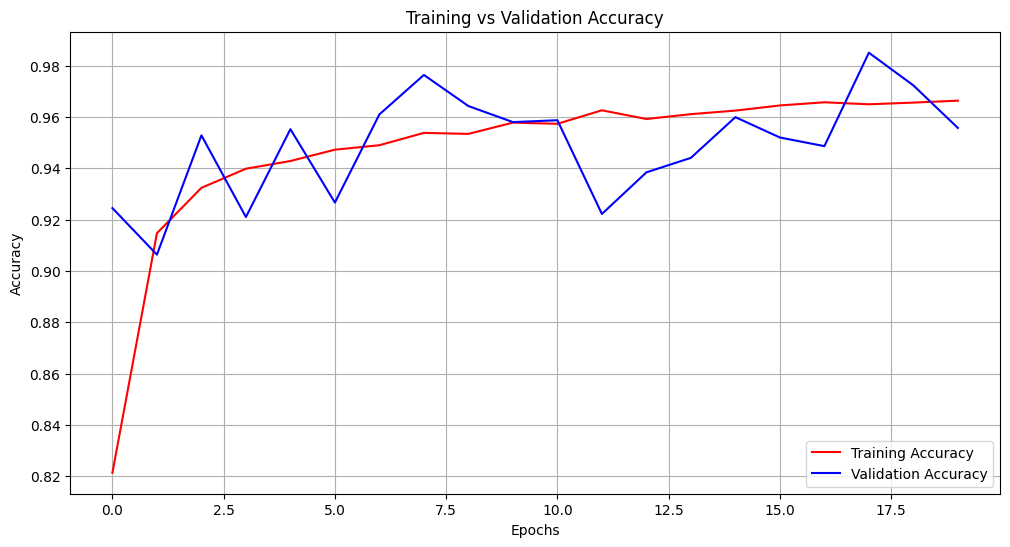
\includegraphics[width=0.45\textwidth]{Assets/validation_accuracy/RESNET101.png}
\captionof{figure}{RESNET101}

\vspace{0.8cm}

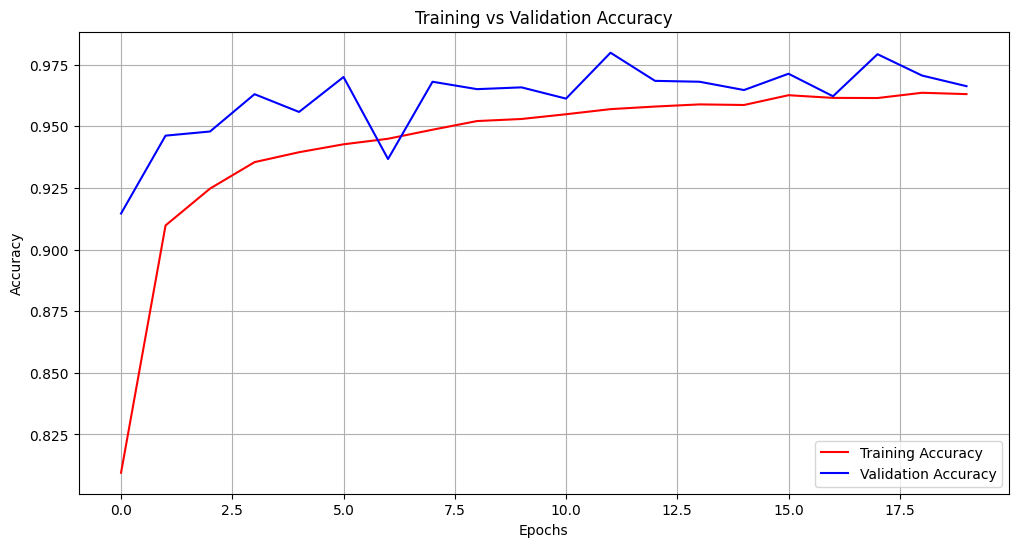
\includegraphics[width=0.45\textwidth]{Assets/validation_accuracy/RESNET152.png}
\captionof{figure}{RESNET152}

\vspace{0.8cm}

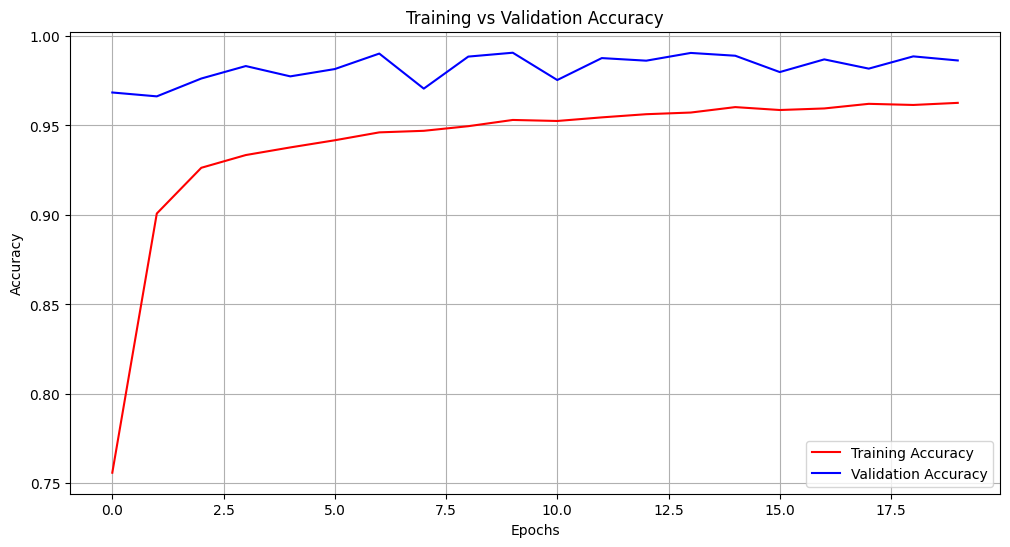
\includegraphics[width=0.45\textwidth]{Assets/validation_accuracy/vgg16.png}
\captionof{figure}{VGG16}

\vspace{0.8cm}

\end{multicols}

\newpage

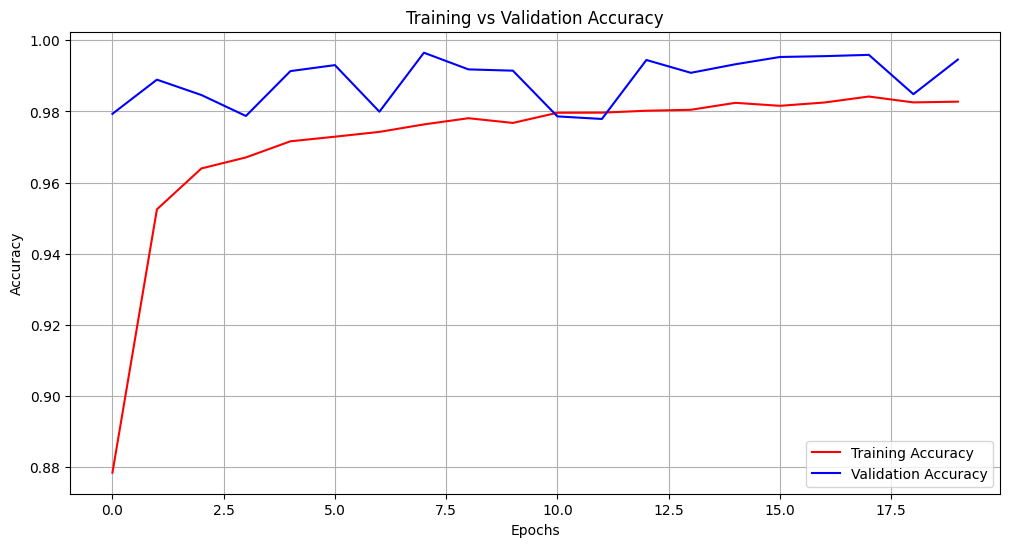
\includegraphics[width=0.9\textwidth]{Assets/validation_accuracy/CONVNEXT.png}
\captionof{figure}{CONVNEXT}





% \chapter*{Appendix-II: Training vs. Validation Loss Graphs}
\addcontentsline{toc}{chapter}{Appendix-II: Training vs Validation Loss Graphs}

\noindent This appendix contains the training vs. validation loss graphs for all models.

\begin{multicols}{2}
\centering

\setcounter{figure}{0} % Reset figure counter
\renewcommand{\thefigure}{2.\arabic{figure}} % Prefix figures with "2."

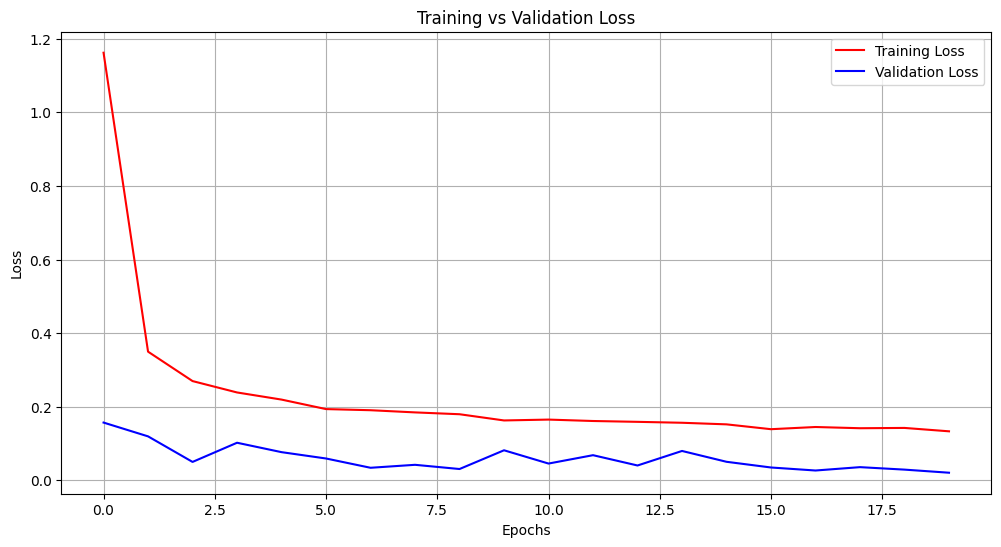
\includegraphics[width=0.45\textwidth]{Assets/validation_loss/vgg19.png}
\captionof{figure}{VGG19}

\vspace{0.5cm}

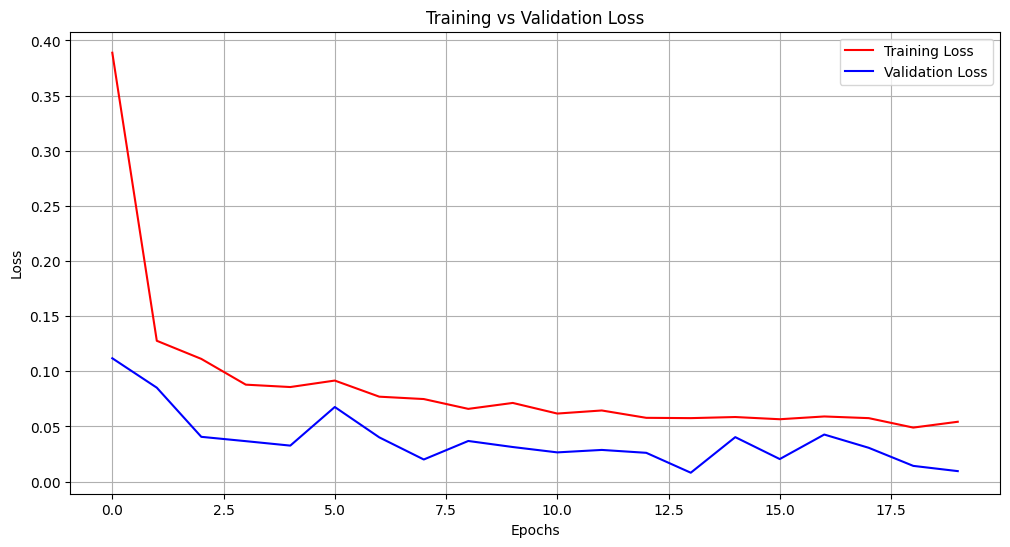
\includegraphics[width=0.45\textwidth]{Assets/validation_loss/CONVNEXTBASE.png}
\captionof{figure}{CONVNEXTBASE}

\vspace{0.5cm}

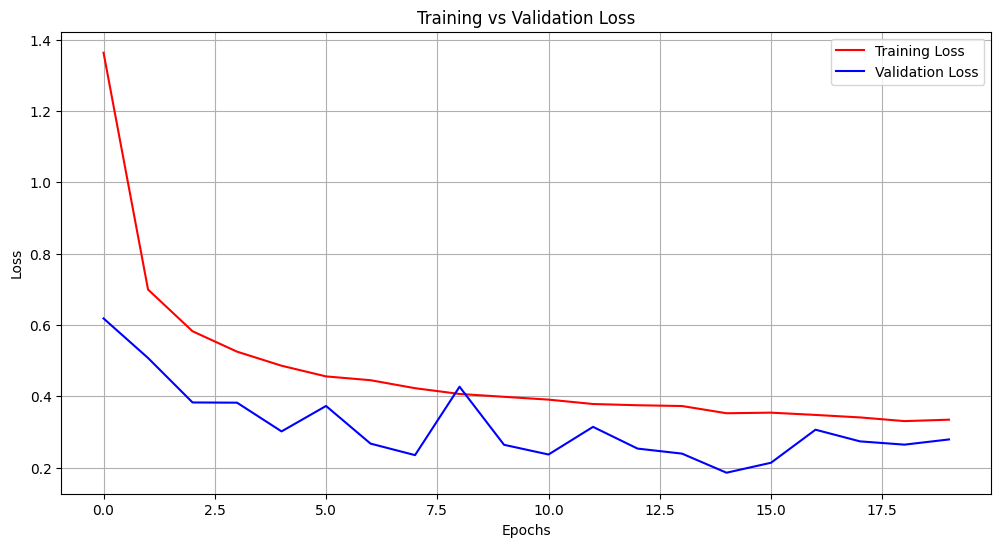
\includegraphics[width=0.45\textwidth]{Assets/validation_loss/DENSENET121.png}
\captionof{figure}{DENSENET121}

\vspace{0.5cm}

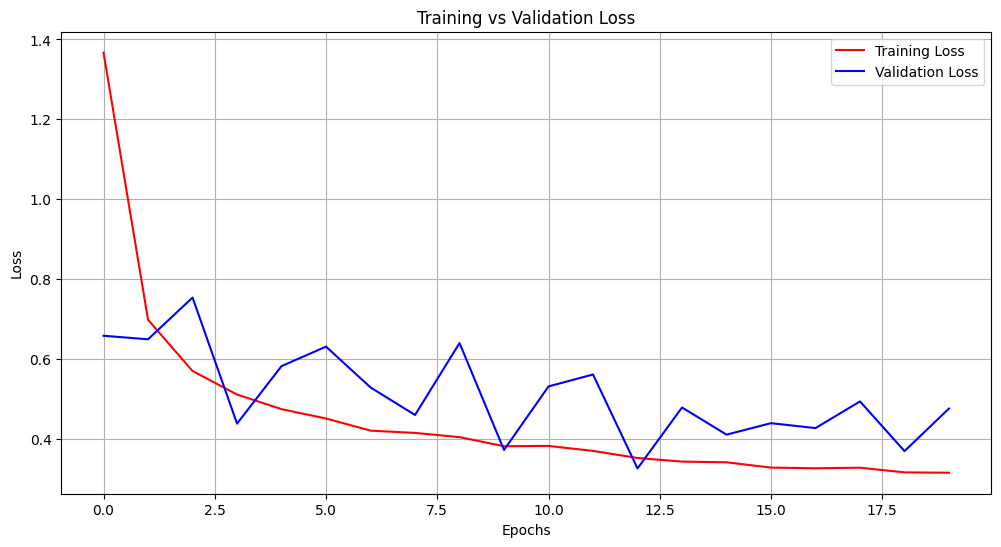
\includegraphics[width=0.45\textwidth]{Assets/validation_loss/DenseNet169.png}
\captionof{figure}{DenseNet169}

\vspace{0.5cm}

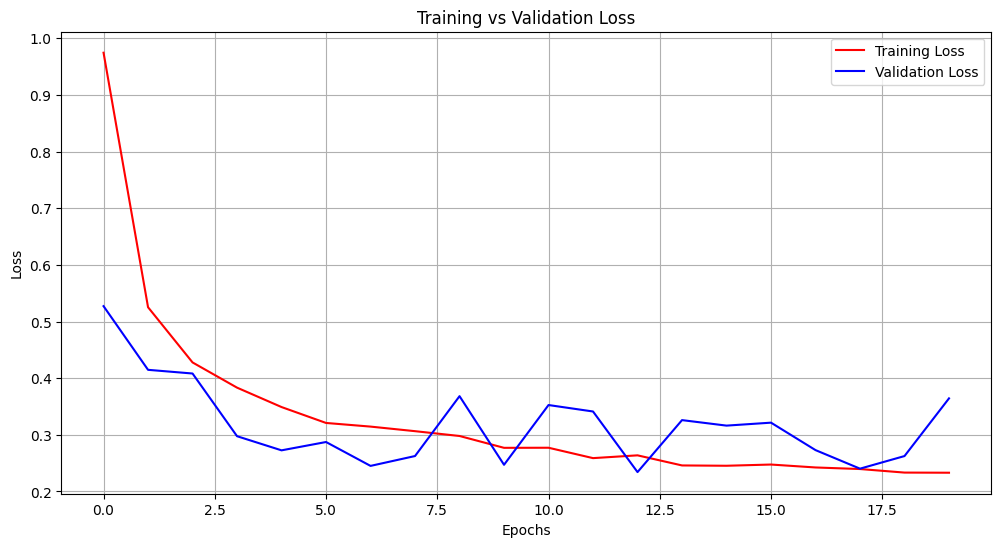
\includegraphics[width=0.45\textwidth]{Assets/validation_loss/DENSENET201.png}
\captionof{figure}{DENSENET201}

\vspace{0.5cm}

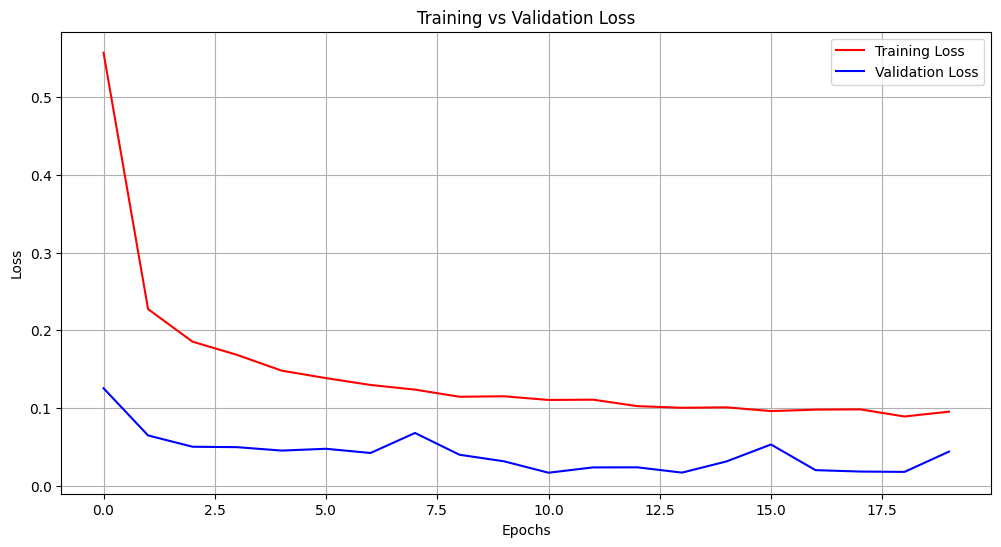
\includegraphics[width=0.45\textwidth]{Assets/validation_loss/EfficientNetB0.png}
\captionof{figure}{EfficientNetB0}

\vspace{0.5cm}

\newpage

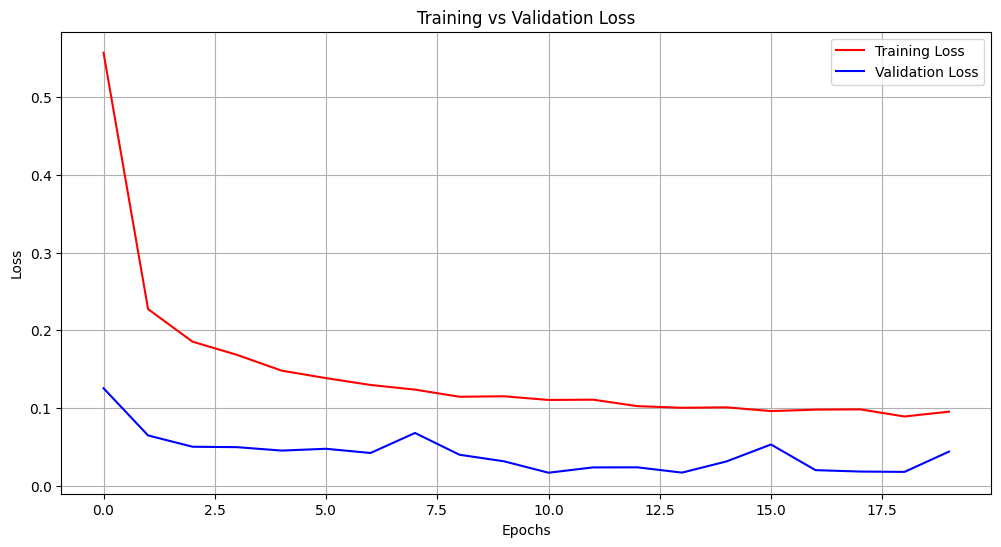
\includegraphics[width=0.45\textwidth]{Assets/validation_loss/EfficientNetB0.png}
\captionof{figure}{EfficientNetB1}

\vspace{0.8cm}

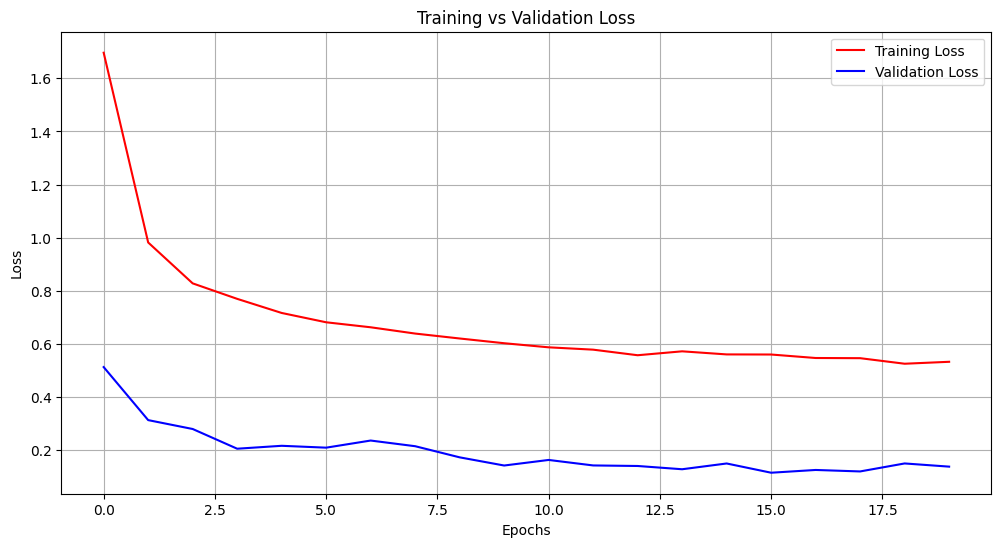
\includegraphics[width=0.45\textwidth]{Assets/validation_loss/EfficientNetV2L.png}
\captionof{figure}{EfficientNetV2L}

\vspace{0.8cm}

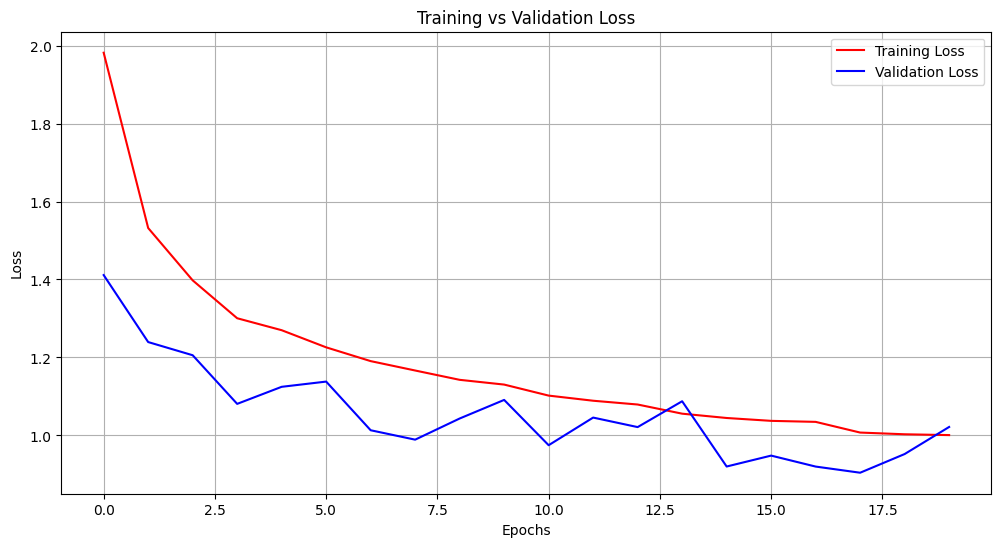
\includegraphics[width=0.45\textwidth]{Assets/validation_loss/MOBILENETV2.png}
\captionof{figure}{MOBILENETV2}

\vspace{0.8cm}

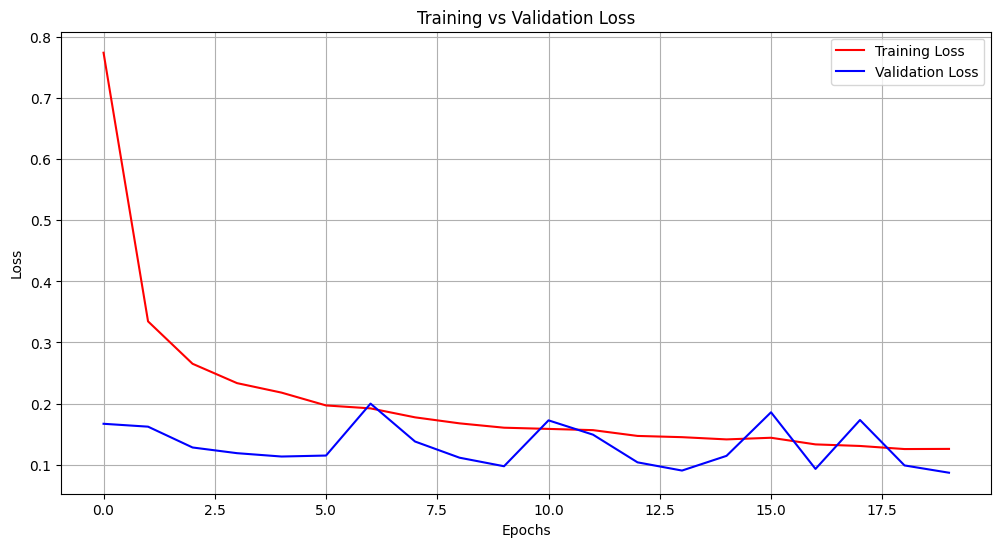
\includegraphics[width=0.45\textwidth]{Assets/validation_loss/MobileNetV3Large.png}
\captionof{figure}{MobileNetV3Large}

\vspace{0.8cm}

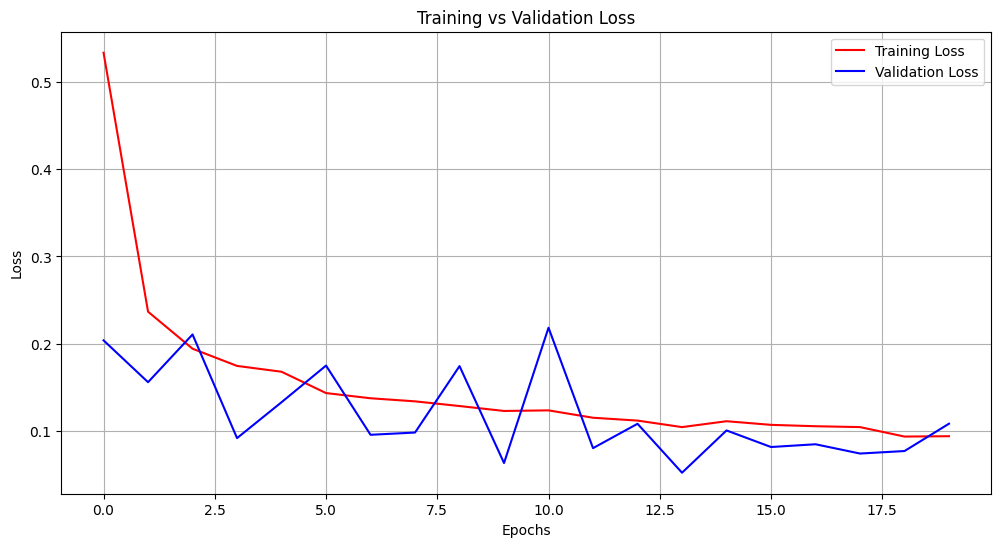
\includegraphics[width=0.45\textwidth]{Assets/validation_loss/ResNet50.png}
\captionof{figure}{ResNet50}

\vspace{0.8cm}

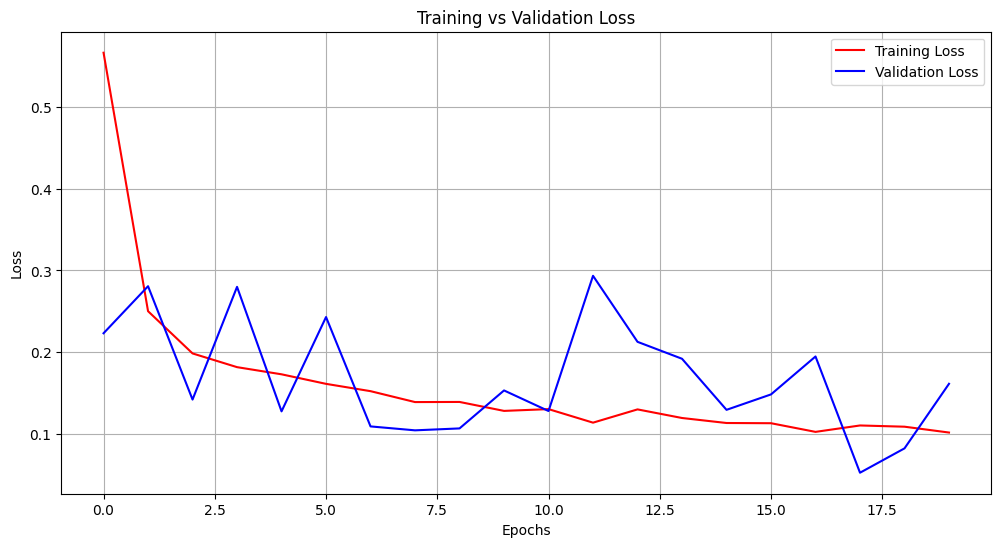
\includegraphics[width=0.45\textwidth]{Assets/validation_loss/RESNET101.png}
\captionof{figure}{RESNET101}

\vspace{0.8cm}

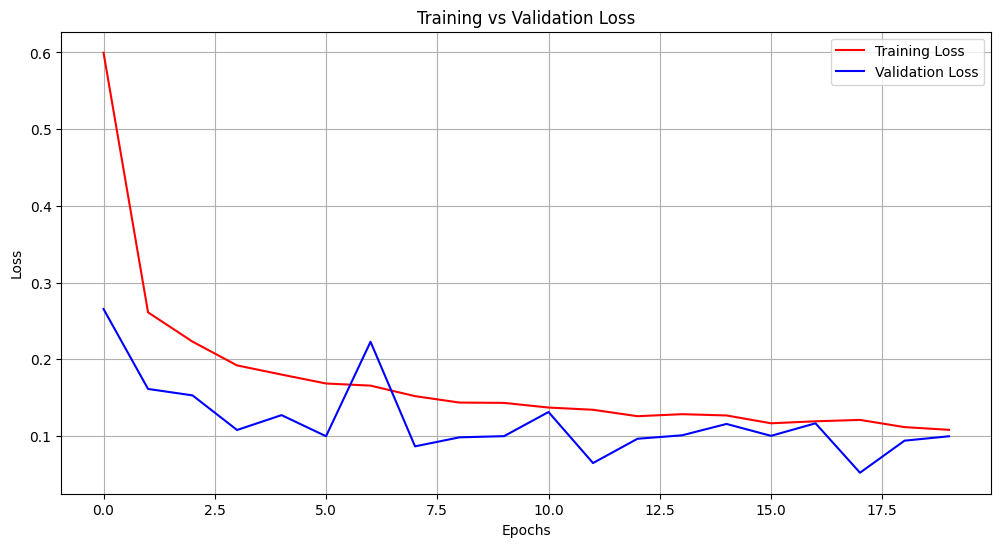
\includegraphics[width=0.45\textwidth]{Assets/validation_loss/RESNET152.png}
\captionof{figure}{RESNET152}

\vspace{0.8cm}

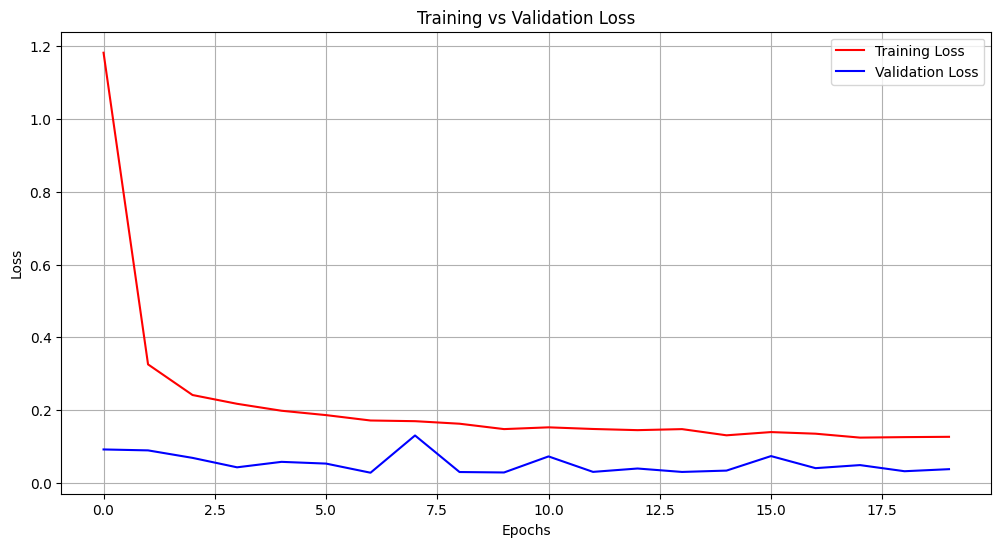
\includegraphics[width=0.45\textwidth]{Assets/validation_loss/vgg16.png}
\captionof{figure}{VGG16}

\vspace{0.8cm}

\end{multicols}

\newpage

\renewcommand{\thefigure}{2.\arabic{figure}} % Prefix figures with "2."

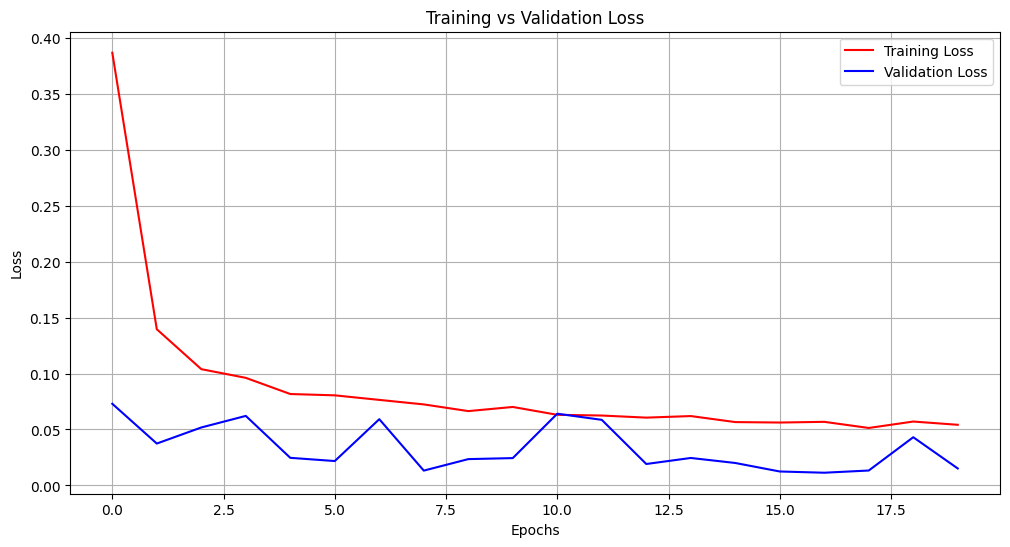
\includegraphics[width=0.9\textwidth]{Assets/validation_loss/CONVNEXT.png}
\captionof{figure}{CONVNEXT}

% \chapter*{Appendix-III: Confusion Matrices}
\addcontentsline{toc}{chapter}{Appendix-III: Confusion Matrices}

\noindent This appendix contains the confusion matrices for all models.

\setcounter{figure}{0} % Reset figure counter
\renewcommand{\thefigure}{2.\arabic{figure}} % Prefix figures with "2."

% First page with only one confusion matrix
\begin{figure}[h!]
    \centering
    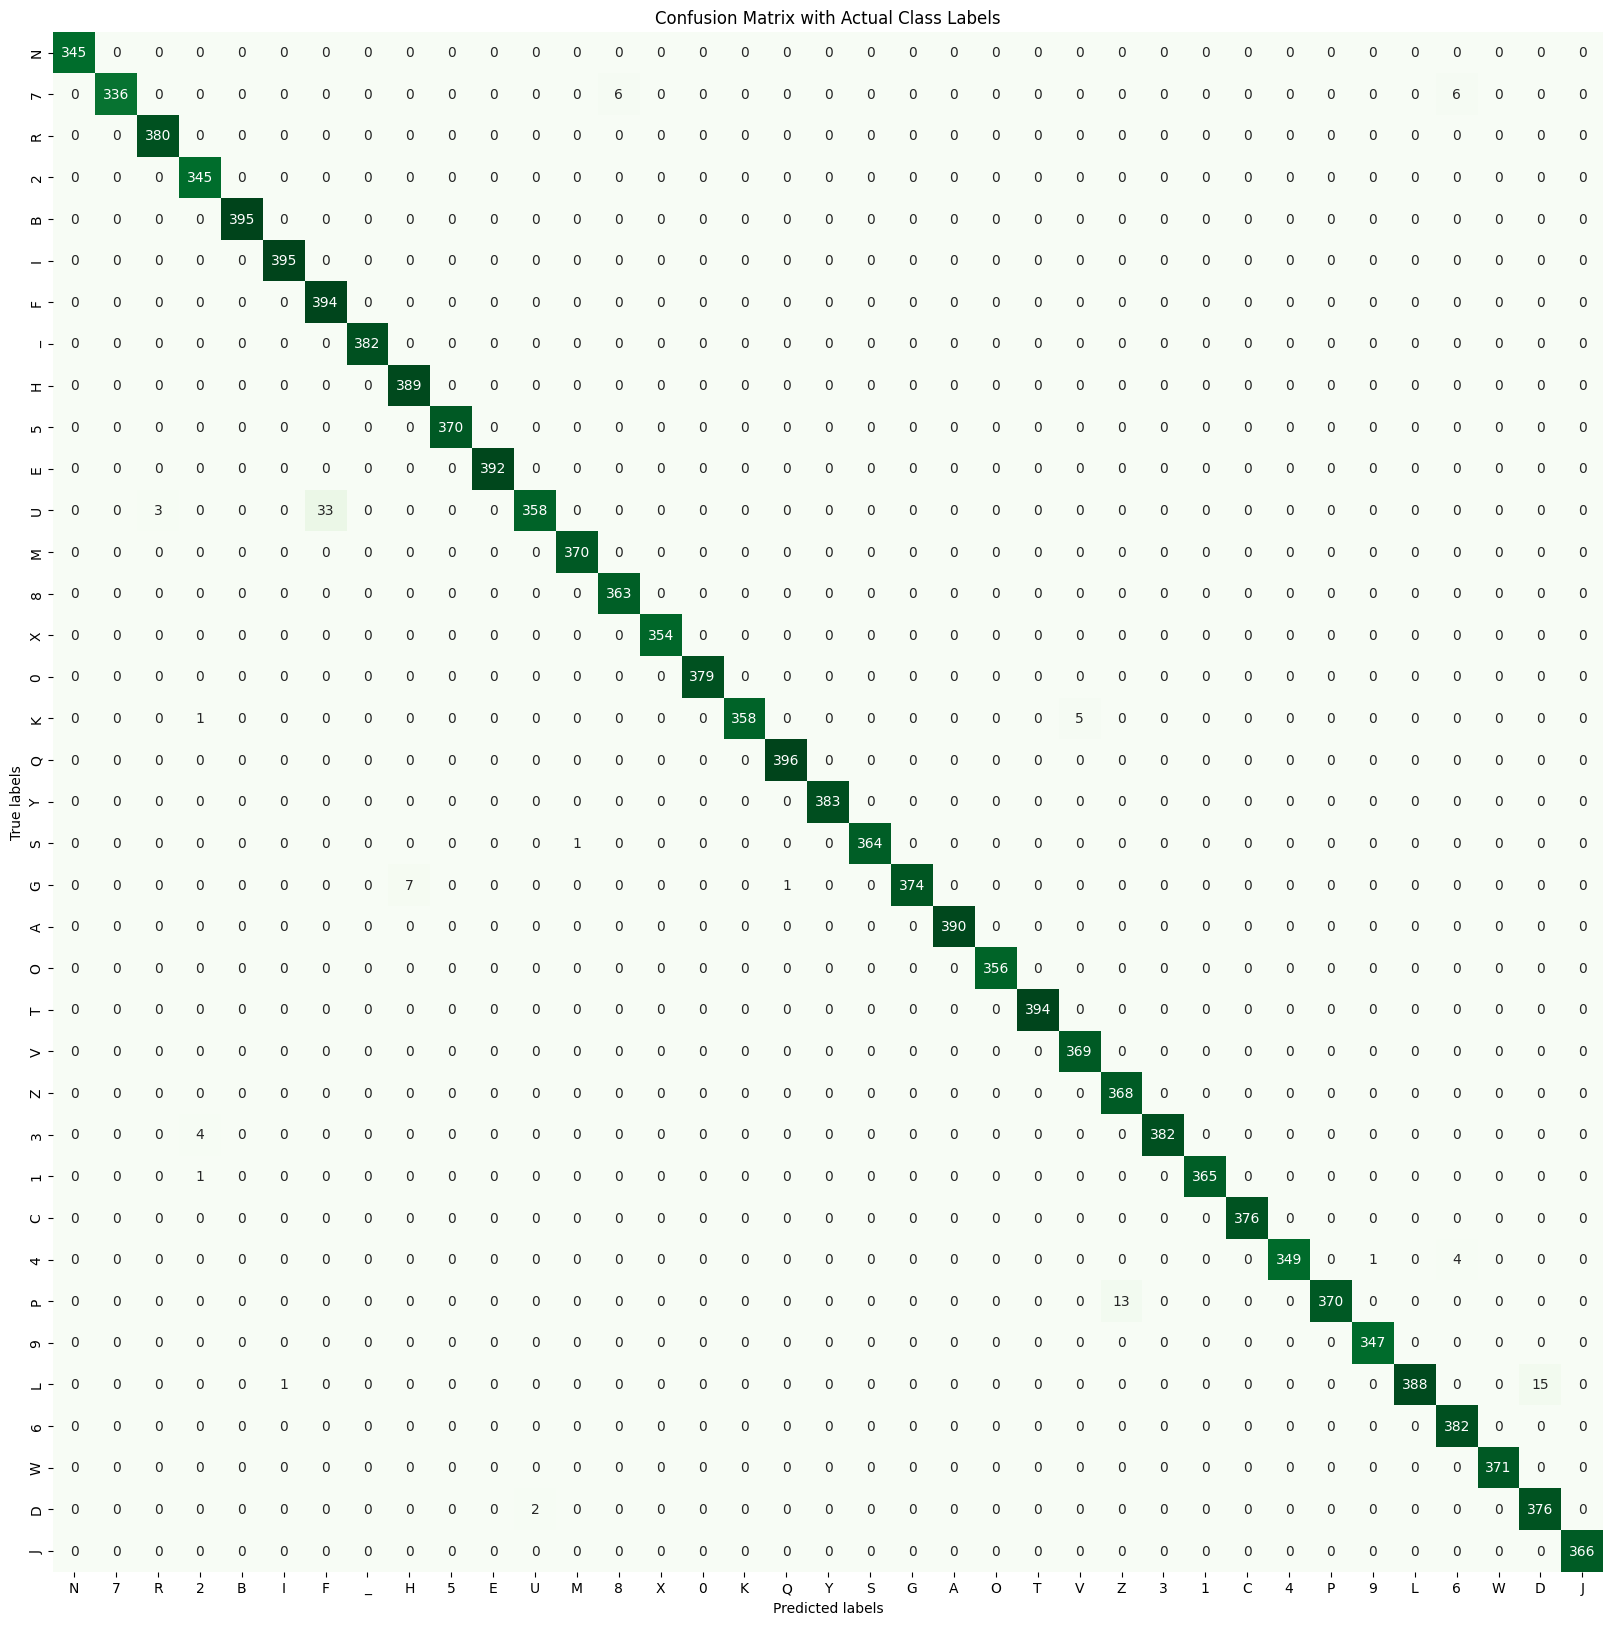
\includegraphics[width=0.9\textwidth]{Assets/confusion_matrix/vgg19.png}
    \caption{Confusion Matrix: VGG19}
\end{figure}

\newpage

% Subsequent pages with two confusion matrices per page
\begin{figure}[h!]
    \centering
    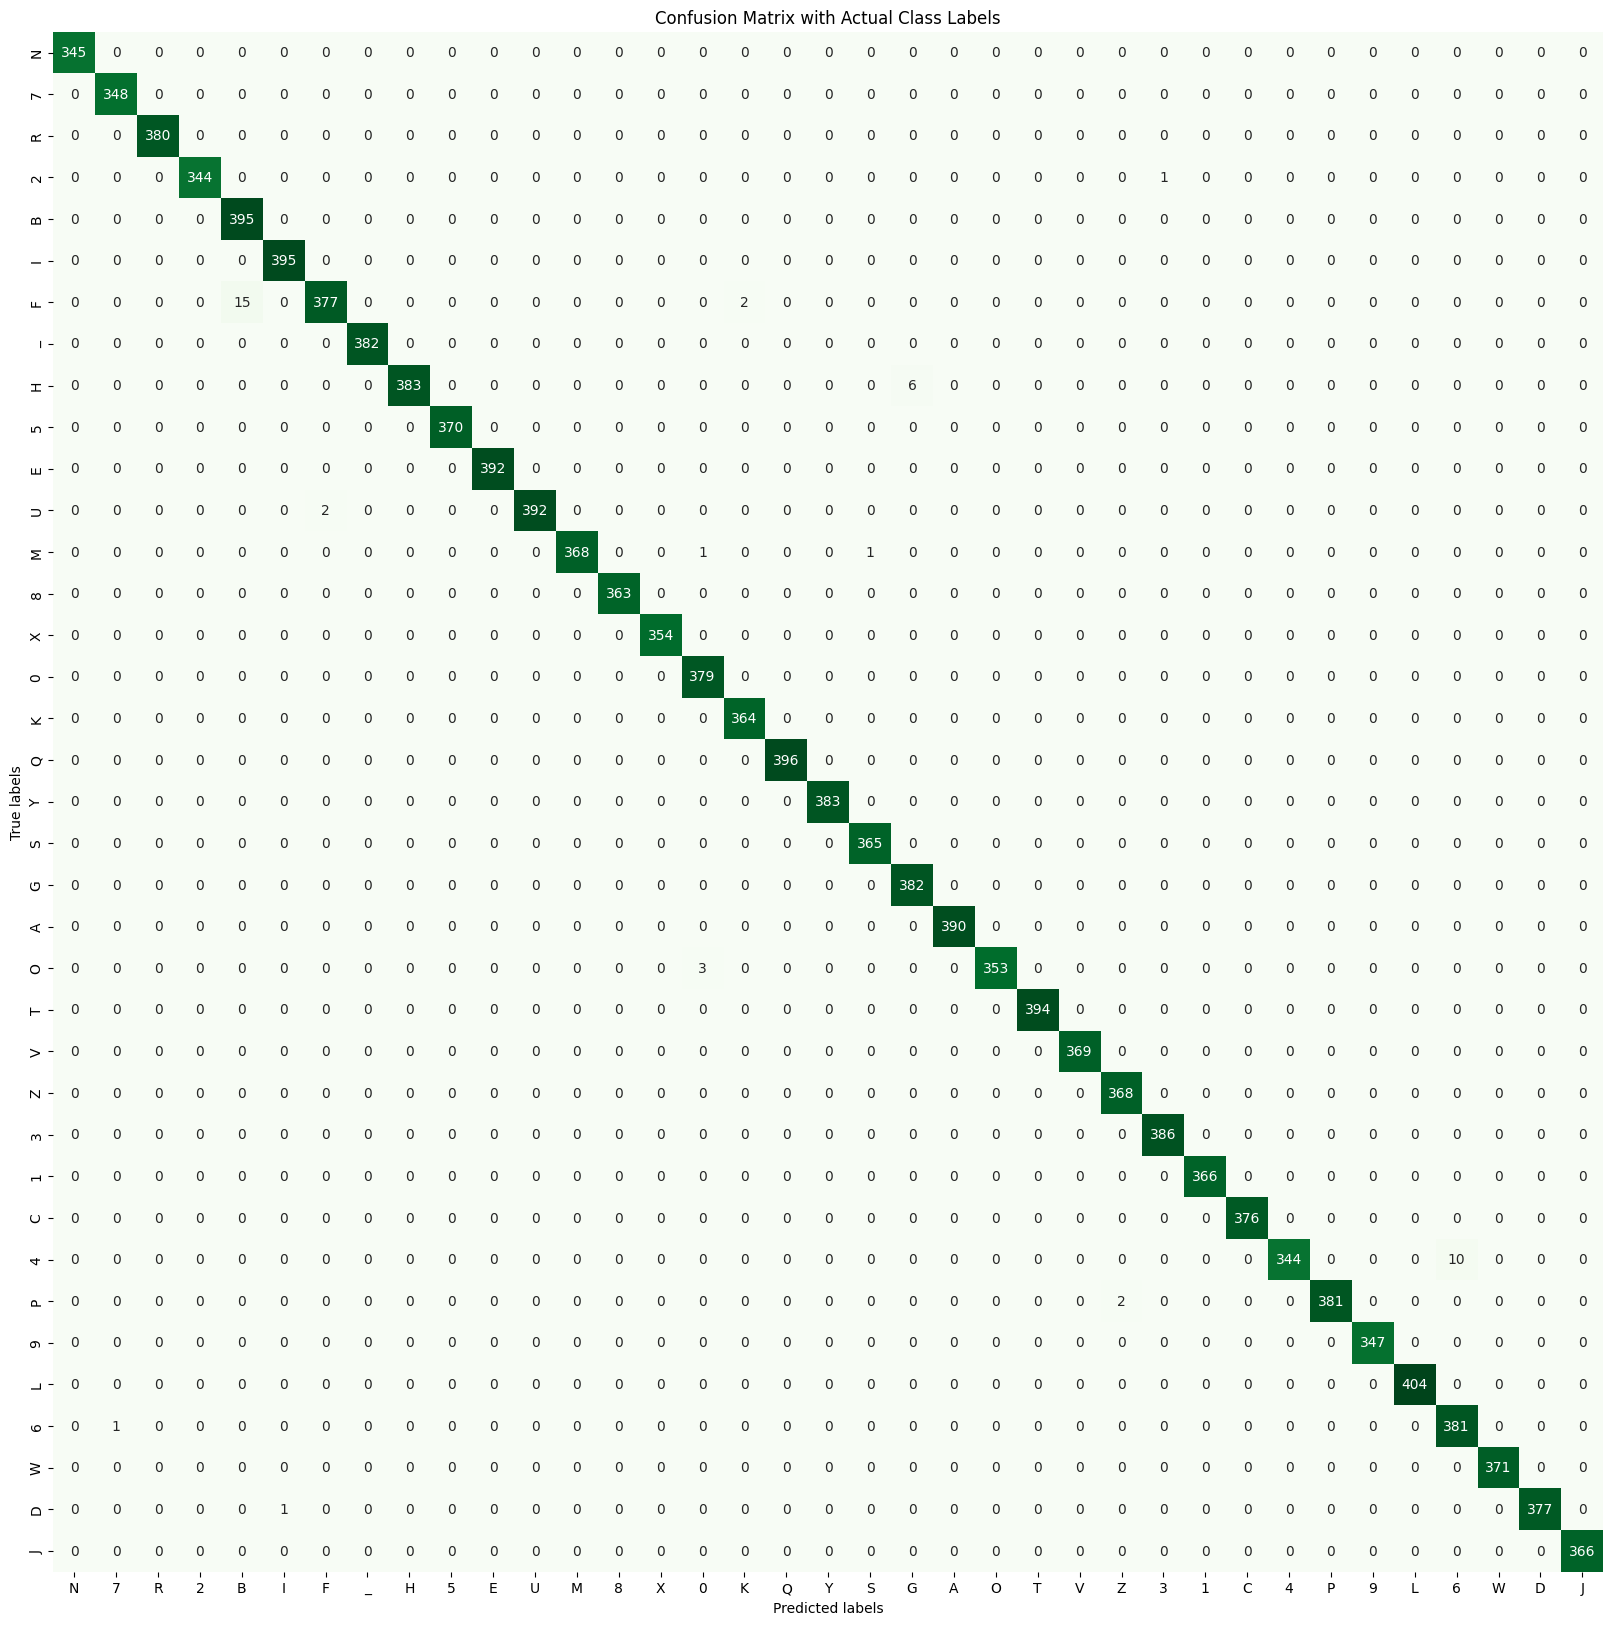
\includegraphics[width=0.55\textwidth]{Assets/confusion_matrix/CONVNEXTBASE.png}
    \caption{Confusion Matrix: CONVNEXTBASE}
    \vspace{1.5cm} % Add some space between the two figures
    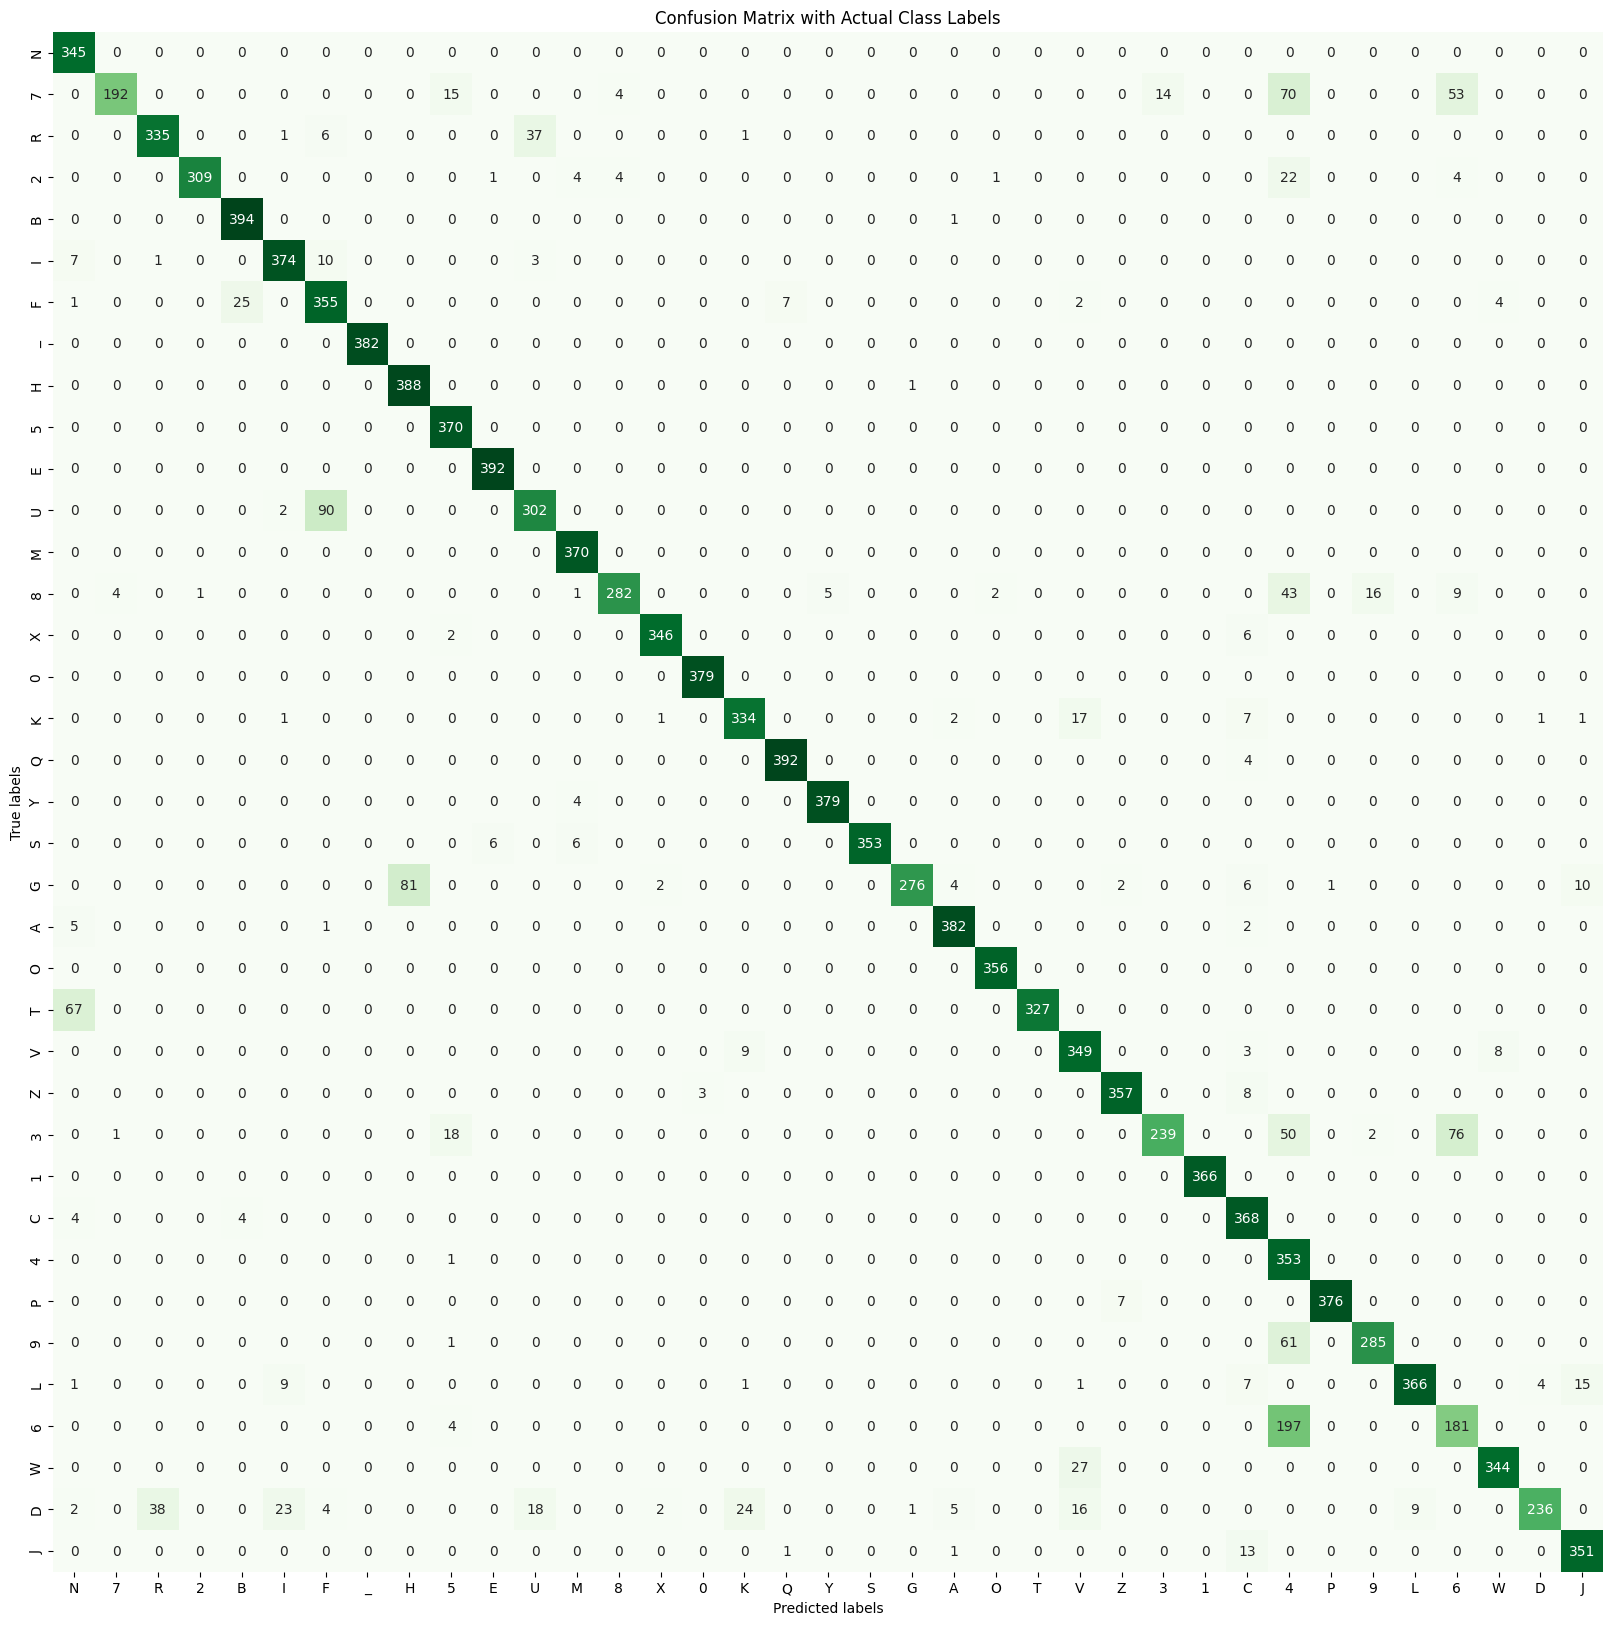
\includegraphics[width=0.55\textwidth]{Assets/confusion_matrix/DENSENET121.png}
    \caption{Confusion Matrix: DENSENET121}
\end{figure}

\newpage

\begin{figure}[h!]
    \centering
    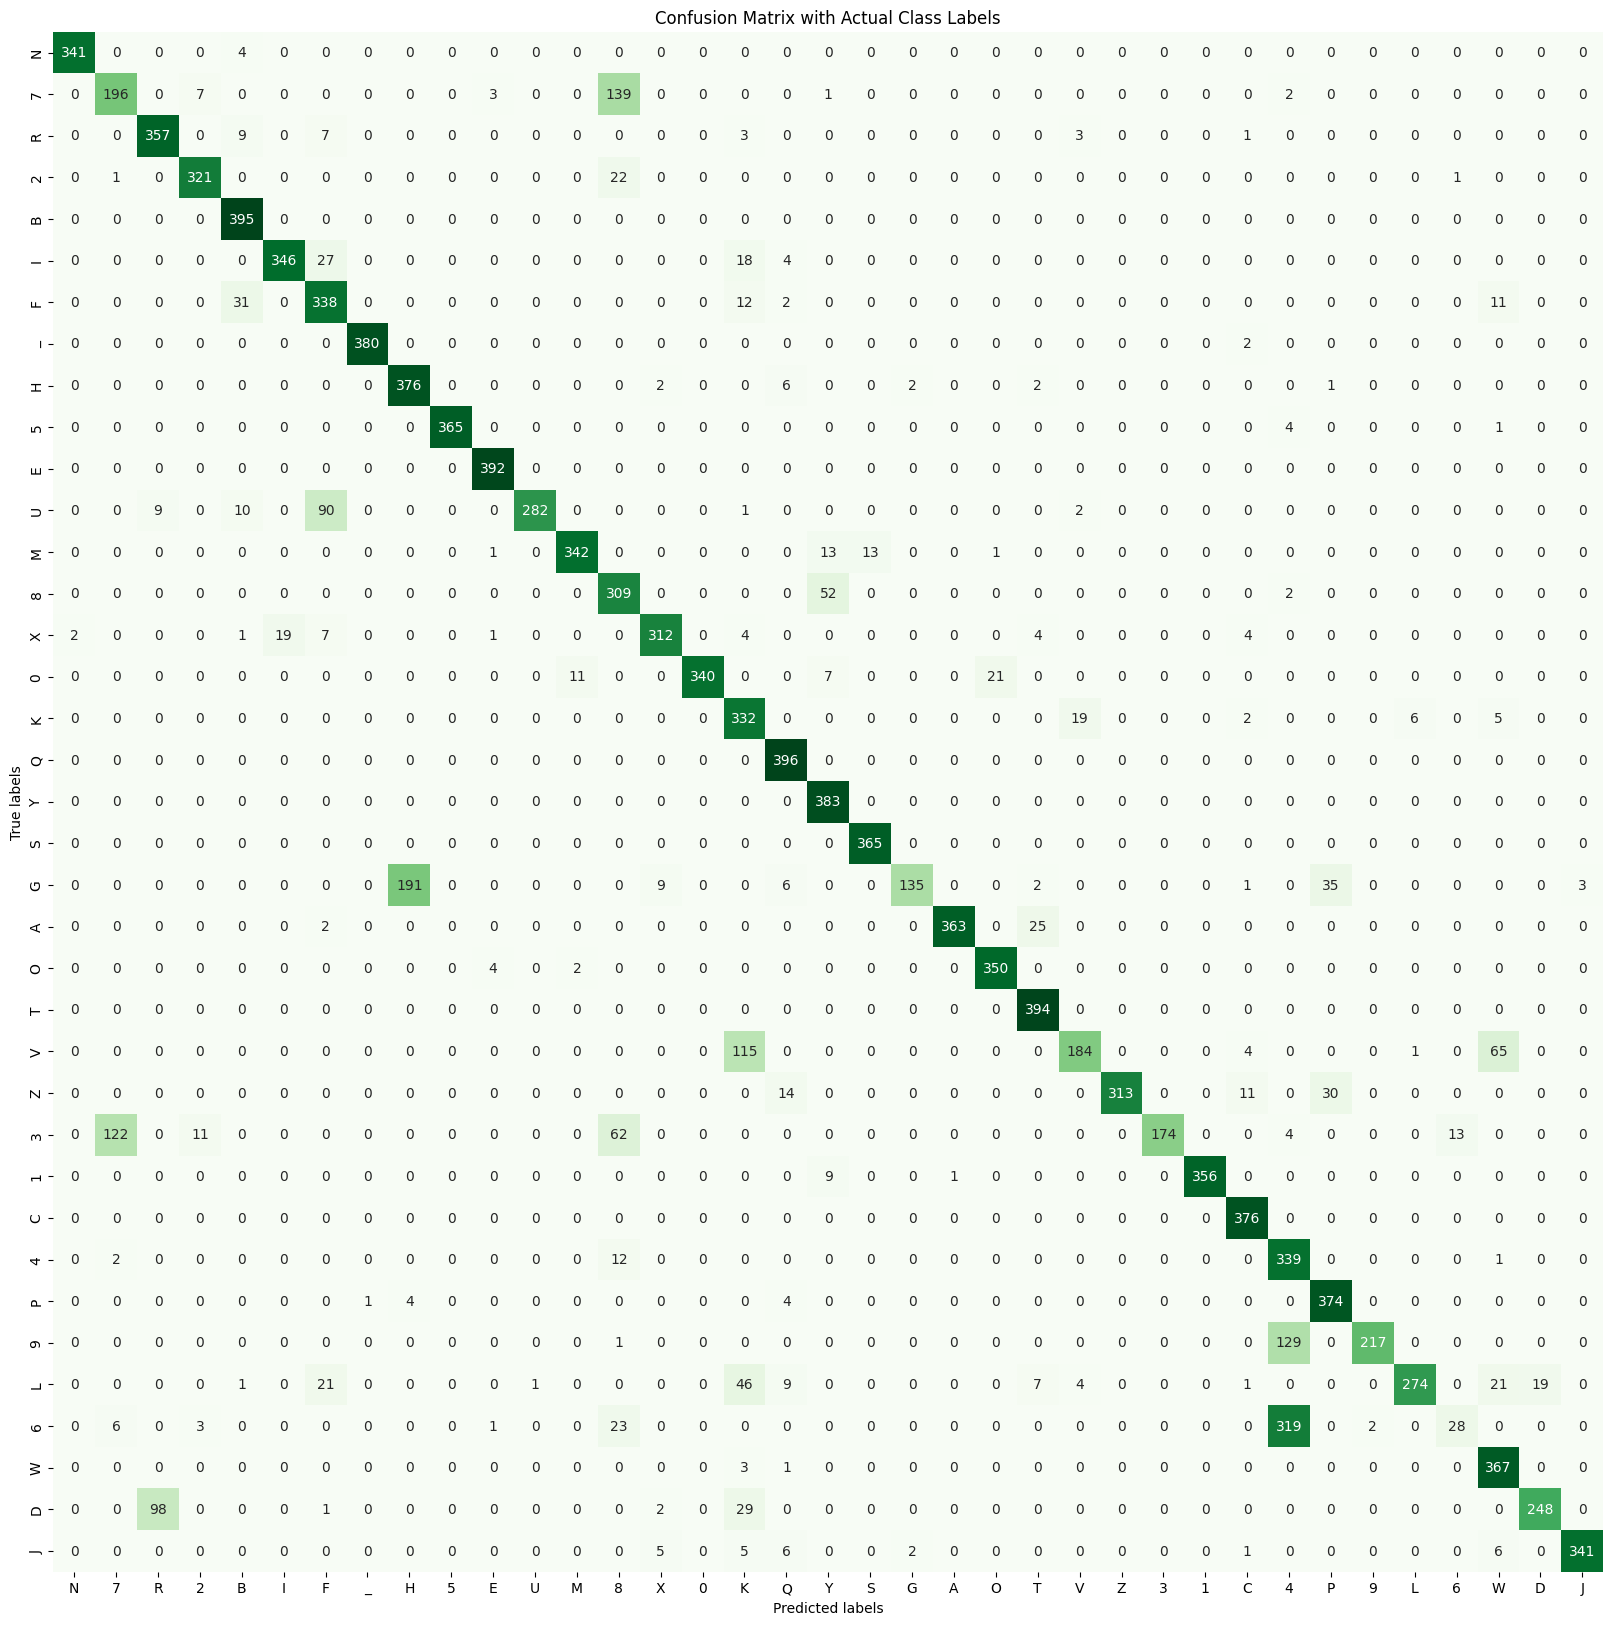
\includegraphics[width=0.55\textwidth]{Assets/confusion_matrix/DenseNet169.png}
    \caption{Confusion Matrix: DenseNet169}
    \vspace{1.5cm}
    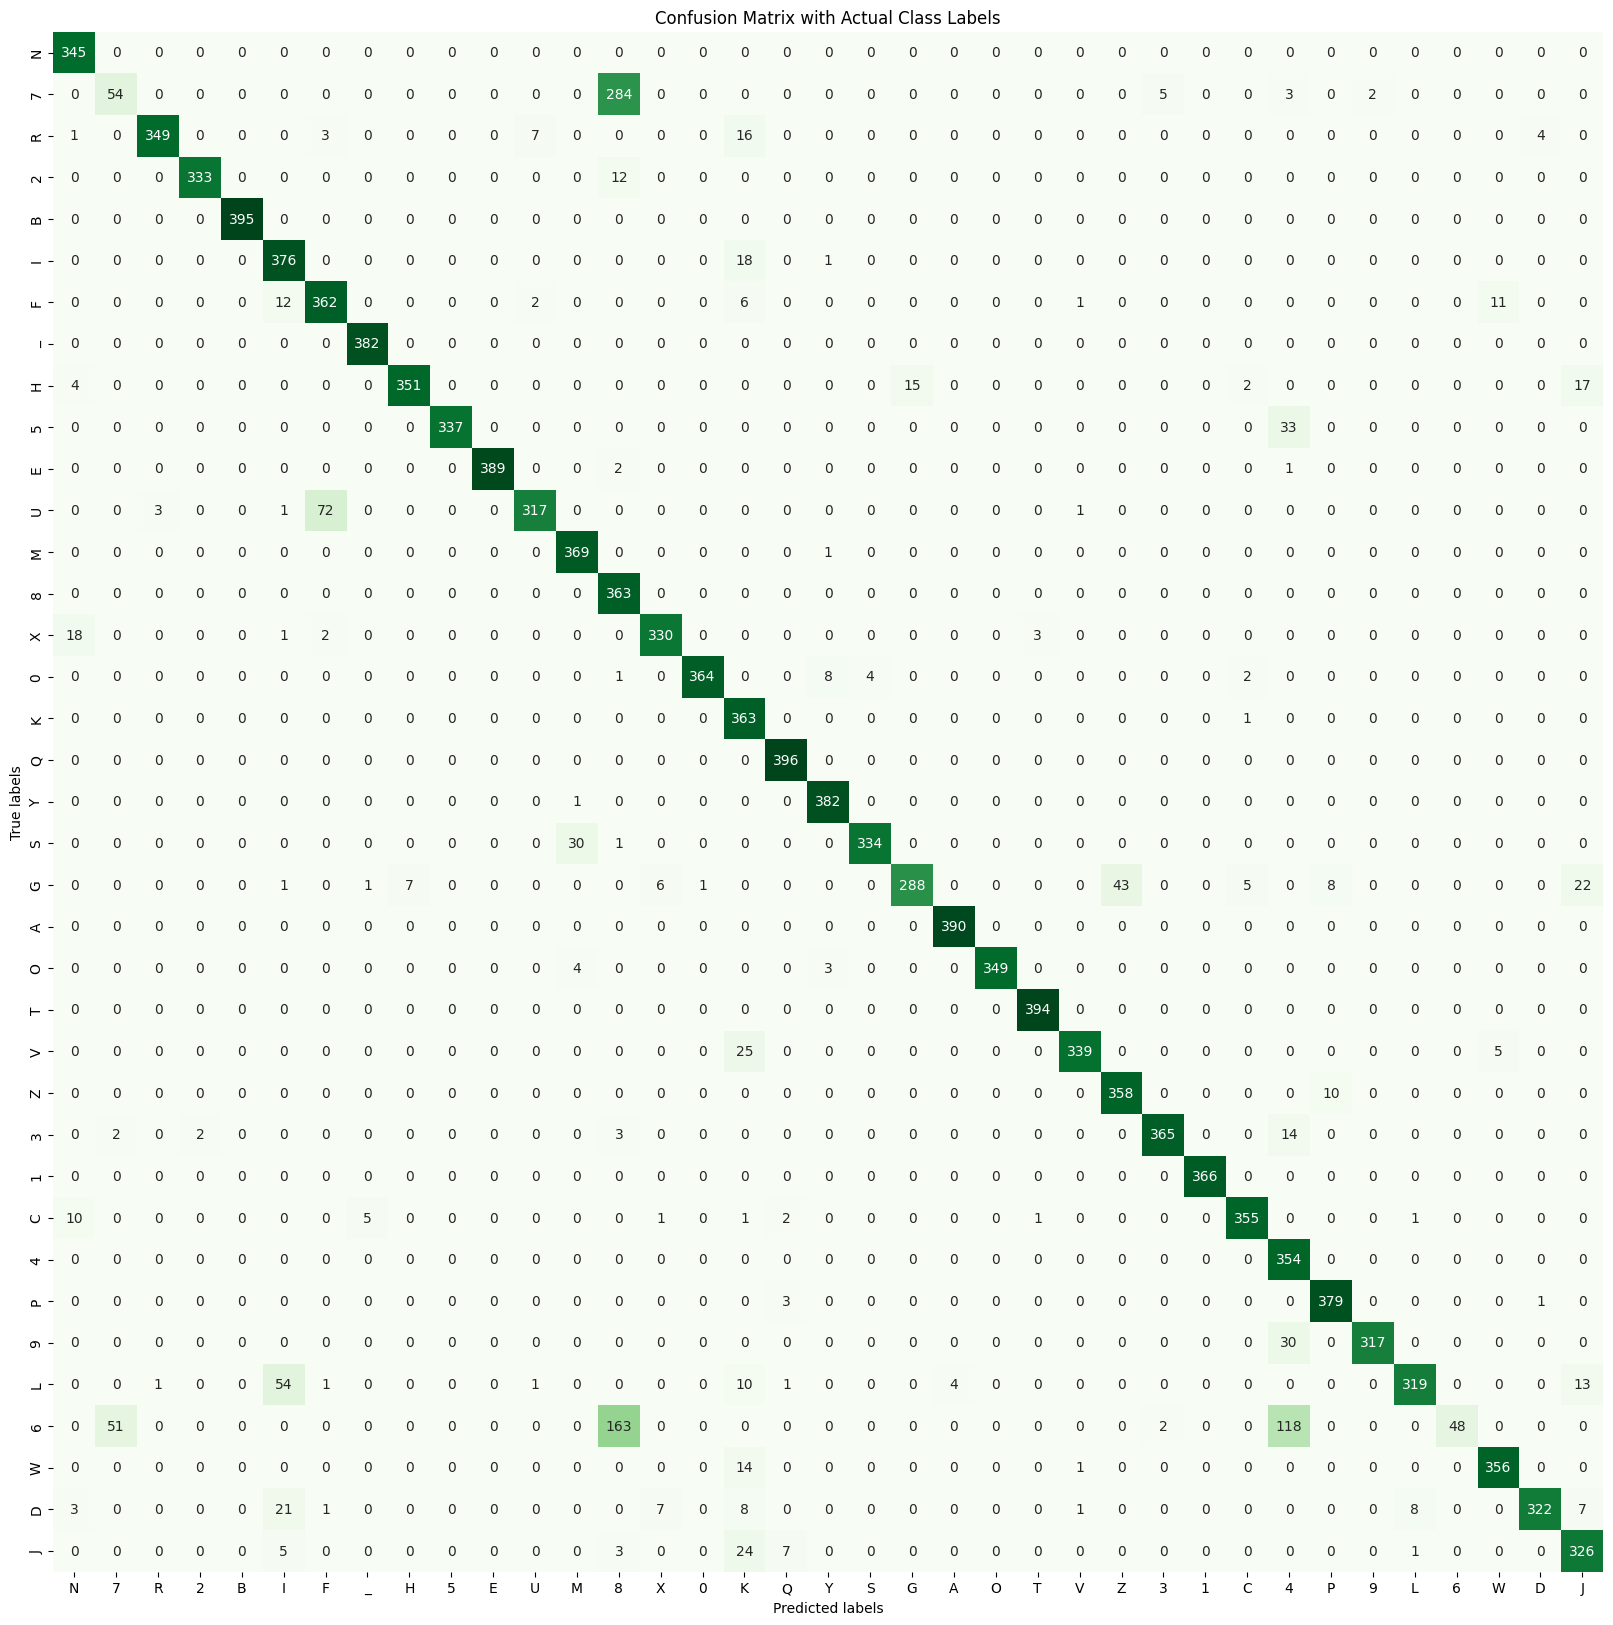
\includegraphics[width=0.55\textwidth]{Assets/confusion_matrix/DENSENET201.png}
    \caption{Confusion Matrix: DENSENET201}
\end{figure}

\newpage

\begin{figure}[h!]
    \centering
    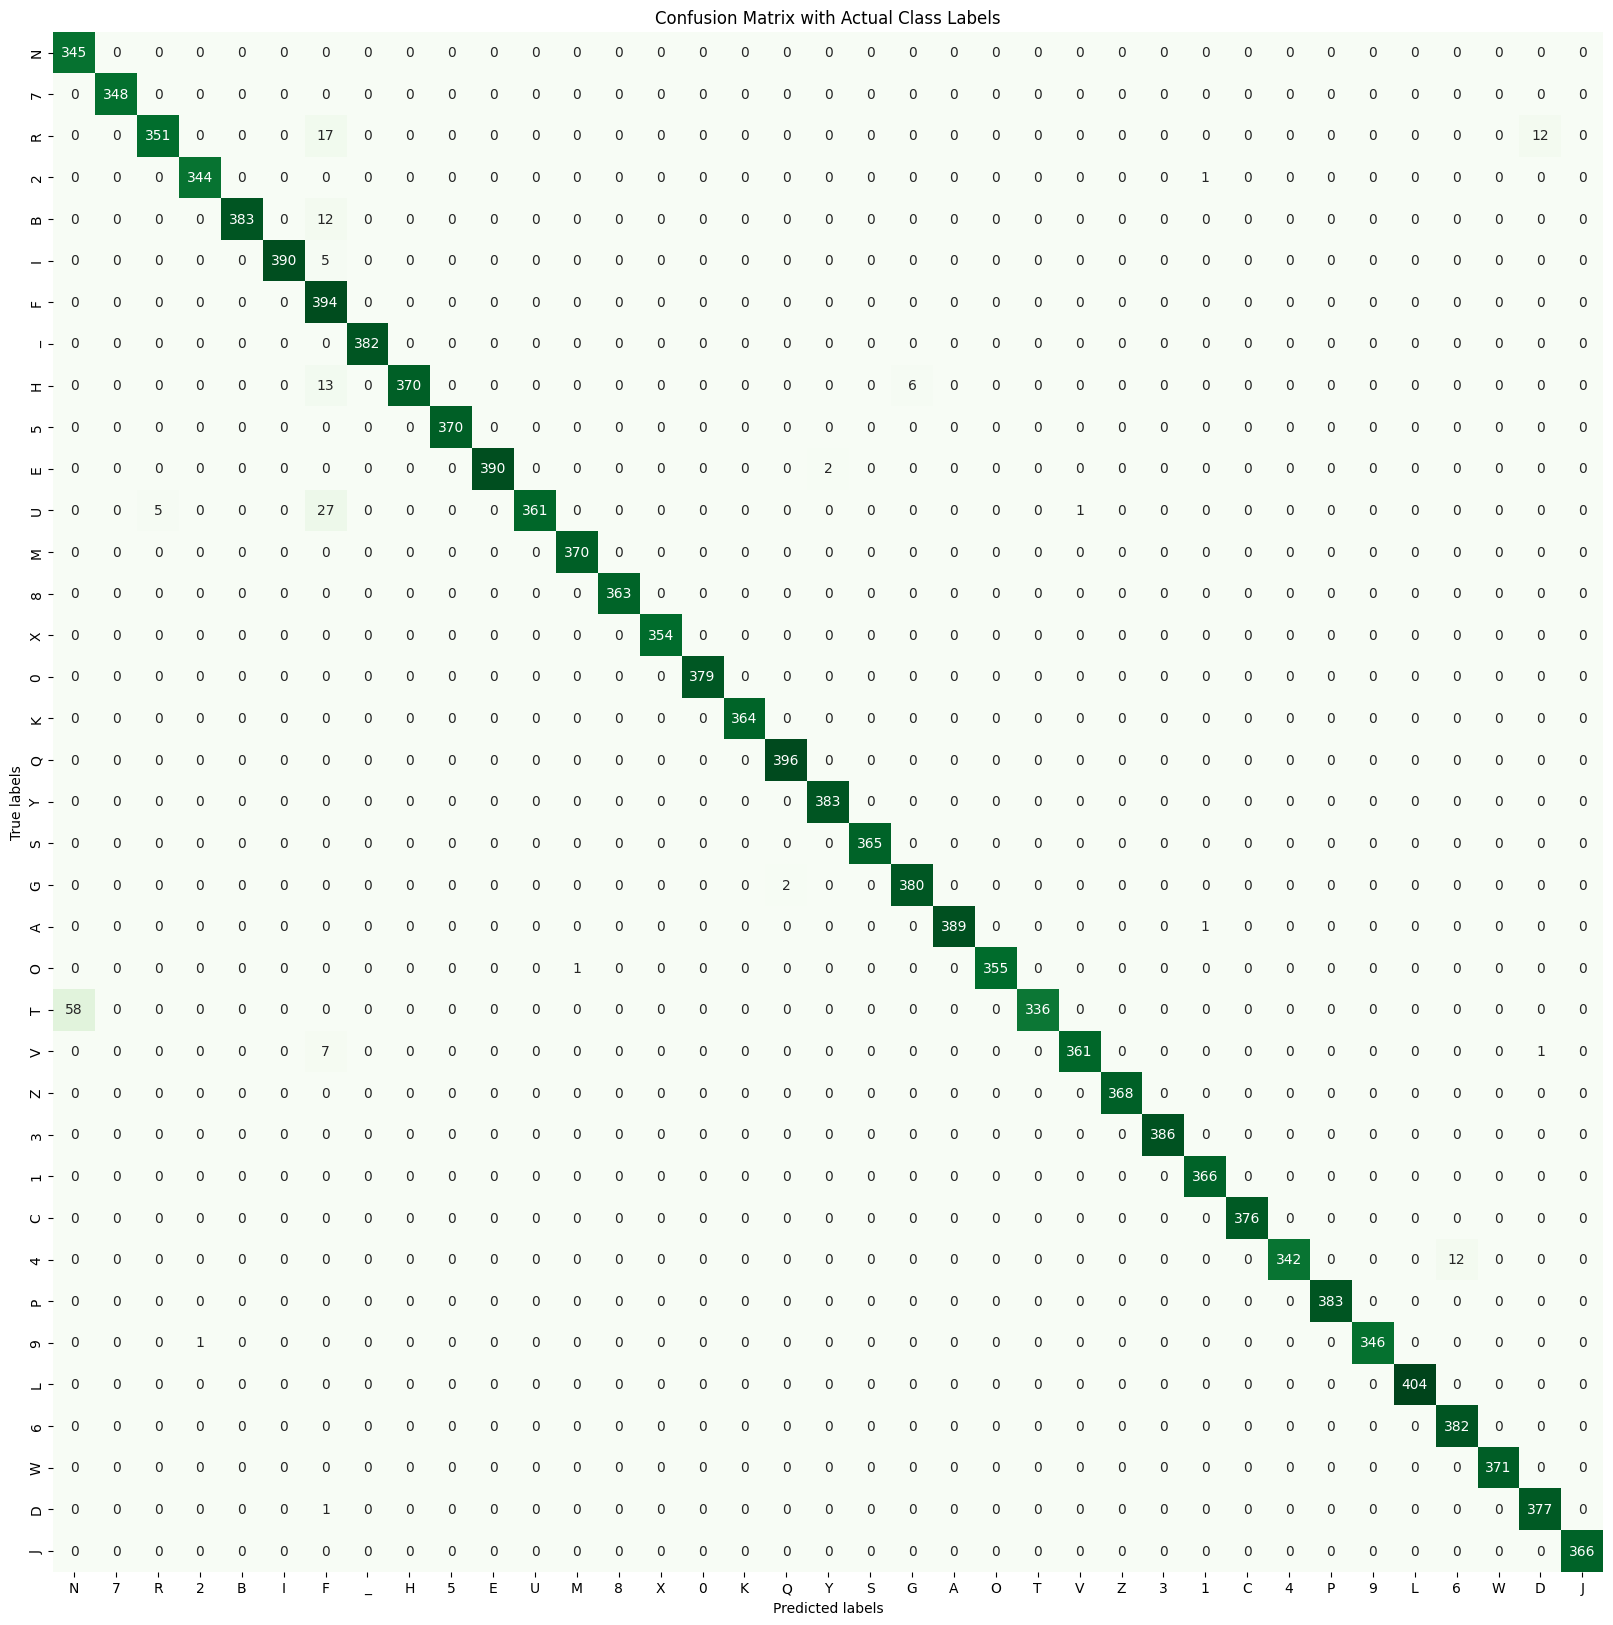
\includegraphics[width=0.55\textwidth]{Assets/confusion_matrix/EfficientNetB0.png}
    \caption{Confusion Matrix: EfficientNetB0}
    \vspace{1.5cm}
    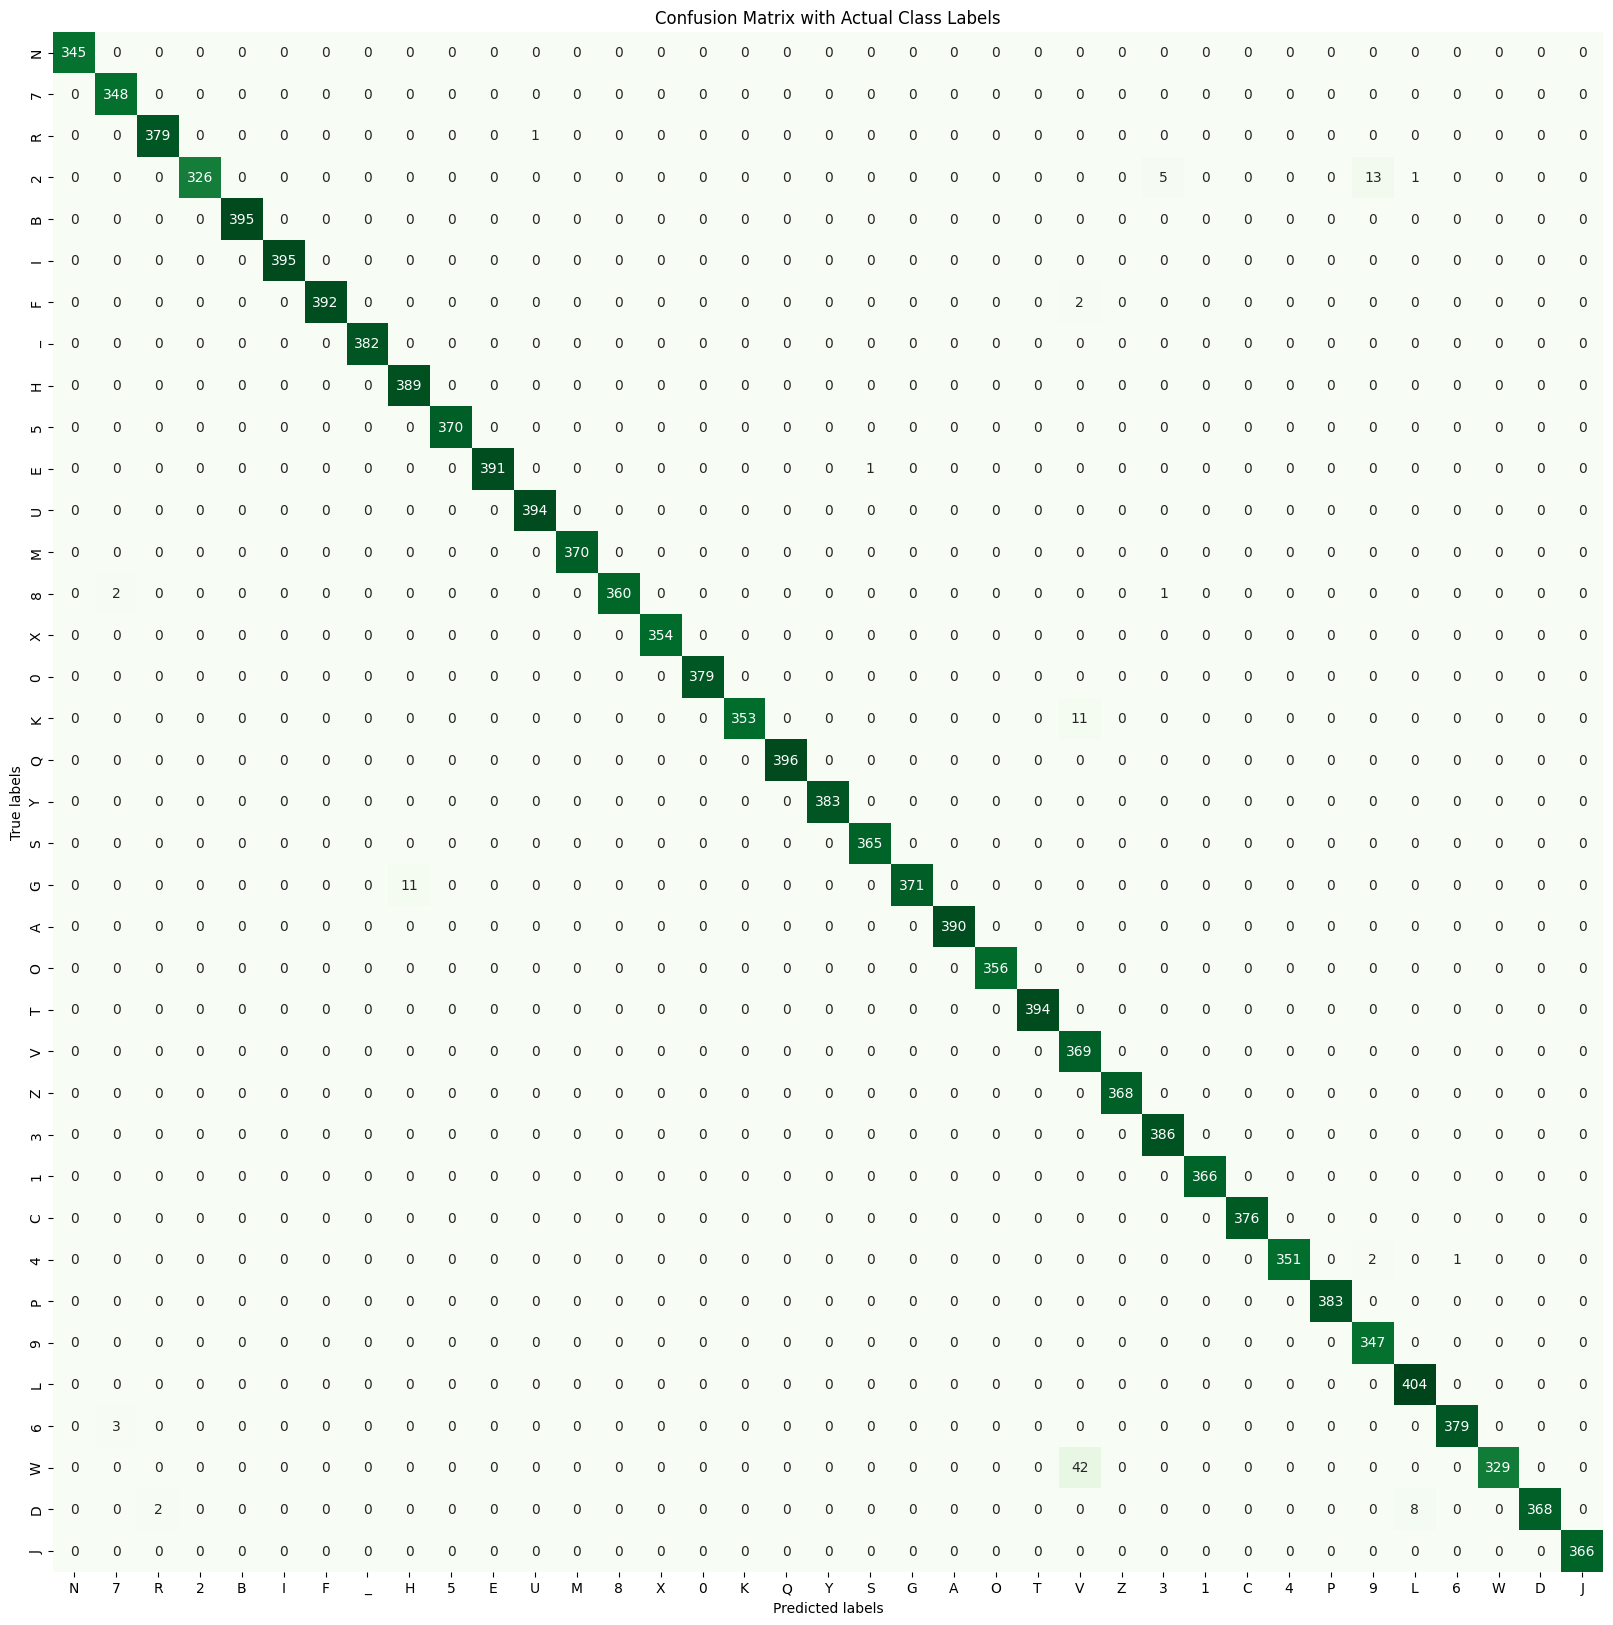
\includegraphics[width=0.55\textwidth]{Assets/confusion_matrix/efficientnetv2.png}
    \caption{Confusion Matrix: EfficientNetB1}
\end{figure}

\newpage

\begin{figure}[h!]
    \centering
    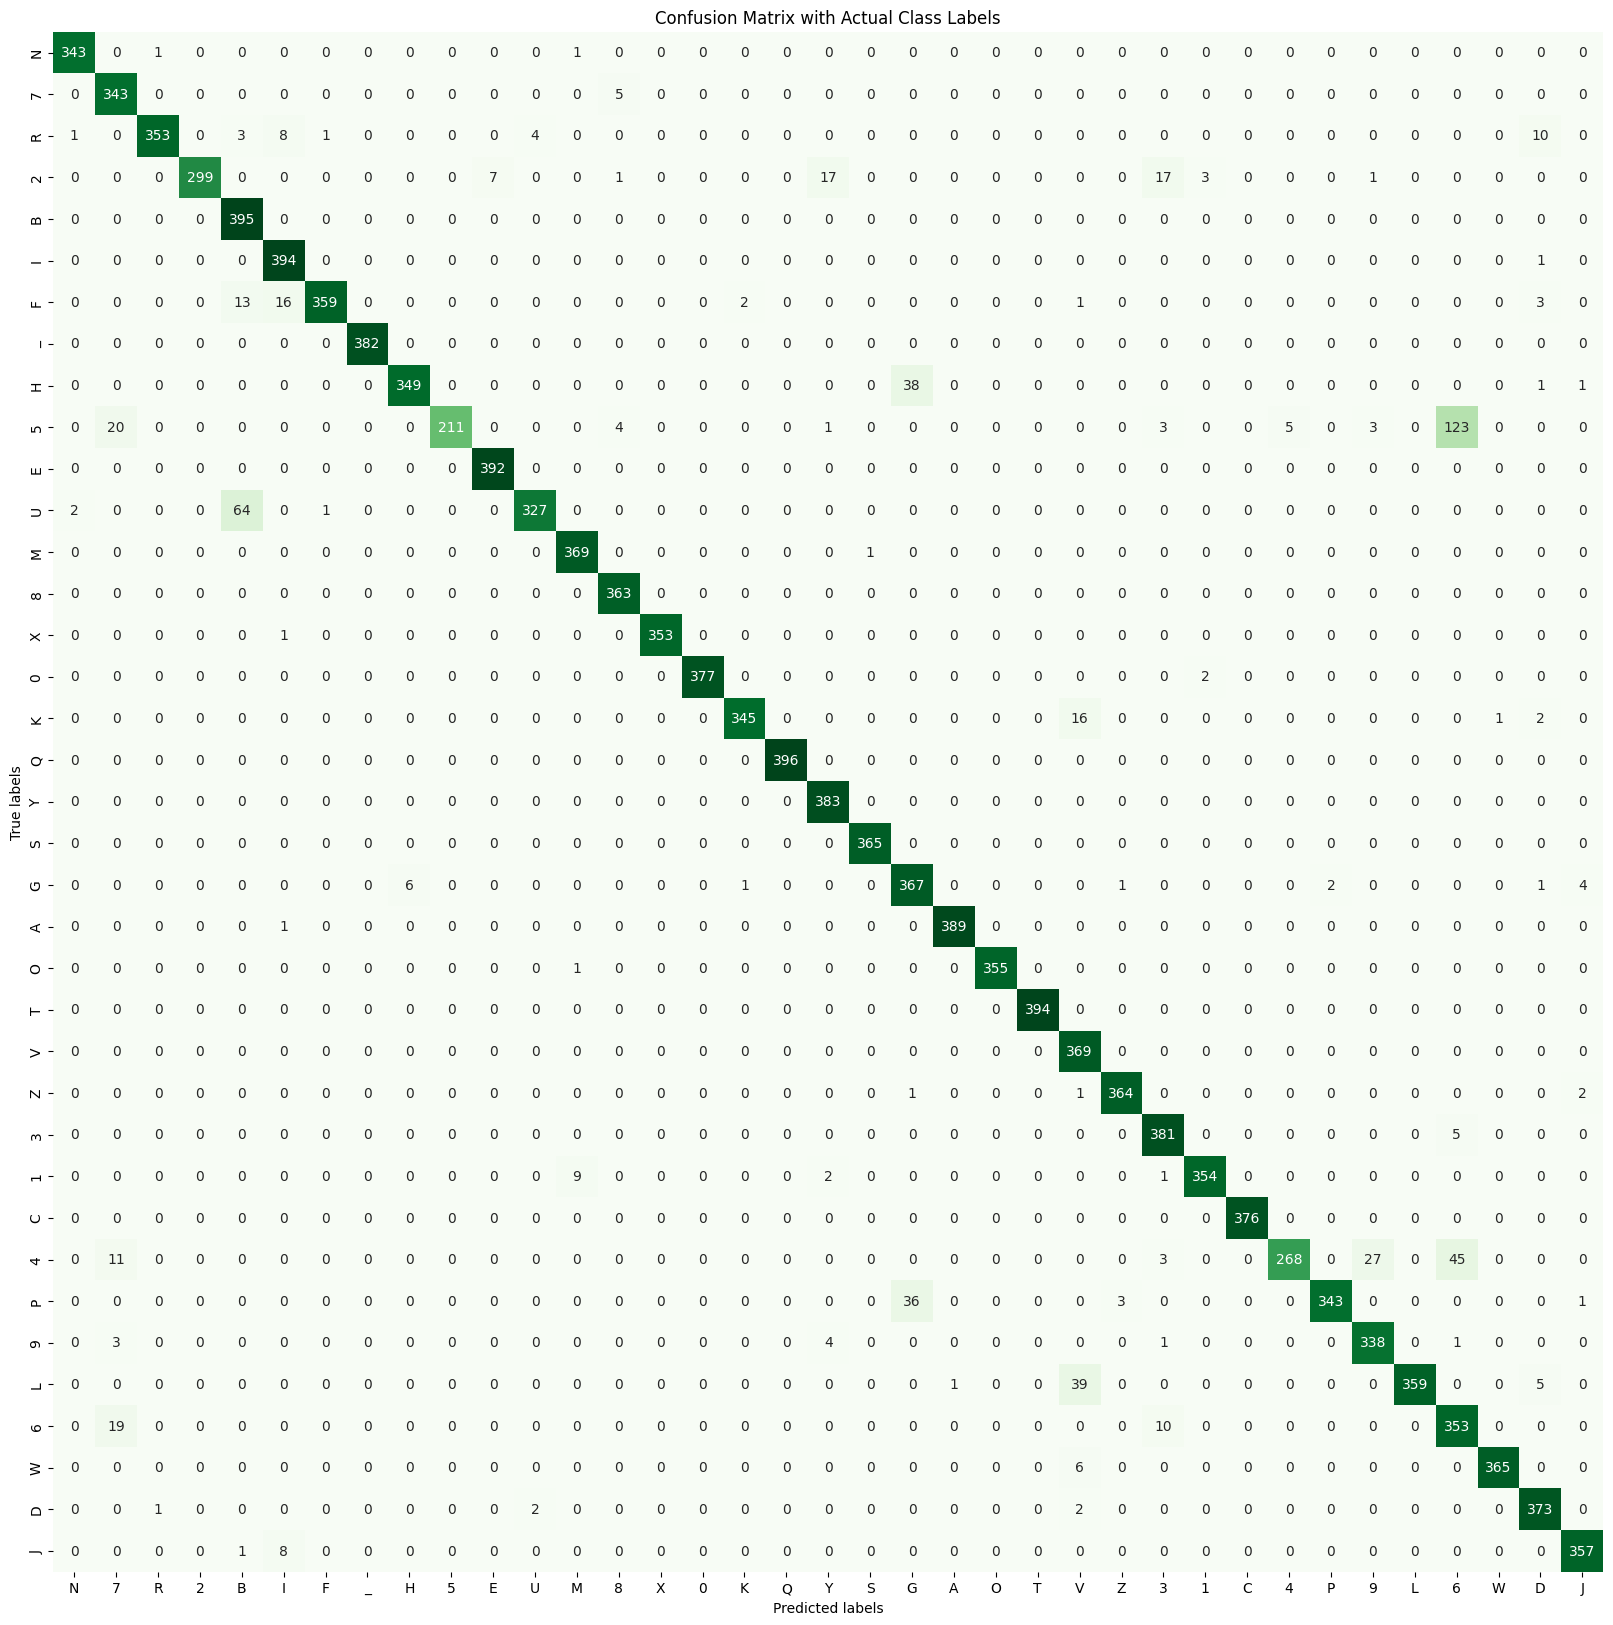
\includegraphics[width=0.55\textwidth]{Assets/confusion_matrix/EfficientNetV2L.png}
    \caption{Confusion Matrix: EfficientNetV2L}
    \vspace{1.5cm}
    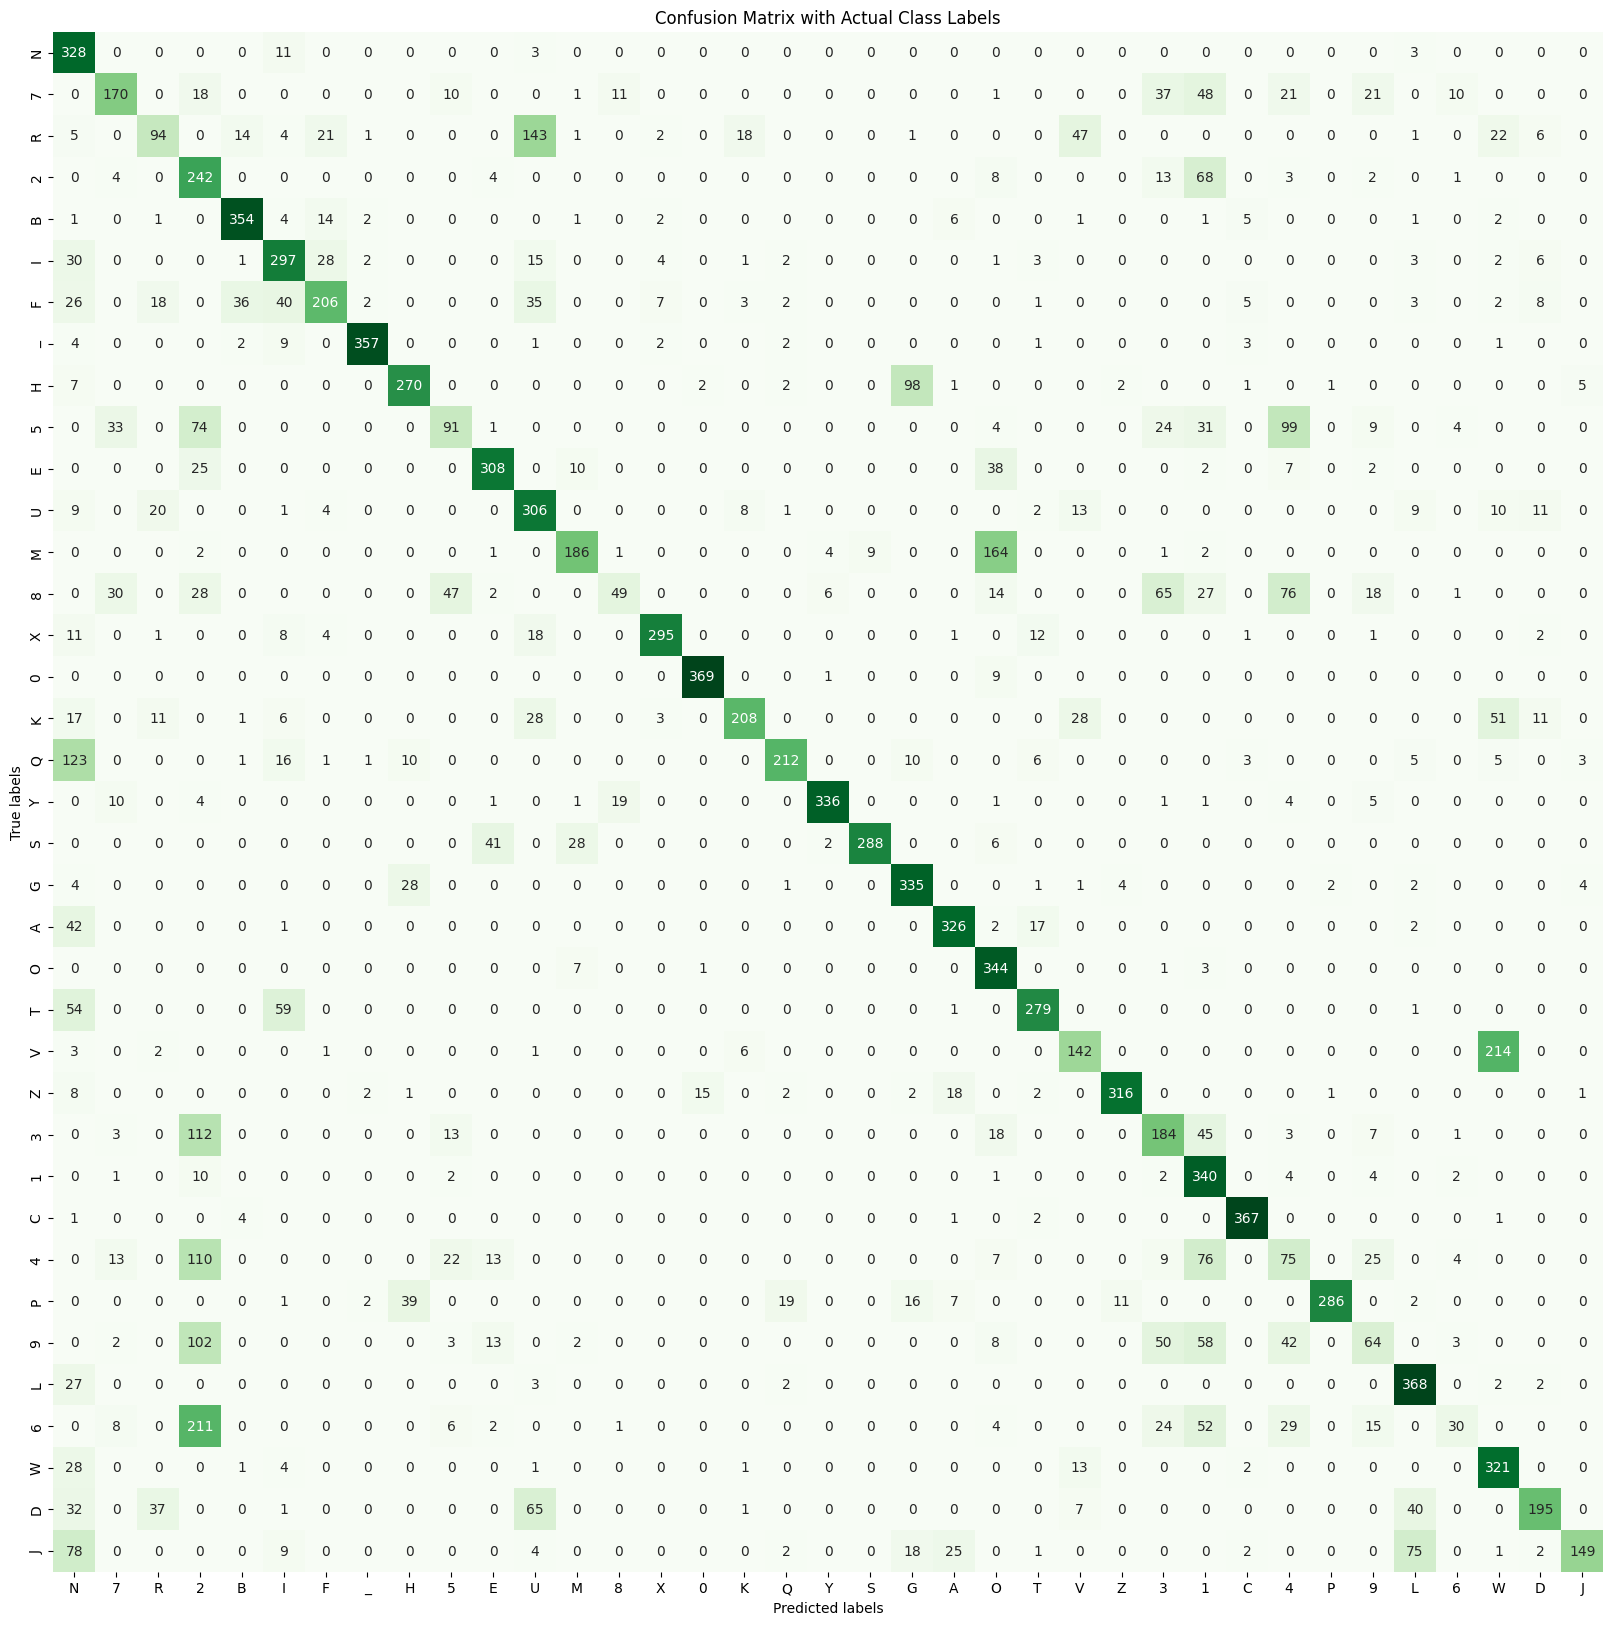
\includegraphics[width=0.55\textwidth]{Assets/confusion_matrix/MOBILENETV2.png}
    \caption{Confusion Matrix: MOBILENETV2}
\end{figure}

\newpage

\begin{figure}[h!]
    \centering
    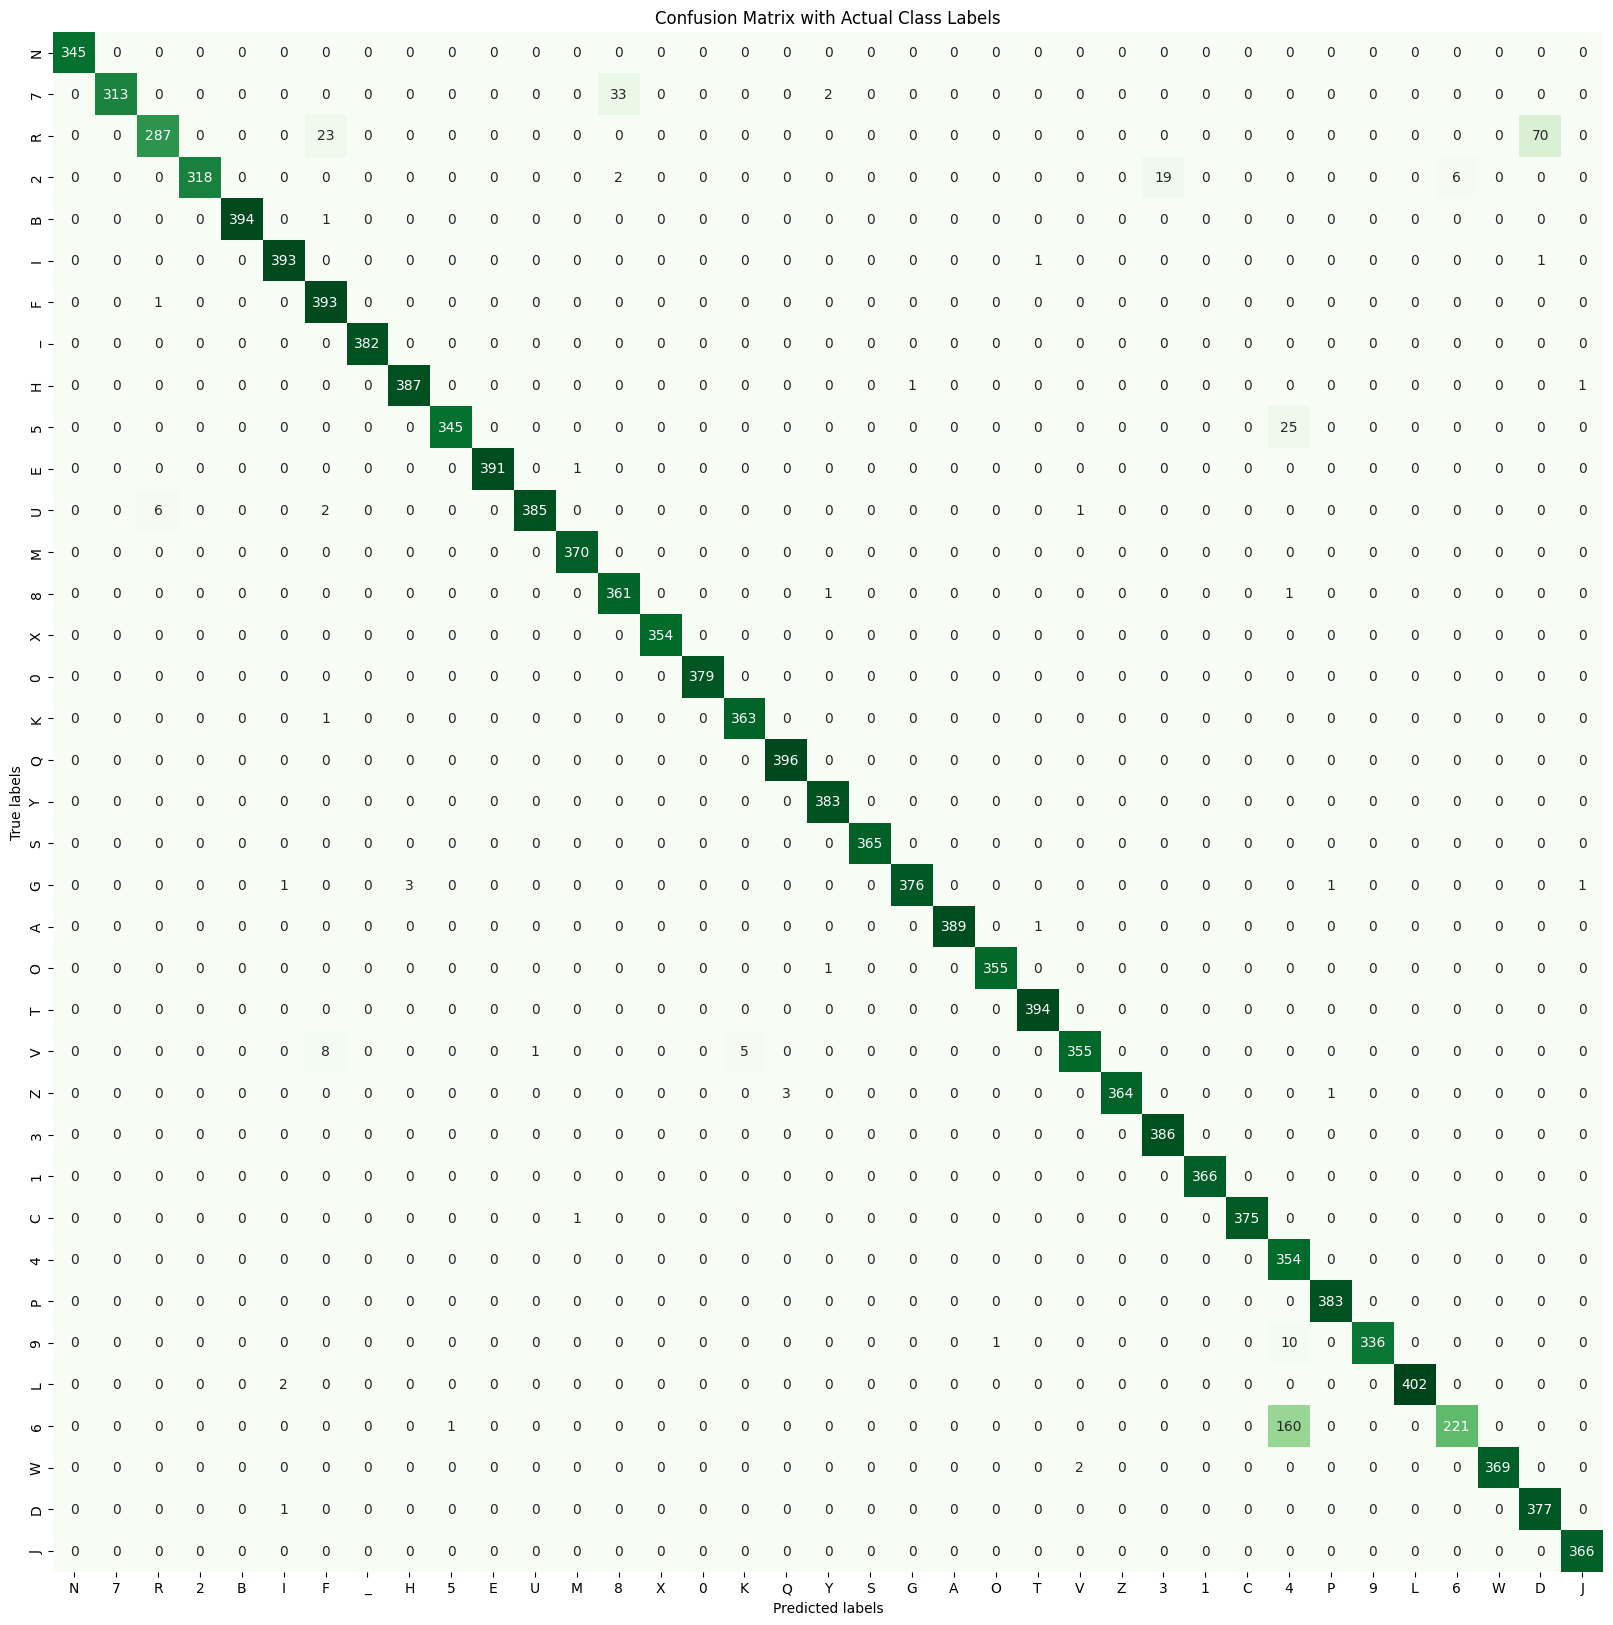
\includegraphics[width=0.55\textwidth]{Assets/confusion_matrix/MobileNetV3Large.png}
    \caption{Confusion Matrix: MobileNetV3Large}
    \vspace{1.5cm}
    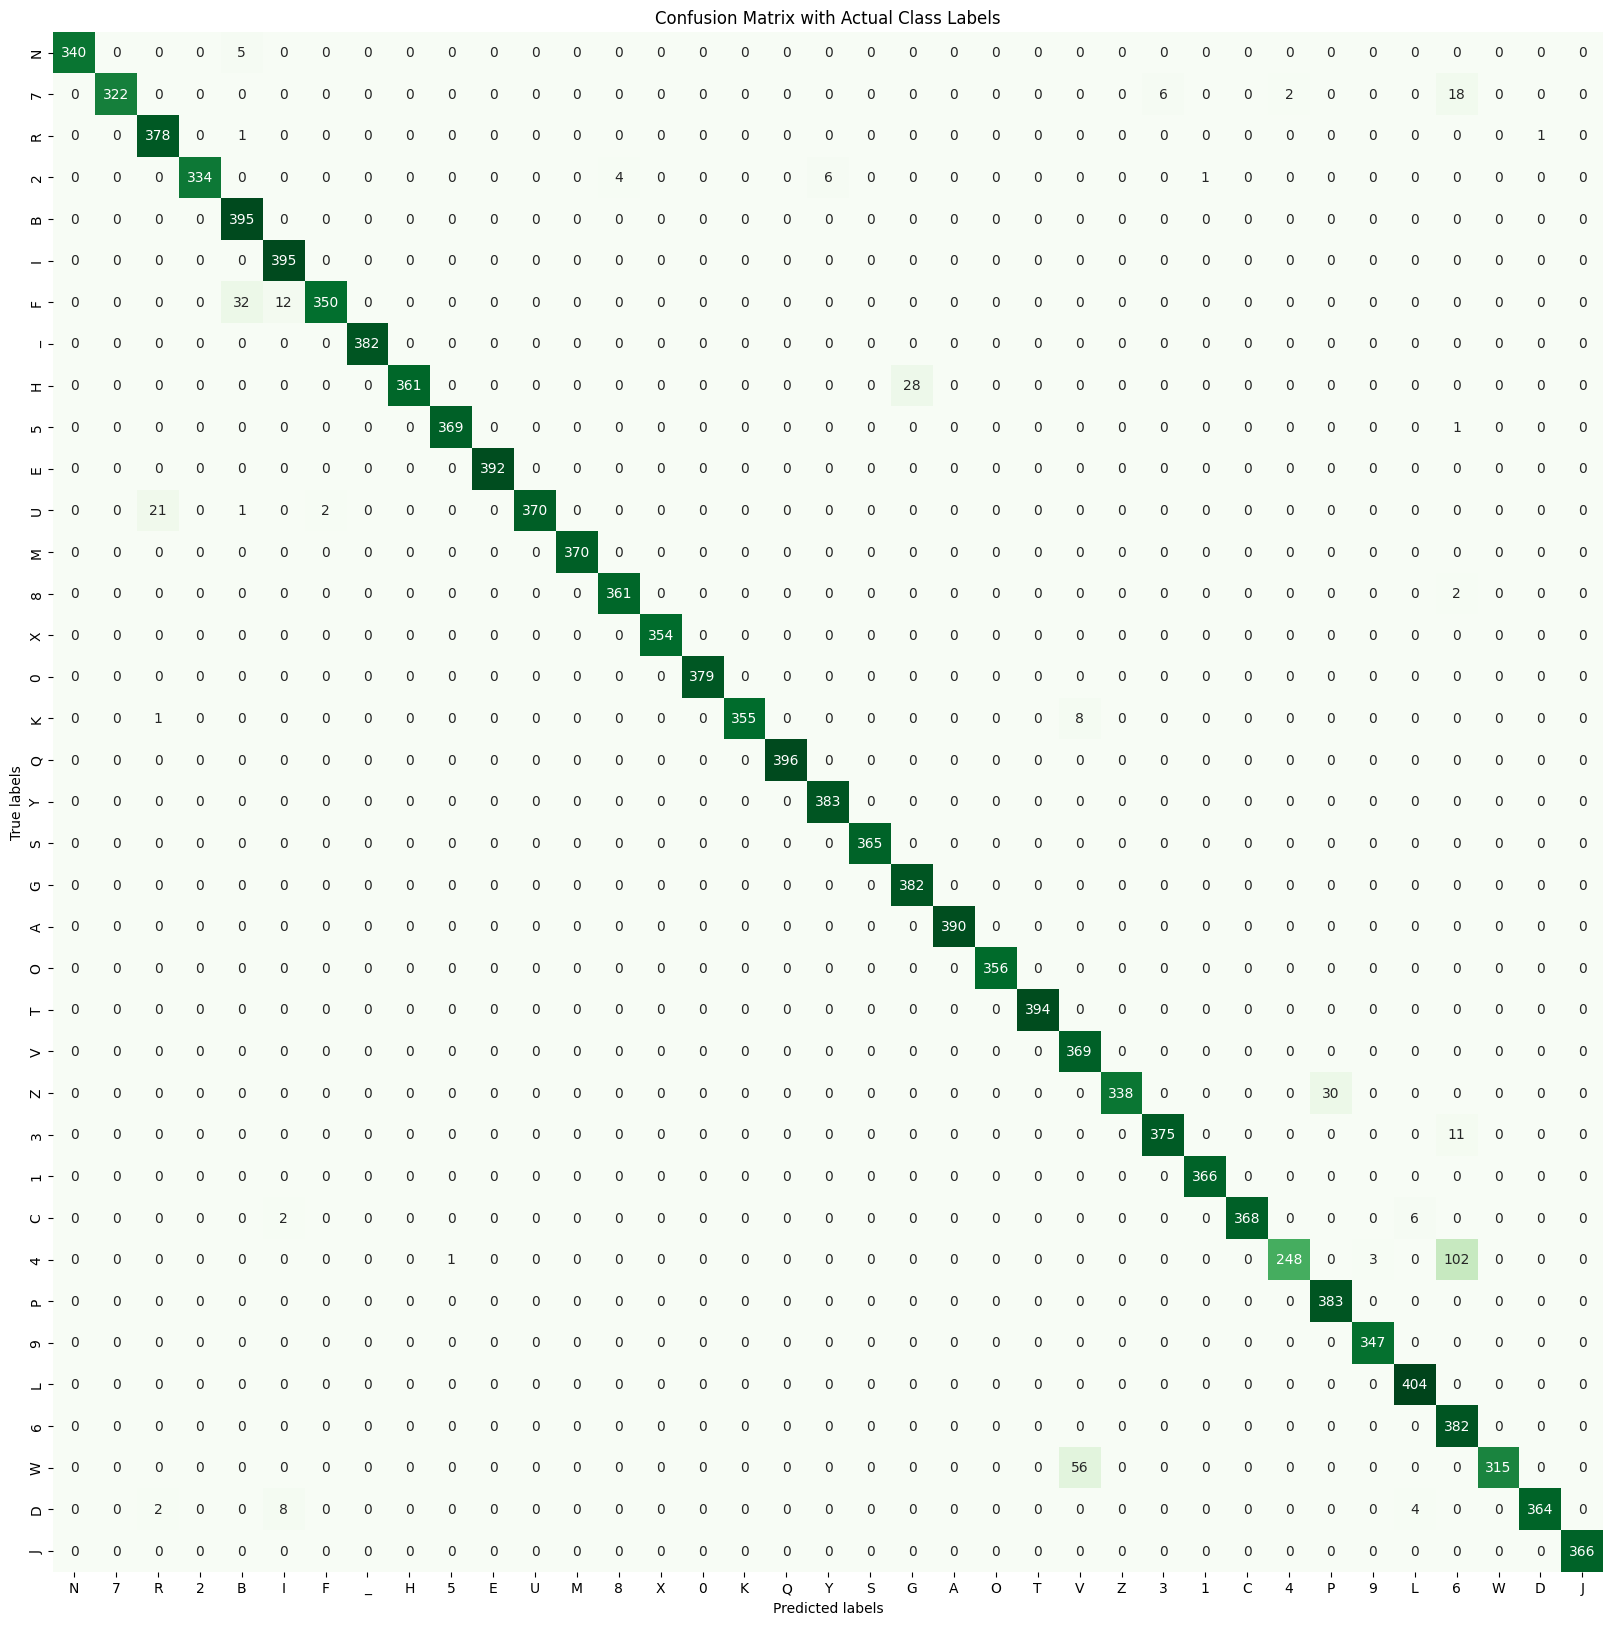
\includegraphics[width=0.55\textwidth]{Assets/confusion_matrix/ResNet50.png}
    \caption{Confusion Matrix: ResNet50}
\end{figure}

\newpage

\begin{figure}[h!]
    \centering
    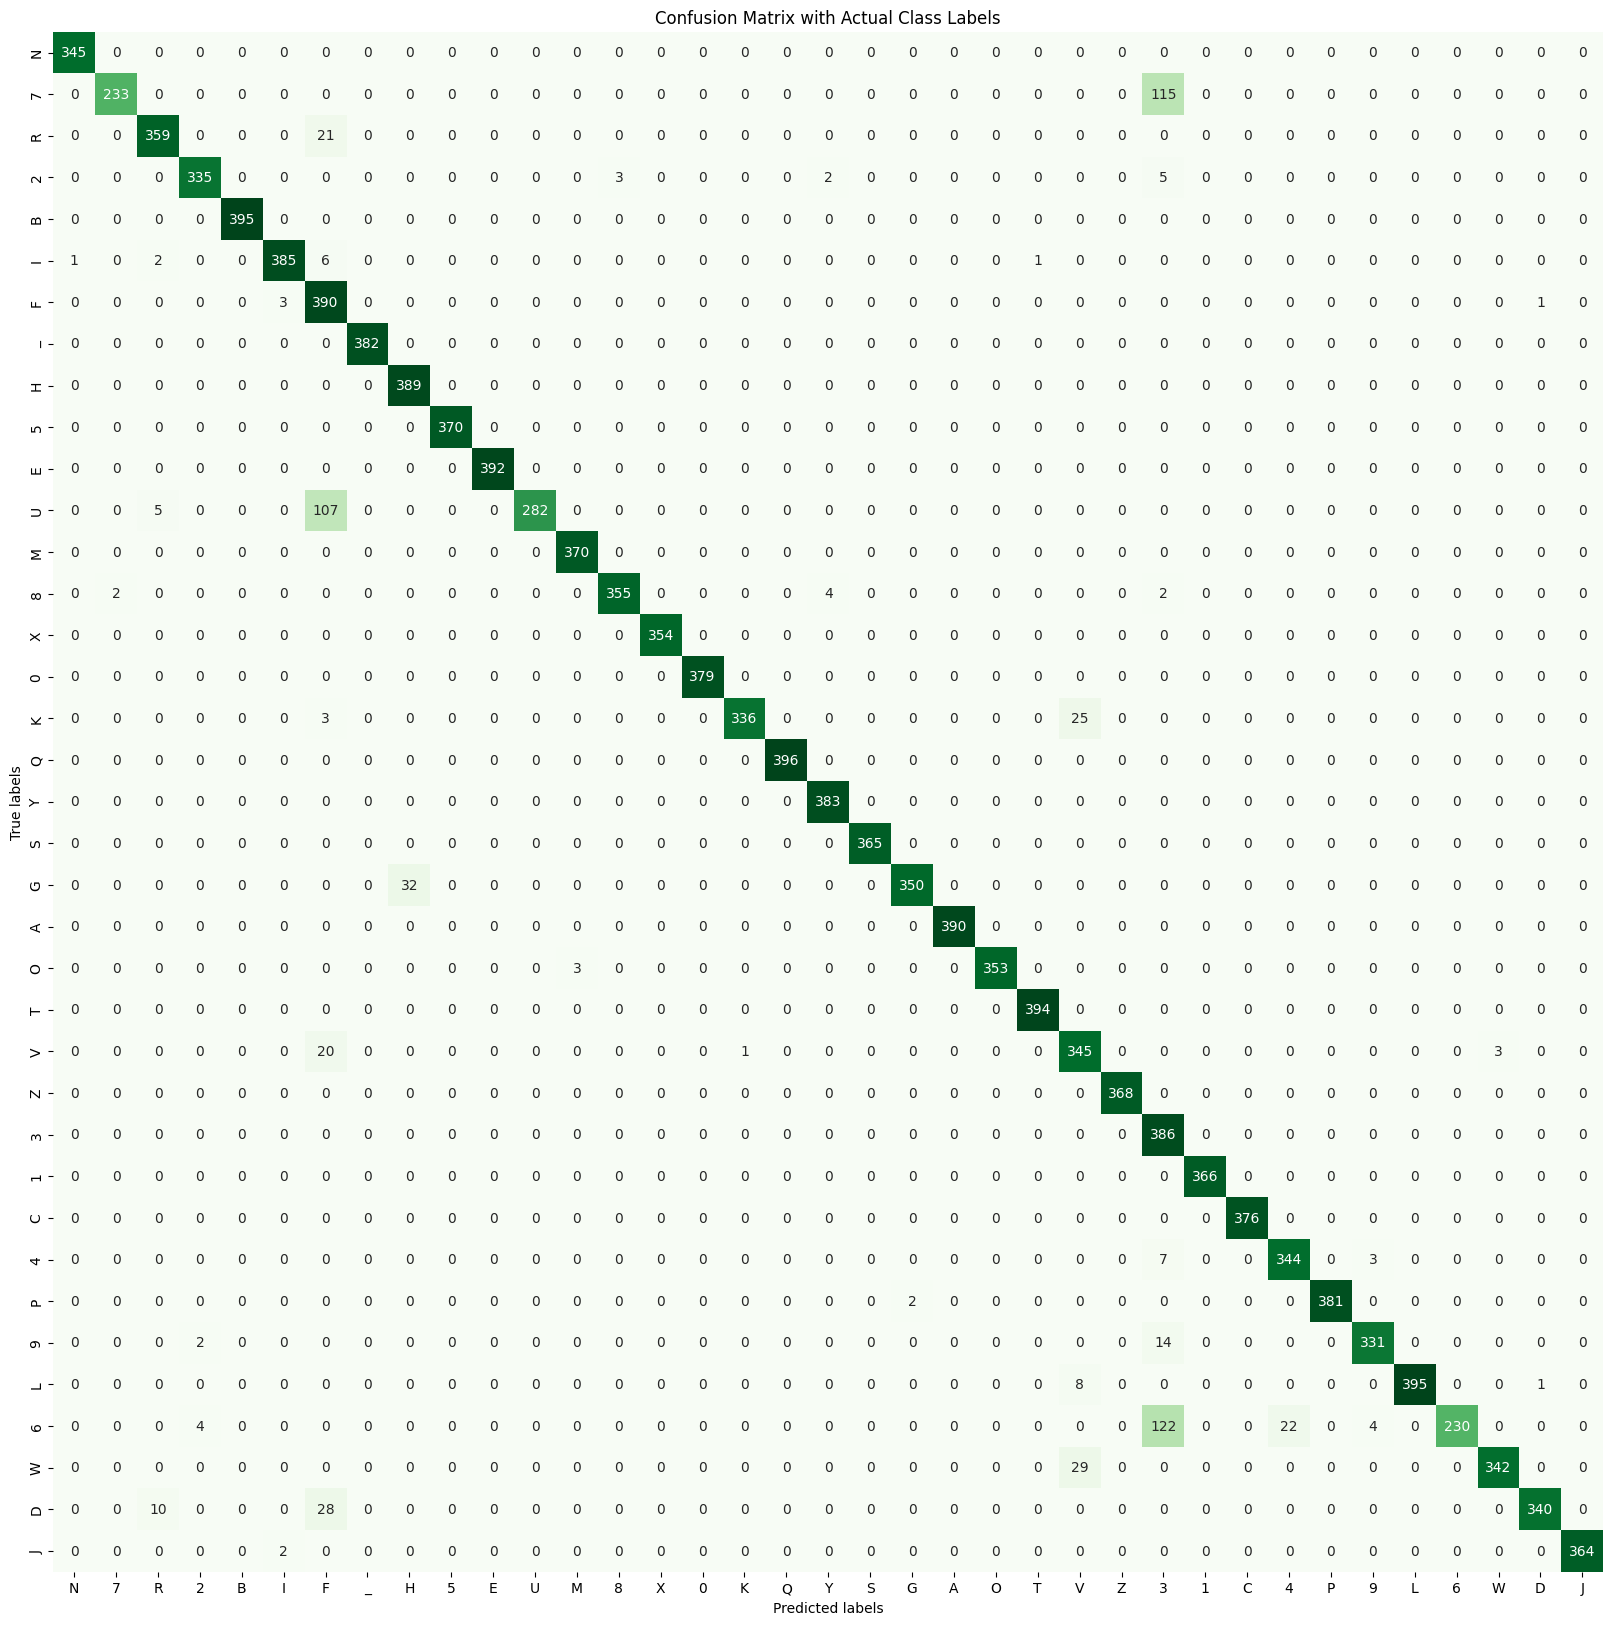
\includegraphics[width=0.55\textwidth]{Assets/confusion_matrix/RESNET101.png}
    \caption{Confusion Matrix: RESNET101}
    \vspace{1.5cm}
    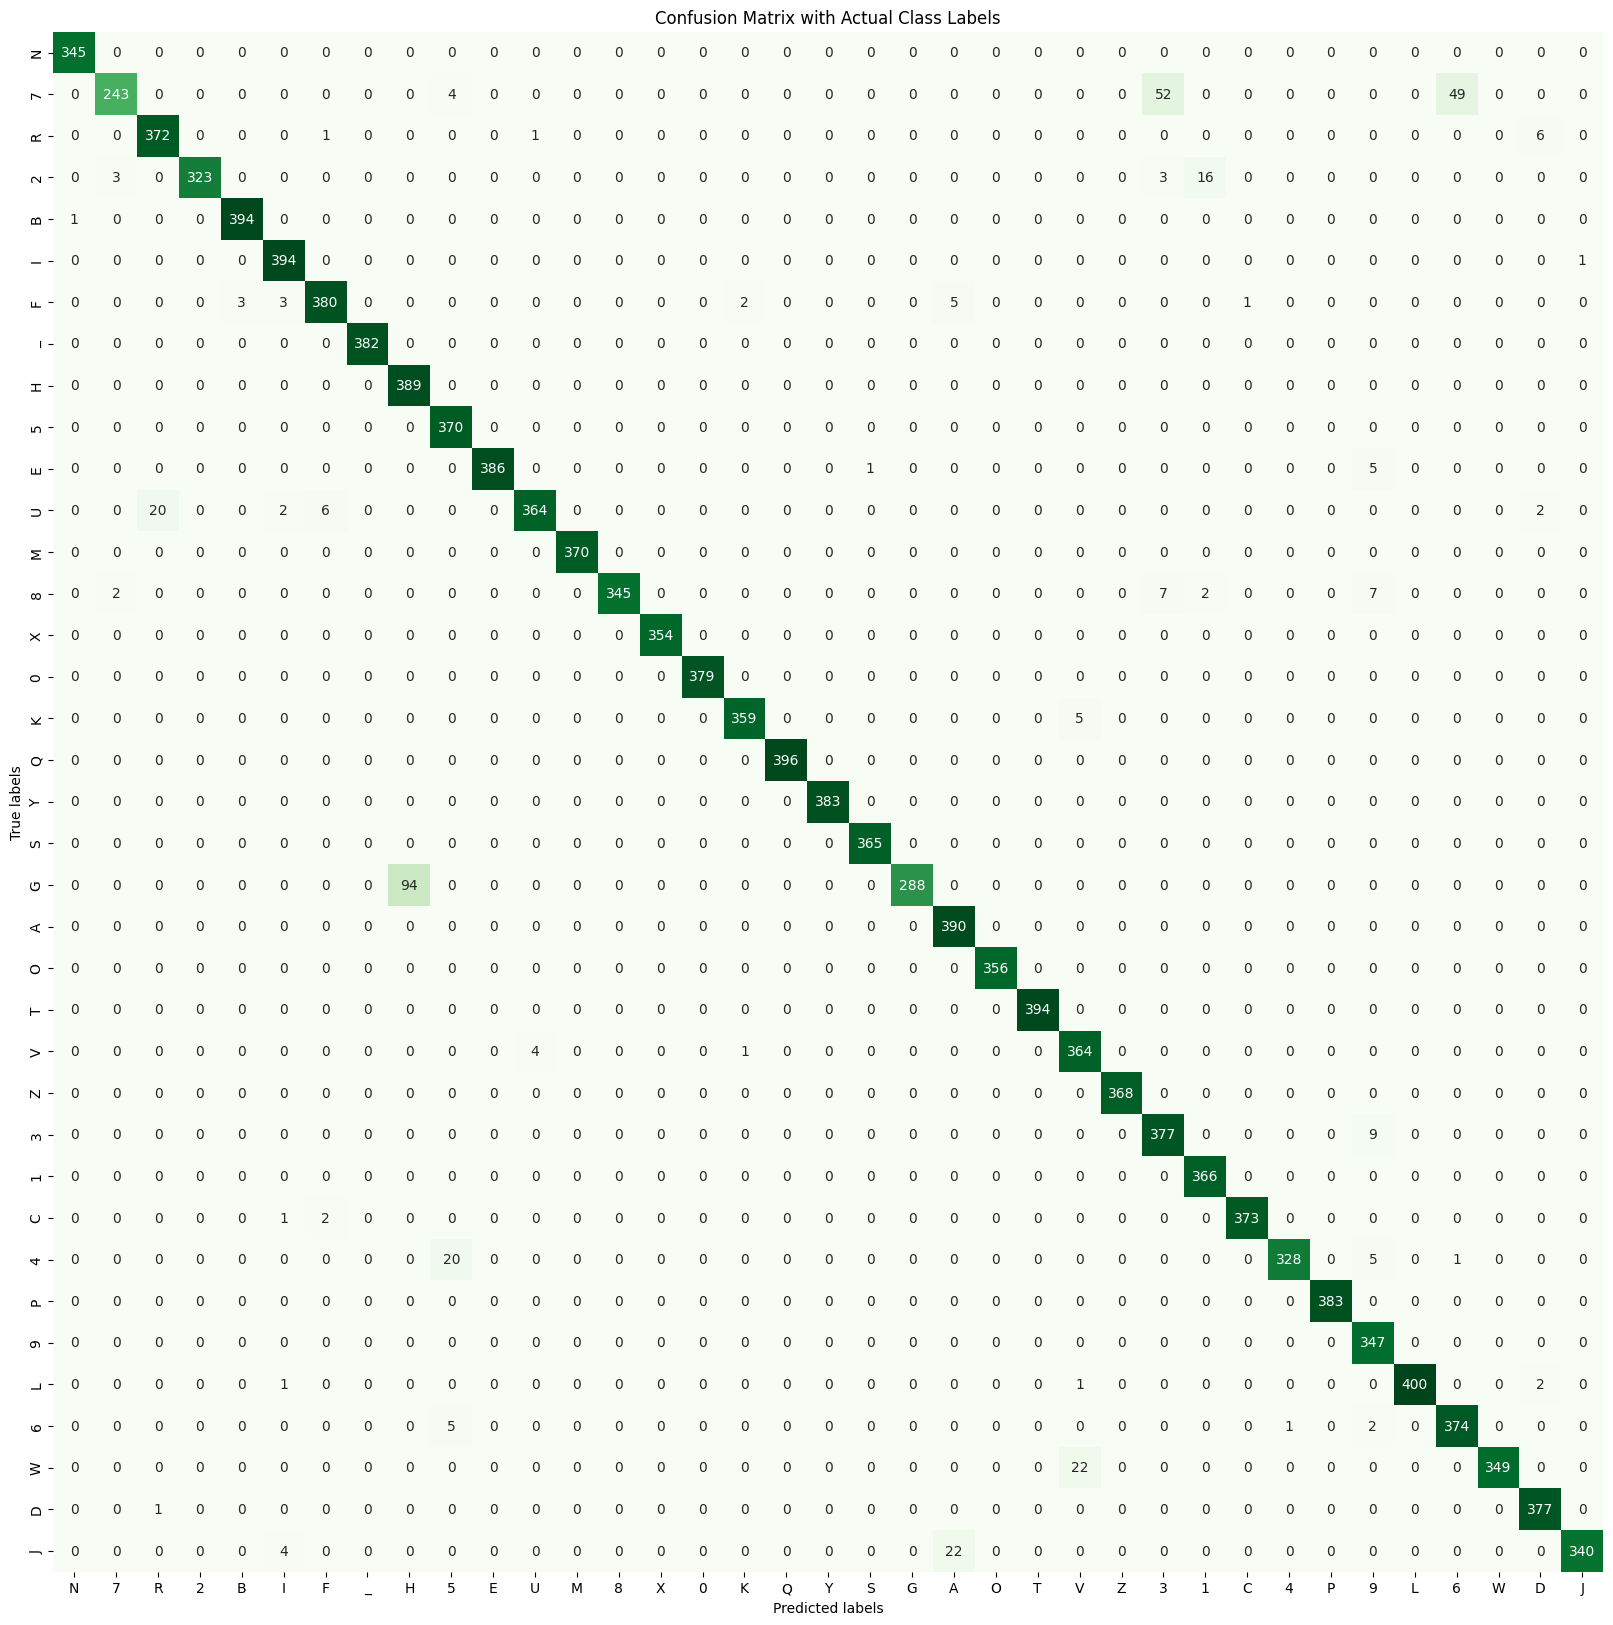
\includegraphics[width=0.55\textwidth]{Assets/confusion_matrix/RESNET152.png}
    \caption{Confusion Matrix: RESNET152}
\end{figure}

\newpage

\begin{figure}[h!]
    \centering
    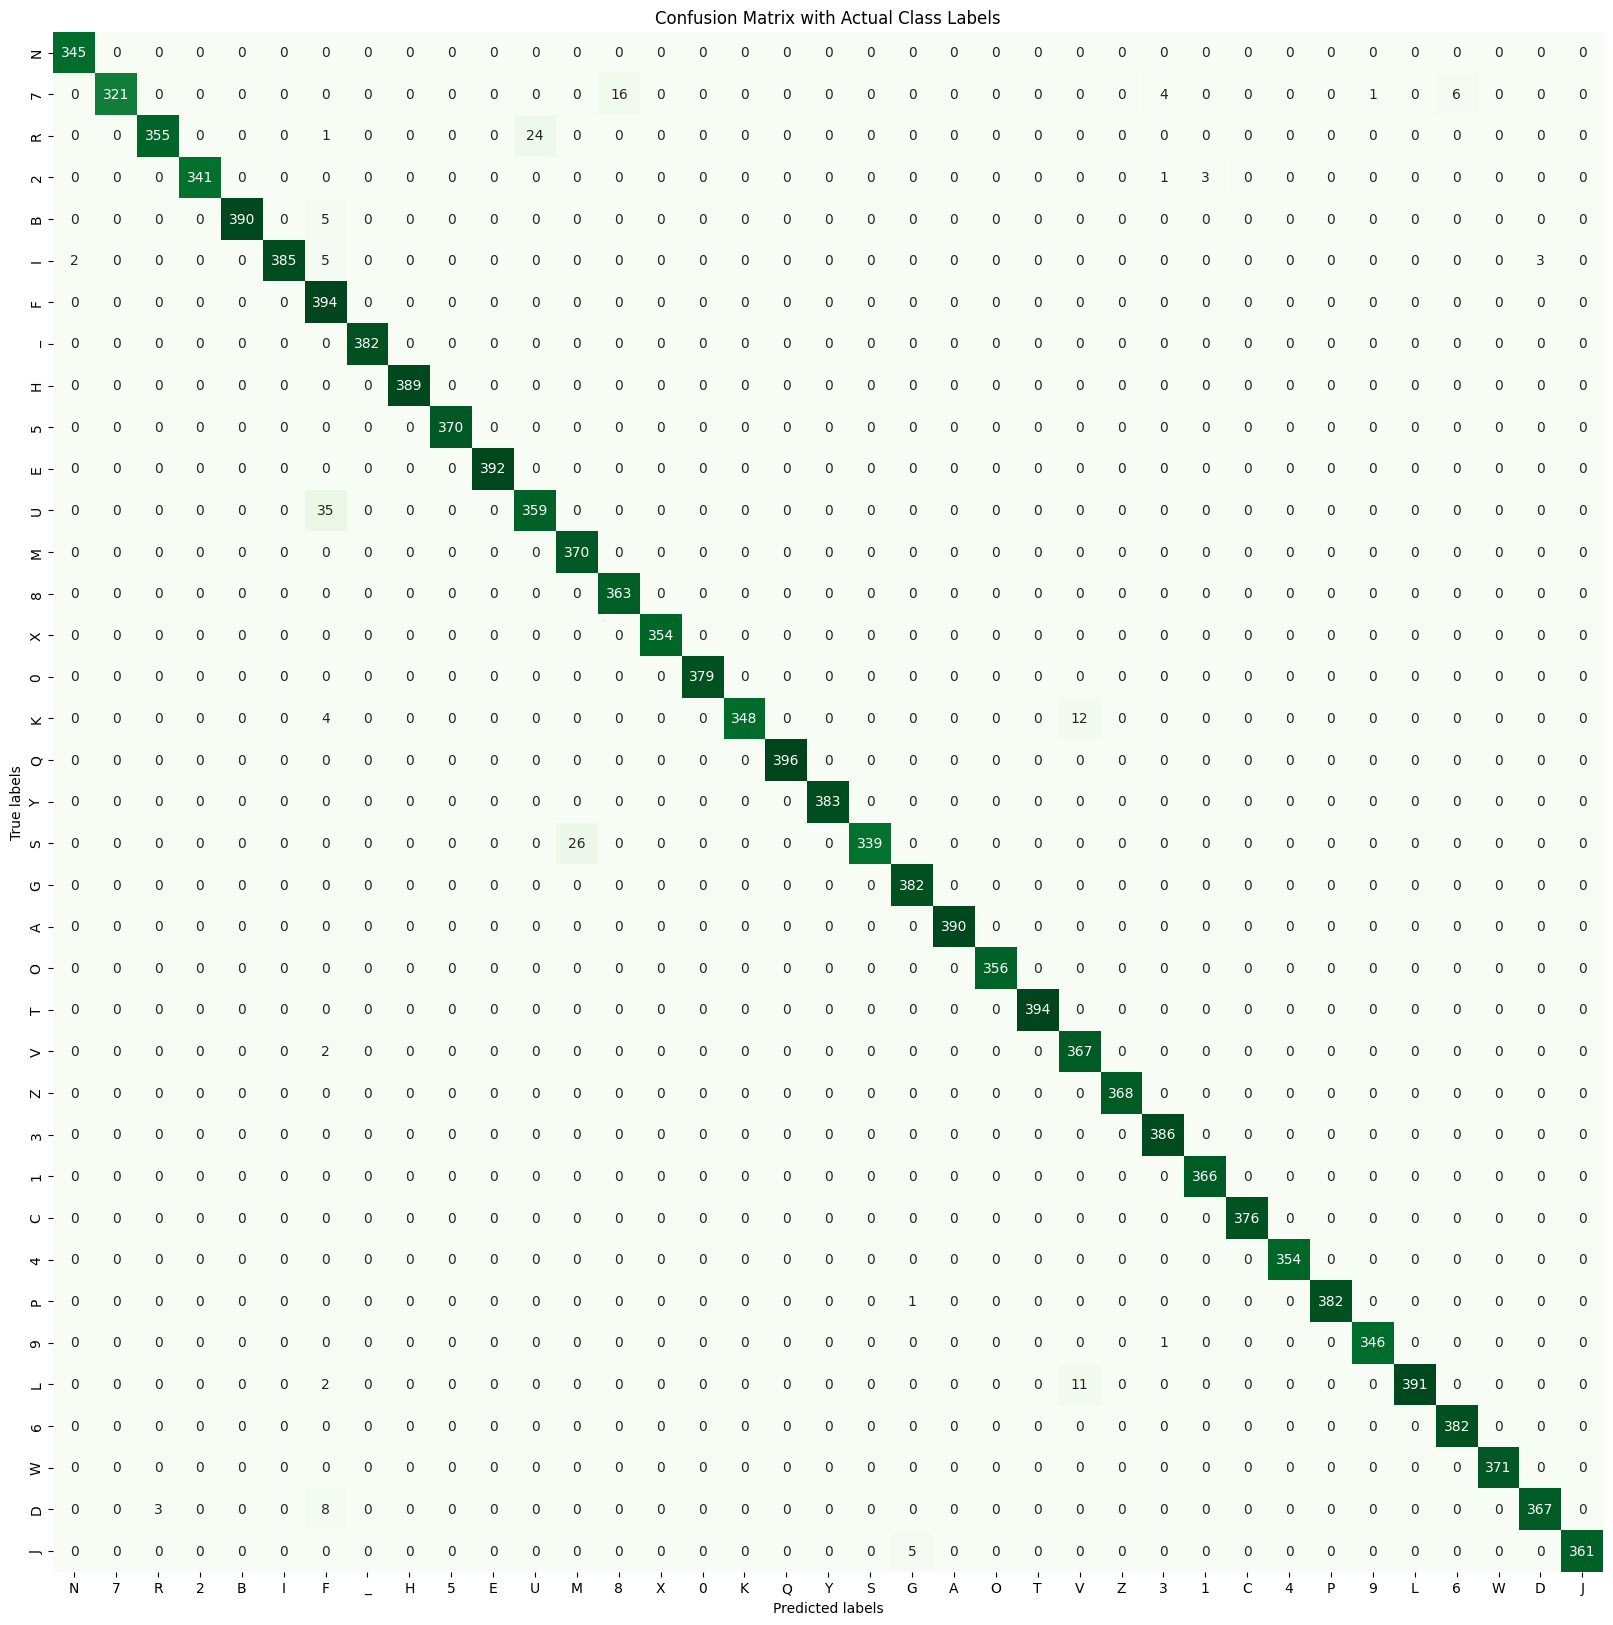
\includegraphics[width=0.55\textwidth]{Assets/confusion_matrix/vgg16.png}
    \caption{Confusion Matrix: VGG16}
    \vspace{1.5cm}
    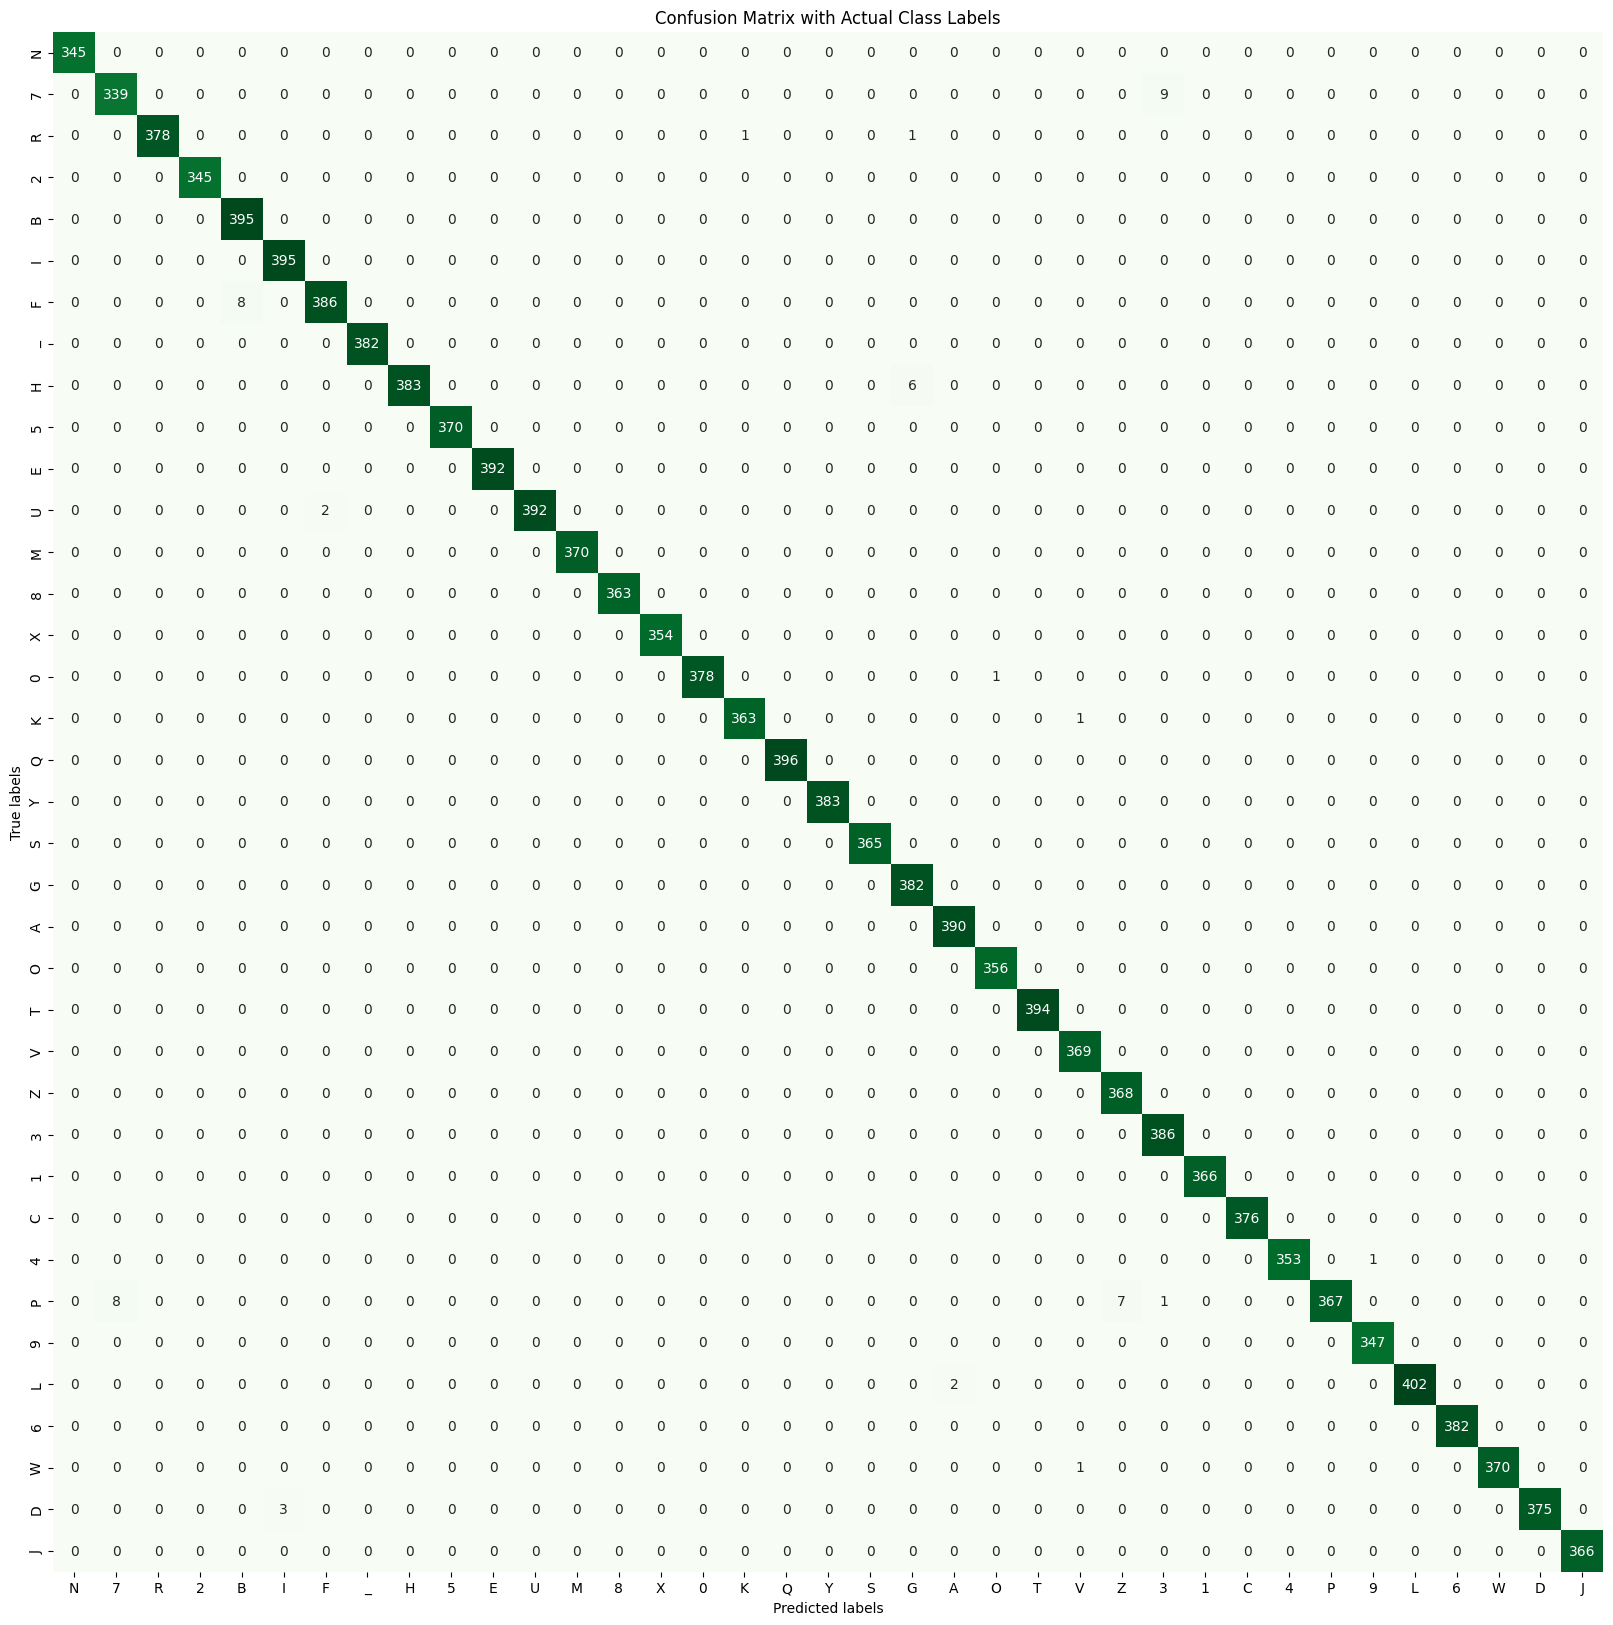
\includegraphics[width=0.55\textwidth]{Assets/confusion_matrix/CONVNEXT.png}
    \caption{Confusion Matrix: CONVNEXT}
\end{figure}


% \chapter*{Appendix-IV: t-SNE Plots}
\addcontentsline{toc}{chapter}{Appendix-IV: t-SNE Plots}

\noindent This appendix contains the t-SNE Plots for all models.

\begin{multicols}{2}
\centering

\setcounter{figure}{0} % Reset figure counter
\renewcommand{\thefigure}{2.\arabic{figure}} % Prefix figures with "2."

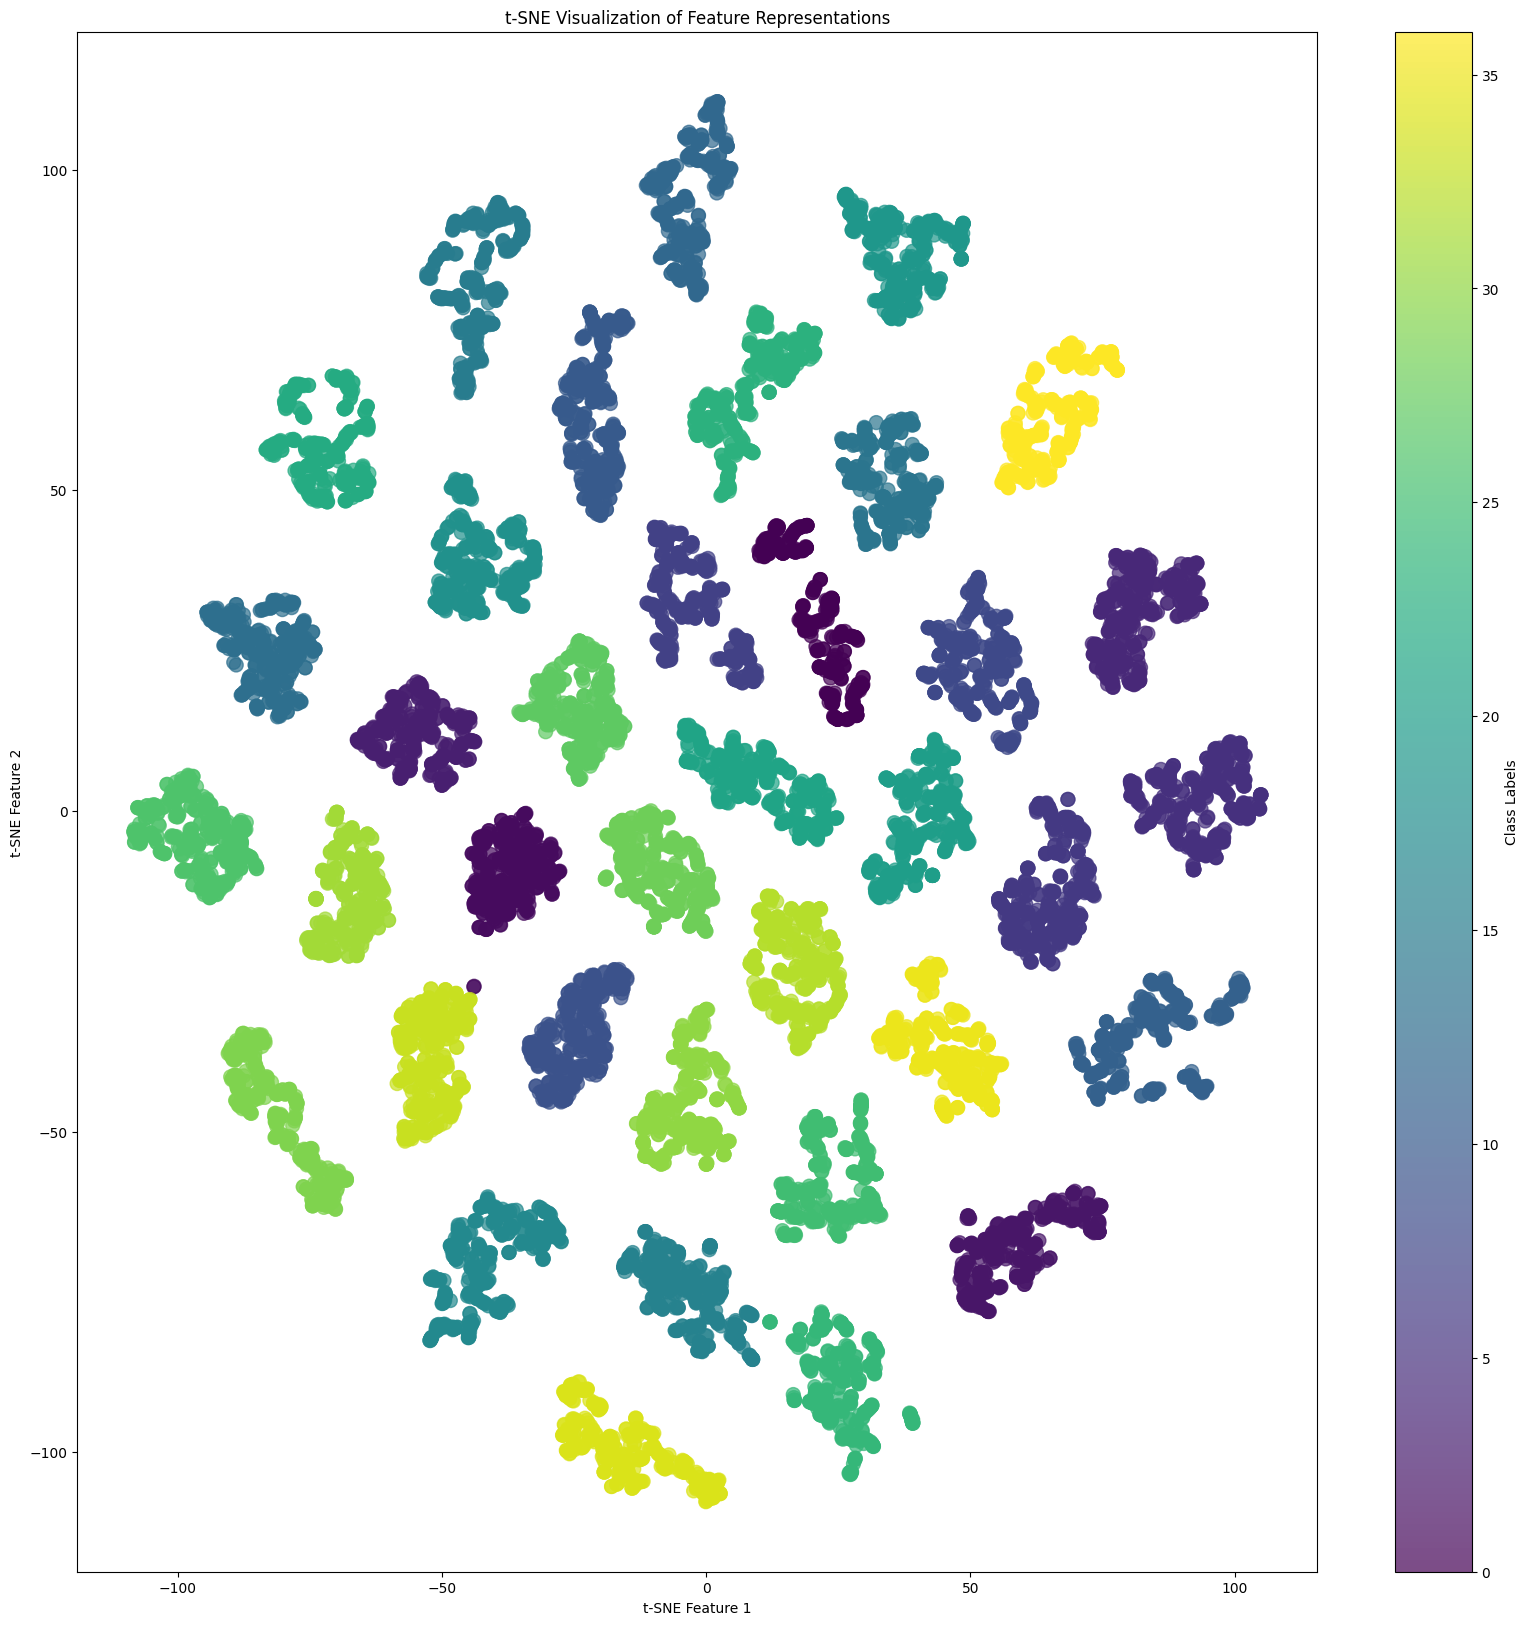
\includegraphics[width=0.41\textwidth]{Assets/tSNE/vgg19.png}
\captionof{figure}{VGG19}

\vspace{0.5cm}

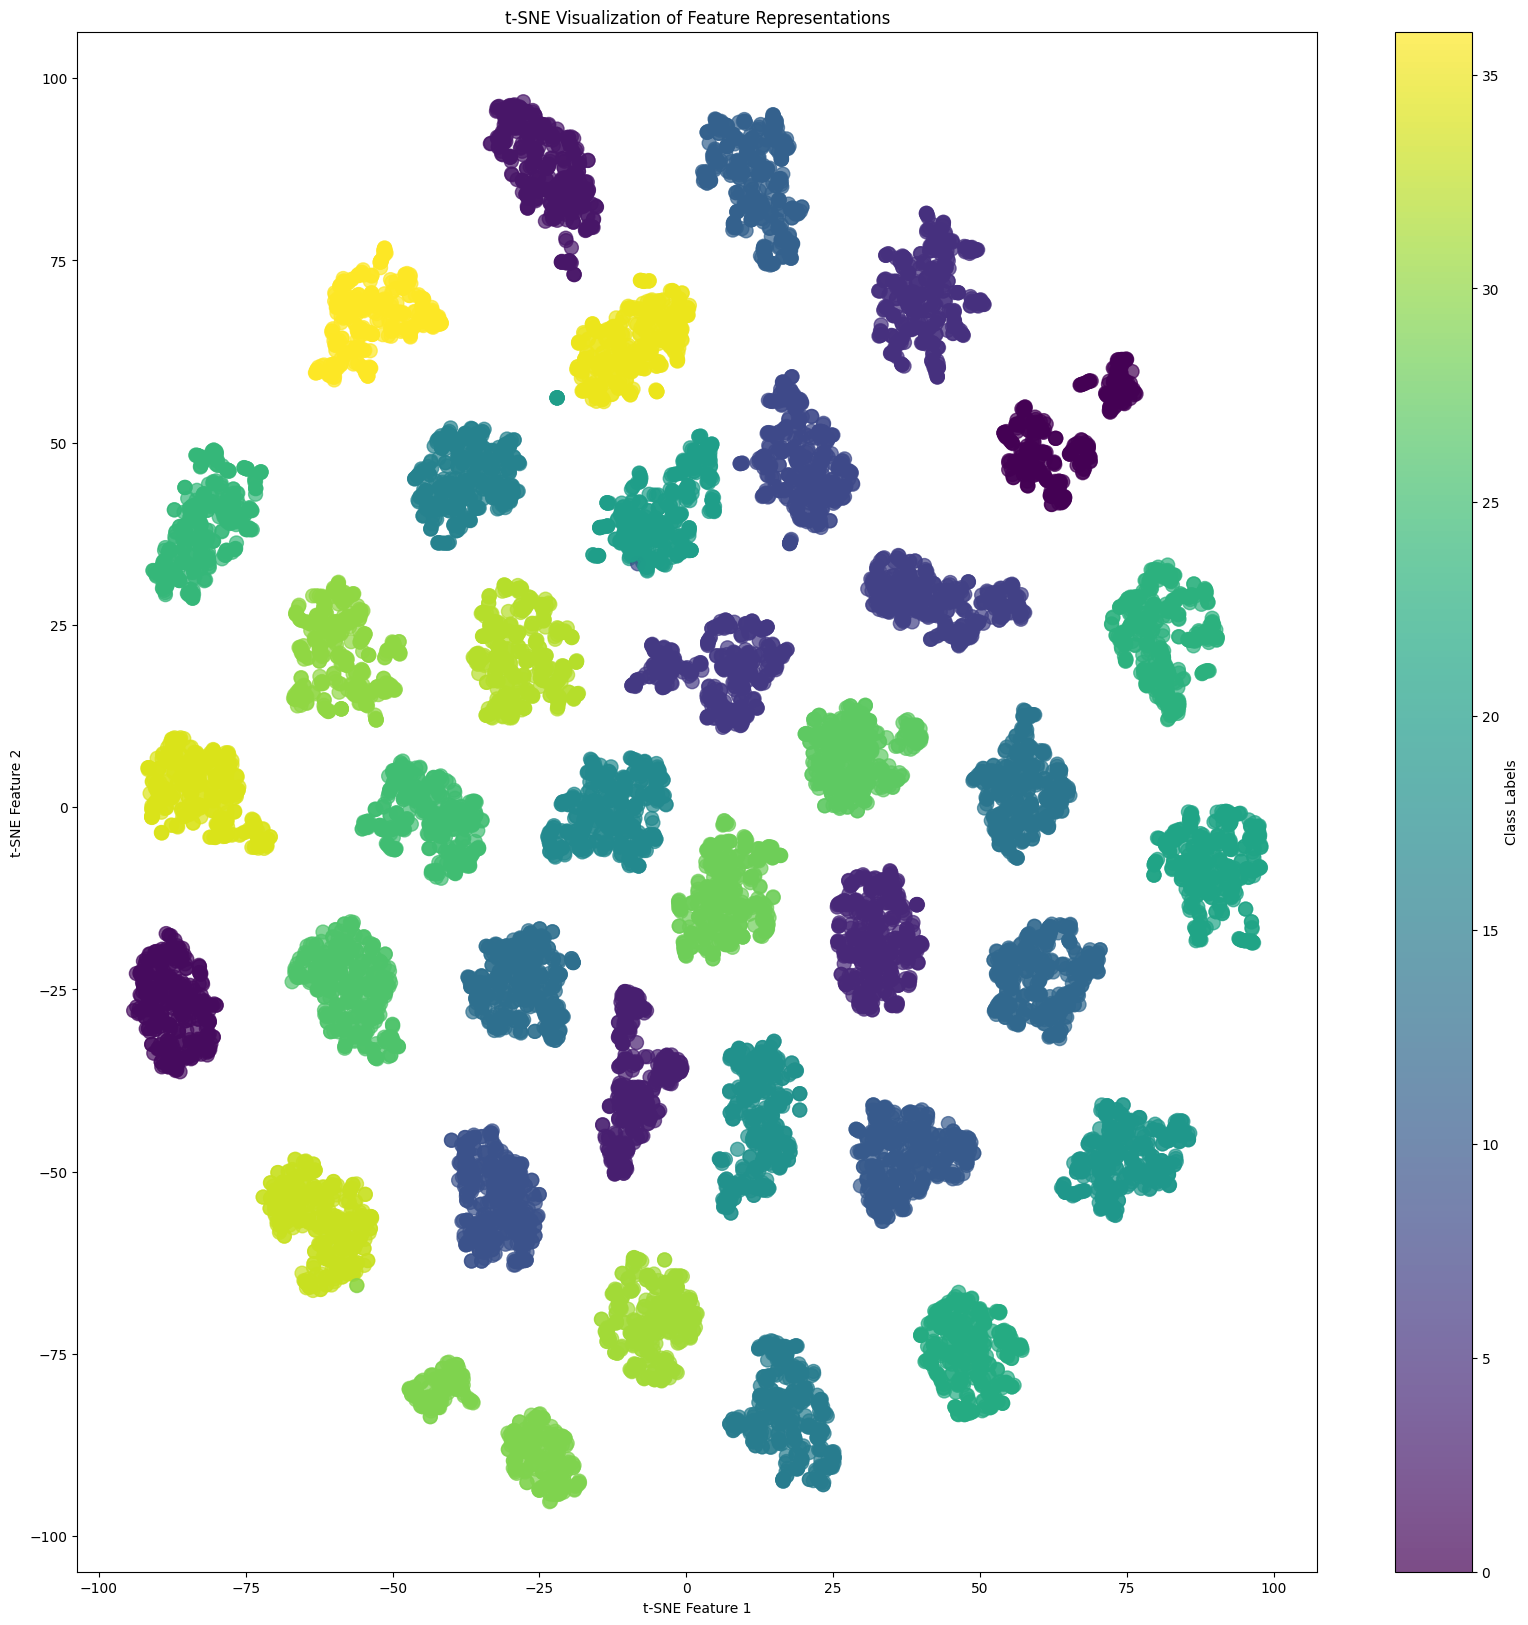
\includegraphics[width=0.41\textwidth]{Assets/tSNE/CONVNEXTBASE.png}
\captionof{figure}{CONVNEXTBASE}

\vspace{0.5cm}

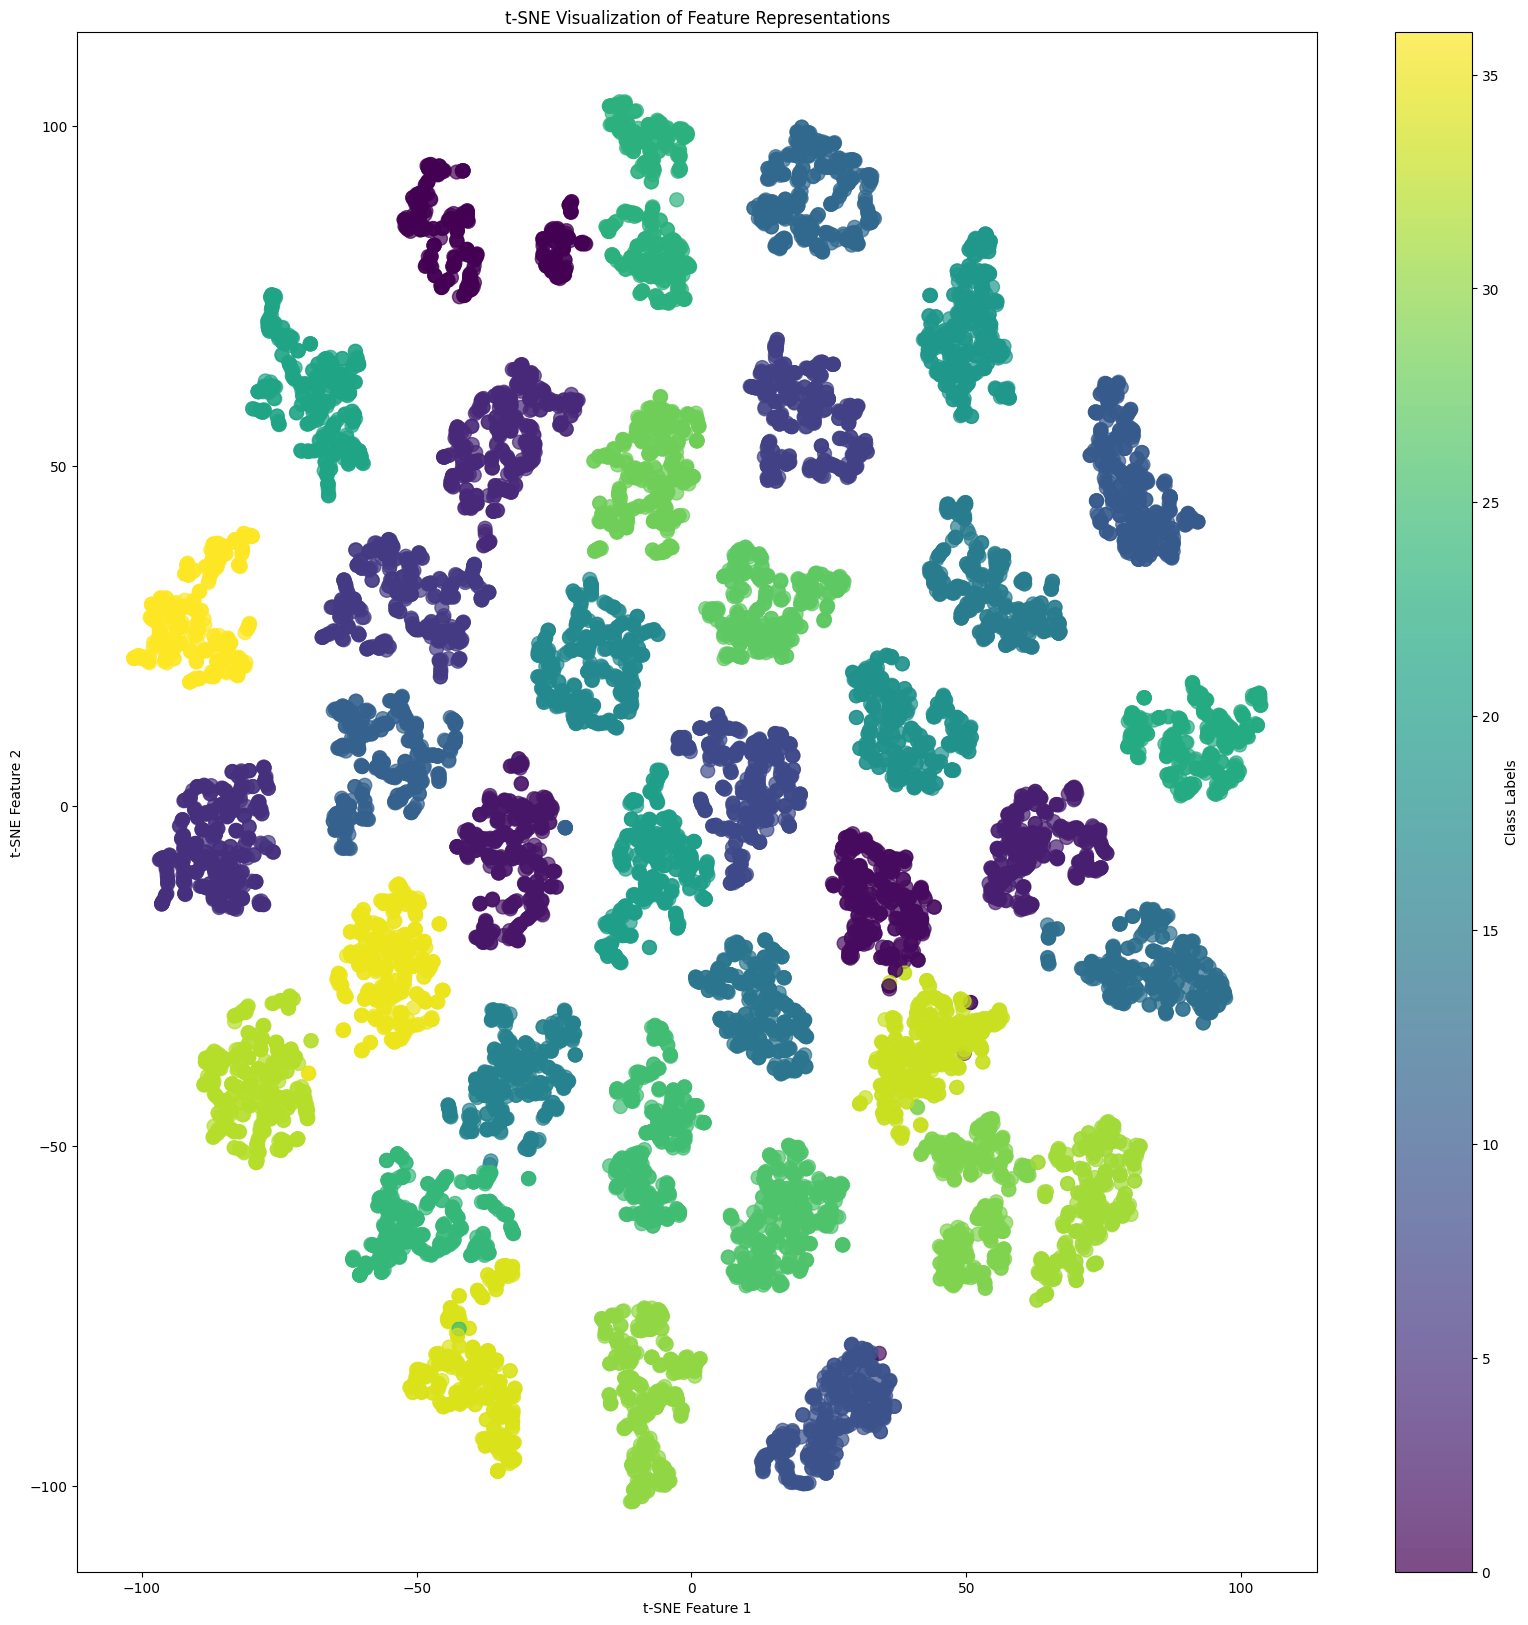
\includegraphics[width=0.41\textwidth]{Assets/tSNE/DenseNET121.png}
\captionof{figure}{DENSENET121}

\vspace{0.5cm}

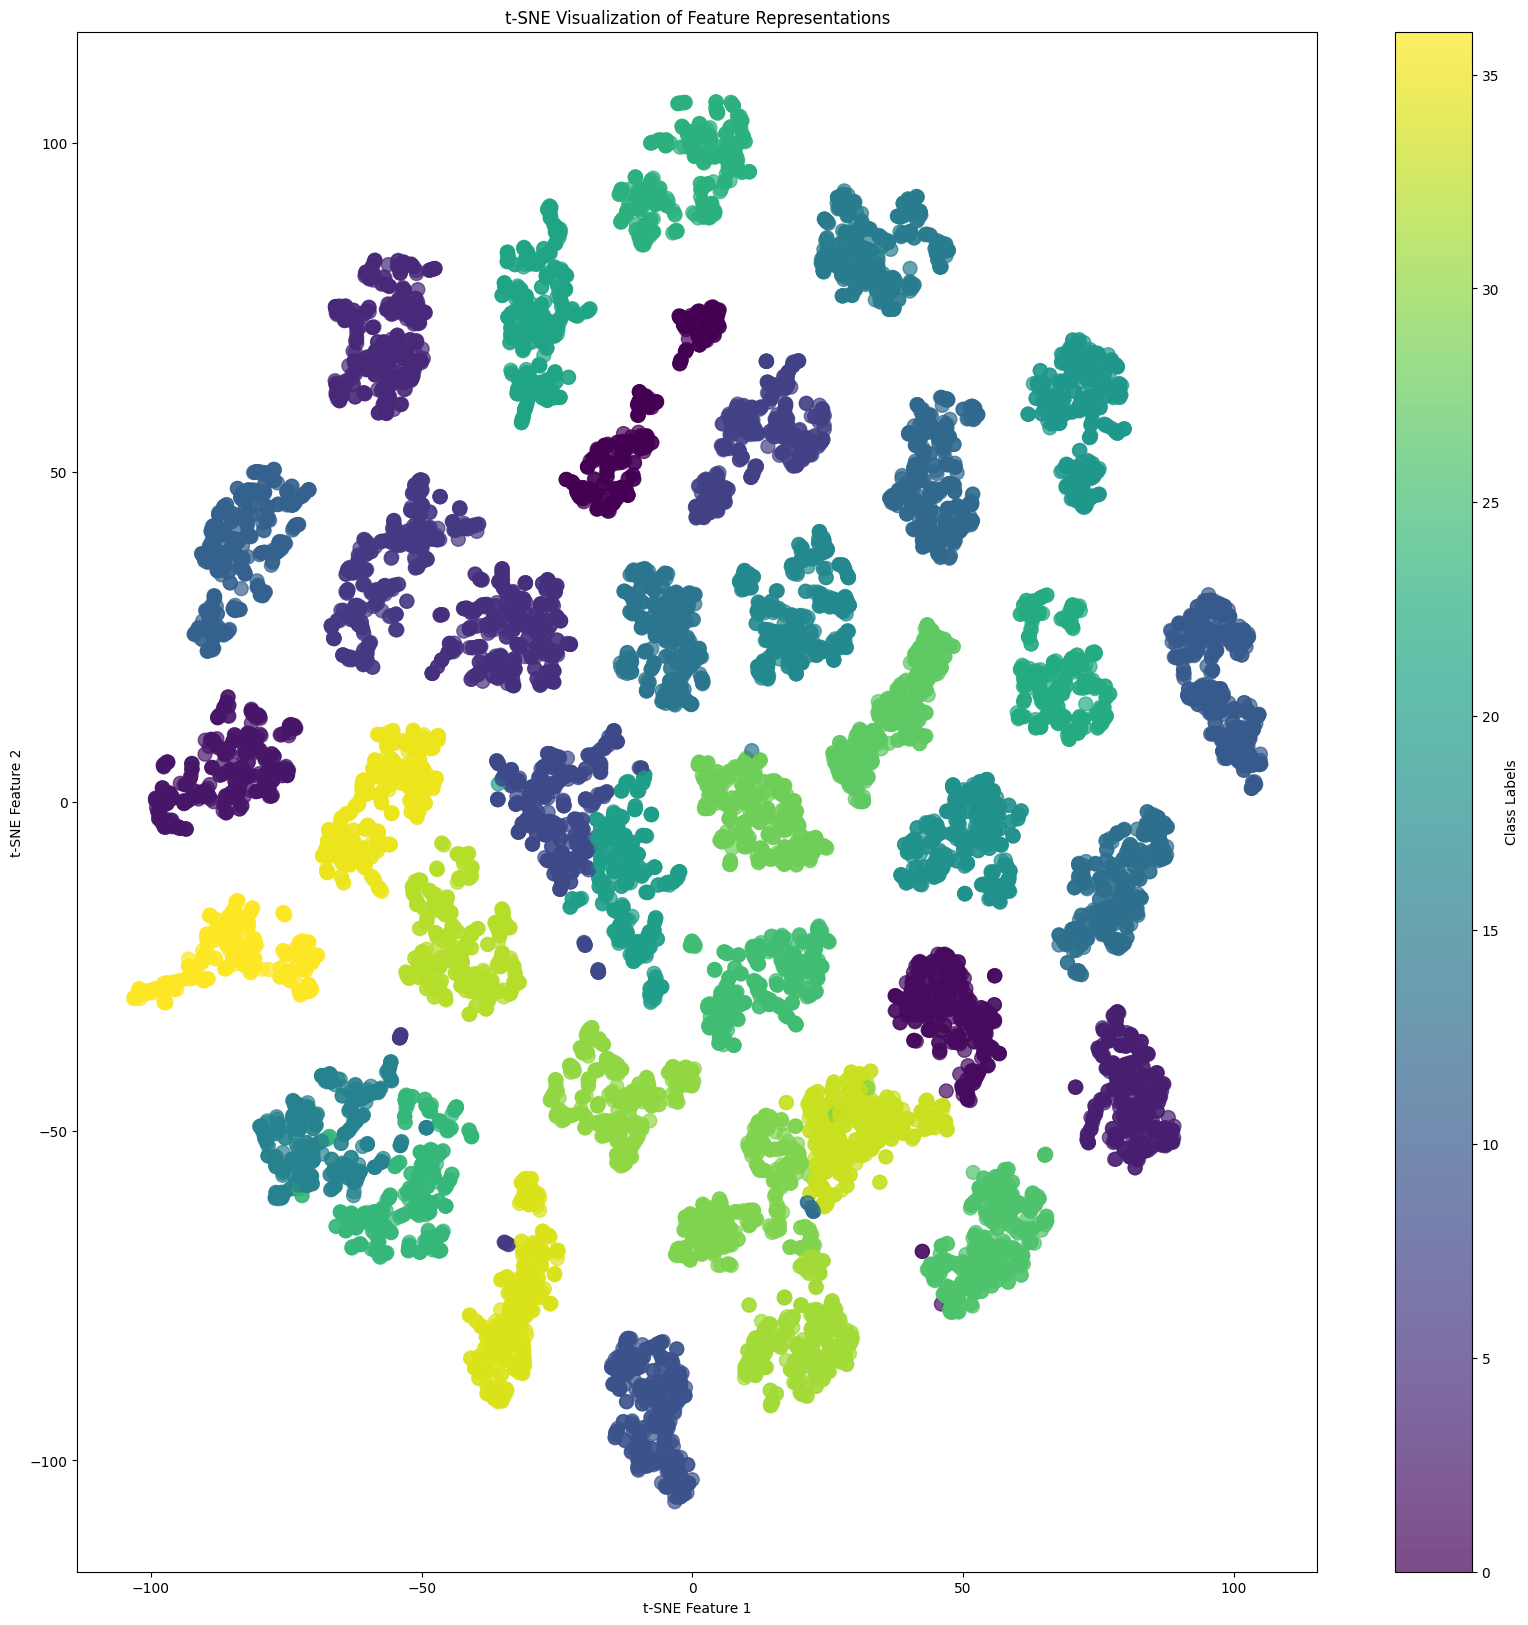
\includegraphics[width=0.41\textwidth]{Assets/tSNE/DenseNet169.png}
\captionof{figure}{DenseNet169}

\vspace{0.5cm}

\newpage

\includegraphics[width=0.45\textwidth]{Assets/tSNE/DENSENET201.png}
\captionof{figure}{DENSENET201}

\vspace{0.5cm}

\includegraphics[width=0.45\textwidth]{Assets/tSNE/EfficientNetB0.png}
\captionof{figure}{EfficientNetB0}

\vspace{0.5cm}


\includegraphics[width=0.45\textwidth]{Assets/tSNE/EfficientNetB0.png}
\captionof{figure}{EfficientNetB1}

\vspace{0.8cm}

\includegraphics[width=0.45\textwidth]{Assets/tSNE/EfficientNetV2L.png}
\captionof{figure}{EfficientNetV2L}

\vspace{0.8cm}

\newpage

\includegraphics[width=0.45\textwidth]{Assets/tSNE/MOBILENETV2.png}
\captionof{figure}{MOBILENETV2}

\vspace{0.8cm}

\includegraphics[width=0.45\textwidth]{Assets/tSNE/MobileNetV3Large.png}
\captionof{figure}{MobileNetV3Large}

\vspace{0.8cm}

\includegraphics[width=0.45\textwidth]{Assets/tSNE/ResNet50.png}
\captionof{figure}{ResNet50}

\vspace{0.8cm}

\includegraphics[width=0.45\textwidth]{Assets/tSNE/RESNET101.png}
\captionof{figure}{RESNET101}

\vspace{0.8cm}

\newpage

\includegraphics[width=0.45\textwidth]{Assets/tSNE/RESNET152.png}
\captionof{figure}{RESNET152}

\vspace{0.8cm}

\includegraphics[width=0.45\textwidth]{Assets/tSNE/vgg16.png}
\captionof{figure}{VGG16}

\vspace{0.8cm}

\end{multicols}


\renewcommand{\thefigure}{2.\arabic{figure}} % Prefix figures with "2."

\begin{center}
    \includegraphics[width=0.6\textwidth]{Assets/tSNE/CONVNEXT.png}
    \captionof{figure}{CONVNEXT}
\end{center}



\chapter*{Appendix-V: Gradcam HeatMaps}
\addcontentsline{toc}{chapter}{Appendix-V: Gradcam HeatMaps}

\noindent This appendix contains the Gradcam HeatMaps for all models.

\begin{multicols}{2}
\centering

\setcounter{figure}{0} % Reset figure counter
\renewcommand{\thefigure}{2.\arabic{figure}} % Prefix figures with "2."

\includegraphics[width=0.41\textwidth]{Assets/gradcam_heatmap/vgg19.png}
\captionof{figure}{VGG19}

\vspace{0.5cm}

\includegraphics[width=0.41\textwidth]{Assets/gradcam_heatmap/CONVNEXTBASE.png}
\captionof{figure}{CONVNEXTBASE}

\vspace{0.5cm}

\includegraphics[width=0.41\textwidth]{Assets/gradcam_heatmap/DenseNET121.png}
\captionof{figure}{DENSENET121}

\vspace{0.5cm}

\includegraphics[width=0.41\textwidth]{Assets/gradcam_heatmap/DenseNet169.png}
\captionof{figure}{DenseNet169}

\vspace{0.5cm}

\newpage

\includegraphics[width=0.45\textwidth]{Assets/gradcam_heatmap/DENSENET201.png}
\captionof{figure}{DENSENET201}

\vspace{0.8cm}

\includegraphics[width=0.45\textwidth]{Assets/gradcam_heatmap/EfficientNetB0.png}
\captionof{figure}{EfficientNetB0}

\vspace{0.8cm}


\includegraphics[width=0.45\textwidth]{Assets/gradcam_heatmap/EfficientNetB0.png}
\captionof{figure}{EfficientNetB1}

\vspace{0.8cm}

\includegraphics[width=0.45\textwidth]{Assets/gradcam_heatmap/EfficientNetV2L.png}
\captionof{figure}{EfficientNetV2L}

\vspace{0.8cm}

\newpage

\includegraphics[width=0.45\textwidth]{Assets/gradcam_heatmap/MOBILENETV2.png}
\captionof{figure}{MOBILENETV2}

\vspace{0.8cm}

\includegraphics[width=0.45\textwidth]{Assets/gradcam_heatmap/MobileNetV3Large.png}
\captionof{figure}{MobileNetV3Large}

\vspace{0.8cm}

\includegraphics[width=0.45\textwidth]{Assets/gradcam_heatmap/ResNet50.png}
\captionof{figure}{ResNet50}

\vspace{0.8cm}

\includegraphics[width=0.45\textwidth]{Assets/gradcam_heatmap/RESNET101.png}
\captionof{figure}{RESNET101}

\vspace{0.8cm}

\newpage

\includegraphics[width=0.45\textwidth]{Assets/gradcam_heatmap/RESNET152.png}
\captionof{figure}{RESNET152}

\vspace{0.8cm}

\includegraphics[width=0.45\textwidth]{Assets/gradcam_heatmap/vgg16.png}
\captionof{figure}{VGG16}

\vspace{0.8cm}

\end{multicols}


\renewcommand{\thefigure}{2.\arabic{figure}} % Prefix figures with "2."

\begin{center}
    \includegraphics[width=0.6\textwidth]{Assets/gradcam_heatmap/CONVNEXT.png}
    \captionof{figure}{CONVNEXT}
\end{center}



\chapter*{Appendix-VI: Lime Visualizations}
\addcontentsline{toc}{chapter}{Appendix-VI: Lime Visualizations}

\noindent This appendix contains the Lime Visualizations for all models.

\begin{multicols}{2}
\centering

\setcounter{figure}{0} % Reset figure counter
\renewcommand{\thefigure}{2.\arabic{figure}} % Prefix figures with "2."

\includegraphics[width=0.41\textwidth]{Assets/lime_visualization/vgg19.png}
\captionof{figure}{VGG19}

\vspace{0.5cm}

\includegraphics[width=0.41\textwidth]{Assets/lime_visualization/CONVNEXTBASE.png}
\captionof{figure}{CONVNEXTBASE}

\vspace{0.5cm}

\includegraphics[width=0.41\textwidth]{Assets/lime_visualization/DenseNET121.png}
\captionof{figure}{DENSENET121}

\vspace{0.5cm}

\includegraphics[width=0.41\textwidth]{Assets/lime_visualization/DenseNet169.png}
\captionof{figure}{DenseNet169}

\vspace{0.5cm}

\newpage

\includegraphics[width=0.45\textwidth]{Assets/lime_visualization/DENSENET201.png}
\captionof{figure}{DENSENET201}

\vspace{0.8cm}

\includegraphics[width=0.45\textwidth]{Assets/lime_visualization/EfficientNetB0.png}
\captionof{figure}{EfficientNetB0}

\vspace{0.8cm}


\includegraphics[width=0.45\textwidth]{Assets/lime_visualization/EfficientNetB0.png}
\captionof{figure}{EfficientNetB1}

\vspace{0.8cm}

\includegraphics[width=0.45\textwidth]{Assets/lime_visualization/EfficientNetV2L.png}
\captionof{figure}{EfficientNetV2L}

\vspace{0.8cm}

\newpage

\includegraphics[width=0.45\textwidth]{Assets/lime_visualization/MOBILENETV2.png}
\captionof{figure}{MOBILENETV2}

\vspace{0.8cm}

\includegraphics[width=0.45\textwidth]{Assets/lime_visualization/MobileNetV3Large.png}
\captionof{figure}{MobileNetV3Large}

\vspace{0.8cm}

\includegraphics[width=0.45\textwidth]{Assets/lime_visualization/ResNet50.png}
\captionof{figure}{ResNet50}

\vspace{0.8cm}

\includegraphics[width=0.45\textwidth]{Assets/lime_visualization/RESNET101.png}
\captionof{figure}{RESNET101}

\vspace{0.8cm}

\newpage

\includegraphics[width=0.45\textwidth]{Assets/lime_visualization/RESNET152.png}
\captionof{figure}{RESNET152}

\vspace{0.8cm}

\includegraphics[width=0.45\textwidth]{Assets/lime_visualization/vgg16.png}
\captionof{figure}{VGG16}

\vspace{0.8cm}

\end{multicols}


\renewcommand{\thefigure}{2.\arabic{figure}} % Prefix figures with "2."

\begin{center}
    \includegraphics[width=0.6\textwidth]{Assets/lime_visualization/CONVNEXT.png}
    \captionof{figure}{CONVNEXT}
\end{center}




% Ref
\bibliographystyle{plain}
\bibliography{ref}

\end{document}


